%% (Master) Thesis template
% Template version used: v1.4
%
% Largely adapted from Adrian Nievergelt's template for the ADPS
% (lecture notes) project.


%% We use the memoir class because it offers a many easy to use features.
\documentclass[11pt,a4paper,titlepage]{memoir}

%% Packages
%% ========

%% LaTeX Font encoding -- DO NOT CHANGE
\usepackage[OT1]{fontenc}

%% Babel provides support for languages.  'english' uses British
%% English hyphenation and text snippets like "Figure" and
%% "Theorem". Use the option 'ngerman' if your document is in German.
%% Use 'american' for American English.  Note that if you change this,
%% the next LaTeX run may show spurious errors.  Simply run it again.
%% If they persist, remove the .aux file and try again.
\usepackage[english]{babel}

%% Input encoding 'utf8'. In some cases you might need 'utf8x' for
%% extra symbols. Not all editors, especially on Windows, are UTF-8
%% capable, so you may want to use 'latin1' instead.
\usepackage[utf8]{inputenc}

%% This changes default fonts for both text and math mode to use Herman Zapfs
%% excellent Palatino font.  Do not change this.
\usepackage[sc]{mathpazo}

%% The AMS-LaTeX extensions for mathematical typesetting.  Do not
%% remove.
\usepackage{amsmath,amssymb,amsfonts,mathrsfs}

%% NTheorem is a reimplementation of the AMS Theorem package. This
%% will allow us to typeset theorems like examples, proofs and
%% similar.  Do not remove.
%% NOTE: Must be loaded AFTER amsmath, or the \qed placement will
%% break
\usepackage[amsmath,thmmarks]{ntheorem}

%% LaTeX' own graphics handling
\usepackage{graphicx}

%% We unfortunately need this for the Rules chapter.  Remove it
%% afterwards; or at least NEVER use its underlining features.
\usepackage{soul}

%% This allows you to add .pdf files. It is used to add the
%% declaration of originality.
\usepackage{pdfpages}

%% Some more packages that you may want to use.  Have a look at the
%% file, and consult the package docs for each.
%% See the TeXed file for more explanations
%% [REC] Format dates and time depending on locale
\usepackage{datetime}

%% [OPT] Multi-rowed cells in tabulars
%\usepackage{multirow}

%% [REC] Intelligent cross reference package. This allows for nice
%% combined references that include the reference and a hint to where
%% to look for it.

\usepackage{varioref}

%% [OPT] Easily changeable quotes with \enquote{Text}
%\usepackage[german=swiss]{csquotes}



%% [OPT] Provides a \cancel{} command to stroke through mathematics.
%\usepackage{cancel}

%% [NEED] This allows for additional typesetting tools in mathmode.
%% See its excellent documentation.
\usepackage{mathtools}

%% [ADV] Conditional commands
%\usepackage{ifthen}

%% [OPT] Manual large braces or other delimiters.
%\usepackage{bigdelim, bigstrut}

%% [REC] Alternate vector arrows. Use the command \vv{} to get scaled
%% vector arrows.
\usepackage[h]{esvect}

%% [NEED] Some extensions to tabulars and array environments.
\usepackage{array}

%% [OPT] Postscript support via pstricks graphics package. Very
%% diverse applications.
%\usepackage{pstricks,pst-all}

%% [?] This seems to allow us to define some additional counters.
%\usepackage{etex}

%% [ADV] XY-Pic to typeset some matrix-style graphics
%\usepackage[all]{xy}

%% [OPT] This is needed to generate an index at the end of the
%% document.
%\usepackage{makeidx}

%% [OPT] Fancy package for source code listings.  The template text
%% needs it for some LaTeX snippets; remove/adapt the \lstset when you
%% remove the template content.
\usepackage{listings}
\lstset{language=TeX,basicstyle={\normalfont\ttfamily}}

%% [REC] Fancy character protrusion.  Must be loaded after all fonts.
\usepackage[activate]{pdfcprot}

%% [REC] Nicer tables.  Read the excellent documentation.
\usepackage{booktabs}

%% lmodern removes this restriction by allowing font sizes at arbitrary sizes
\usepackage{lmodern}


%% Our layout configuration.  DO NOT CHANGE.
%% Memoir layout setup

%% NOTE: You are strongly advised not to change any of them unless you
%% know what you are doing.  These settings strongly interact in the
%% final look of the document.

% Dependencies
\usepackage{UNIGElogo}

% Turn extra space before chapter headings off.
\setlength{\beforechapskip}{0pt}

\nonzeroparskip
\parindent=0pt
\defaultlists

% Chapter style redefinition
\makeatletter

\if@twoside
  \pagestyle{Ruled}
  \copypagestyle{chapter}{Ruled}
\else
  \pagestyle{ruled}
  \copypagestyle{chapter}{ruled}
\fi
\makeoddhead{chapter}{}{}{}
\makeevenhead{chapter}{}{}{}
\makeheadrule{chapter}{\textwidth}{0pt}
\copypagestyle{abstract}{empty}

\makechapterstyle{bianchimod}{%
  \chapterstyle{default}
  \renewcommand*{\chapnamefont}{\normalfont\Large\sffamily}
  \renewcommand*{\chapnumfont}{\normalfont\Large\sffamily}
  \renewcommand*{\printchaptername}{%
    \chapnamefont\centering\@chapapp}
  \renewcommand*{\printchapternum}{\chapnumfont {\thechapter}}
  \renewcommand*{\chaptitlefont}{\normalfont\huge\sffamily}
  \renewcommand*{\printchaptertitle}[1]{%
    \hrule\vskip\onelineskip \centering \chaptitlefont\textbf{\vphantom{gyM}##1}\par}
  \renewcommand*{\afterchaptertitle}{\vskip\onelineskip \hrule\vskip
    \afterchapskip}
  \renewcommand*{\printchapternonum}{%
    \vphantom{\chapnumfont {9}}\afterchapternum}}

% Use the newly defined style
\chapterstyle{bianchimod}

\setsecheadstyle{\Large\bfseries\sffamily}
\setsubsecheadstyle{\large\bfseries\sffamily}
\setsubsubsecheadstyle{\bfseries\sffamily}
\setparaheadstyle{\normalsize\bfseries\sffamily}
\setsubparaheadstyle{\normalsize\itshape\sffamily}
\setsubparaindent{0pt}

% Set captions to a more separated style for clearness
\captionnamefont{\sffamily\bfseries\footnotesize}
\captiontitlefont{\sffamily\footnotesize}
\setlength{\intextsep}{16pt}
\setlength{\belowcaptionskip}{1pt}

% Set section and TOC numbering depth to subsection
\setsecnumdepth{subsection}
\settocdepth{subsection}

%% Titlepage adjustments
\pretitle{\vspace{10pt plus 0.7fill}\begin{center}\HUGE\sffamily\bfseries}
\posttitle{\end{center}\par}
\preauthor{\par\begin{center}\let\and\\\Large\sffamily}
\postauthor{\end{center}}
\predate{\par\begin{center}\Large\sffamily}
\postdate{\end{center}}

\def\@advisors{}
\newcommand{\advisors}[1]{\def\@advisors{#1}}
\def\@department{}
\newcommand{\department}[1]{\def\@department{#1}}
\def\@thesistype{}
\newcommand{\thesistype}[1]{\def\@thesistype{#1}}

\renewcommand{\maketitlehooka}{\noindent\UNIGElogo[3in]}

\renewcommand{\maketitlehookb}{\vspace{1in}%
  \par\begin{center}\Large\sffamily\@thesistype\end{center}}

\renewcommand{\maketitlehookd}{%
  \vfill\par
  \begin{flushright}
    \sffamily
    \@advisors\par
    \@department, UNIGE Geneva
  \end{flushright}
}

\checkandfixthelayout

\setlength{\droptitle}{-48pt}

\makeatother

% This defines how theorems should look. Best leave as is.
\theoremstyle{plain}
\setlength\theorempostskipamount{0pt}

%%% Local Variables:
%%% mode: latex
%%% TeX-master: "thesis"
%%% End:


%% Theorem environments.  You will have to adapt this for a German
%% thesis.
%% Theorem-like environments

%% This can be changed according to language. You can comment out the ones you
%% don't need.

\numberwithin{equation}{chapter}

%% German theorems
%\newtheorem{satz}{Satz}[chapter]
%\newtheorem{beispiel}[satz]{Beispiel}
%\newtheorem{bemerkung}[satz]{Bemerkung}
%\newtheorem{korrolar}[satz]{Korrolar}
%\newtheorem{definition}[satz]{Definition}
%\newtheorem{lemma}[satz]{Lemma}
%\newtheorem{proposition}[satz]{Proposition}

%% English variants
\newtheorem{theorem}{Theorem}[chapter]
\newtheorem{example}[theorem]{Example}
\newtheorem{remark}[theorem]{Remark}
\newtheorem{corollary}[theorem]{Corollary}
\newtheorem{definition}[theorem]{Definition}
\newtheorem{lemma}[theorem]{Lemma}
\newtheorem{proposition}[theorem]{Proposition}

%% Proof environment with a small square as a "qed" symbol
\theoremstyle{nonumberplain}
\theorembodyfont{\normalfont}
\theoremsymbol{\ensuremath{\square}}
\newtheorem{proof}{Proof}
%\newtheorem{beweis}{Beweis}


%% Helpful macros.
%% Custom commands
%% ===============

%% Special characters for number sets, e.g. real or complex numbers.
\newcommand{\C}{\mathbb{C}}
\newcommand{\K}{\mathbb{K}}
\newcommand{\N}{\mathbb{N}}
\newcommand{\Q}{\mathbb{Q}}
\newcommand{\R}{\mathbb{R}}
\newcommand{\Z}{\mathbb{Z}}
\newcommand{\X}{\mathbb{X}}

%% Fixed/scaling delimiter examples (see mathtools documentation)
\DeclarePairedDelimiter\abs{\lvert}{\rvert}
\DeclarePairedDelimiter\norm{\lVert}{\rVert}

%% Use the alternative epsilon per default and define the old one as \oldepsilon
\let\oldepsilon\epsilon
\renewcommand{\epsilon}{\ensuremath\varepsilon}

%% Also set the alternate phi as default.
\let\oldphi\phi
\renewcommand{\phi}{\ensuremath{\varphi}}


%% Make document internal hyperlinks wherever possible. (TOC, references)
%% This MUST be loaded after varioref, which is loaded in 'extrapackages'
%% above.  We just load it last to be safe.
\usepackage[linkcolor=black,colorlinks=true,citecolor=black,filecolor=black]{hyperref}

%% colour manipulation
\usepackage{color}
\usepackage{float}

%% comment on marjin
\usepackage{mparhack}
\usepackage[colorinlistoftodos]{todonotes}%% go to todofeaturepage to see the feature of todo package
\usepackage{marginnote}
\usepackage[top=1.5cm, bottom=1.5cm, outer=5cm, inner=2cm, heightrounded, marginparwidth=2.5cm, marginparsep=2cm]{geometry}


%% Document information
%% ====================

\title{Comparing Digital Platforms for Challenge-based Learning}
\author{M. O. Darwich}
\thesistype{Master Thesis}
\advisors{Advisors: Prof. Fran\c{c}ois Grey }
\department{Department of Computer Science}
\date{\today}

\begin{document}

\frontmatter

%% Title page is autogenerated from document information above.  DO
%% NOT CHANGE.
\begin{titlingpage}
  \calccentering{\unitlength}
  \begin{adjustwidth*}{\unitlength-24pt}{-\unitlength-24pt}
    \maketitle
  \end{adjustwidth*}
\end{titlingpage}

%% The abstract of your thesis.  Edit the file as needed.
\begin{abstract}
  This example thesis briefly shows the main features of our thesis
  style, and how to use it for your purposes.
\end{abstract}


%% TOC with the proper setup, do not change.
\cleartorecto
\tableofcontents
\mainmatter
\listoftodos
%% Your real content!
% Some commands used in this file
\newcommand{\package}{\emph}

\chapter{Introduction}



\chapter{History of platform with 2 case study}

\section{History of documentation platforms}

In the maker - movement \cite{davies2017hackerspaces}, people need online tools to exchange knowledge, share experiences and to work in interdisciplinary teams to \textit{innovate}, \textit{design} and \textit{implement solutions}.

The method of online documentation has a strong influence on how useful, learnable, available, shareable and accessible results are \cite{harcourt2016re}.

\todo{add my story}
The complexity of documentation has led makers to create a variety of online communities and to experiment with different ways of documenting their results. Because documentation is often seen as tedious and time-consuming, makers are constantly seeking optimal solutions to reduce the effort needed to document their results. On the other hand, careful documentation enables makers to collaborate and share their efforts more effectively.


In the following, we will briefly survey a range of platforms developed to support makers in documenting their projects. We then analyze in more detail the pros and cons of two platforms, \textit{Instructables} and \textit{Build-in-Progress}. In both case we discuss how authors and readers benefit from online documentation, what motivates them to share a project and – in the case of \textit{Build-in-Progress} what are the consequences of sharing a work in progress with online community.

The first section will review \textit{Instructables}, describe how the platform works and describe in details the design orientation process. The second section will review the design approach of \textit{SDG-in-Progress} and the added features. The last part will review the user interaction of \textit{BiP}. 


\todo{History of platform}
\todo{Timline of different platform}
\todo{properties}s
Github, wiki, instructable etc..

\begin{itemize}
	\item Time line of different platform : when it started, stopped or still used
	\item Properties of platform
\end{itemize}

\section{Instructable}


\begin{center}
	\begin{minipage}{.7\textwidth}
		\textit{In this section, I share with you an analyses of how users create and share \textit{DIY} projects via online platform called Instructables. I share findings of the analyses of this platform and the understanding of how authors and users use Instructables}
	\end{minipage}
\end{center}

\begin{comment}
\hl{What is it ?} \hl{Who use it ?} \hl{User interactions ?} \hl{Limitations} \hl{Advantages ?} \hl{Examples ?} \\
\end{comment}

\begin{figure}[ht!]
	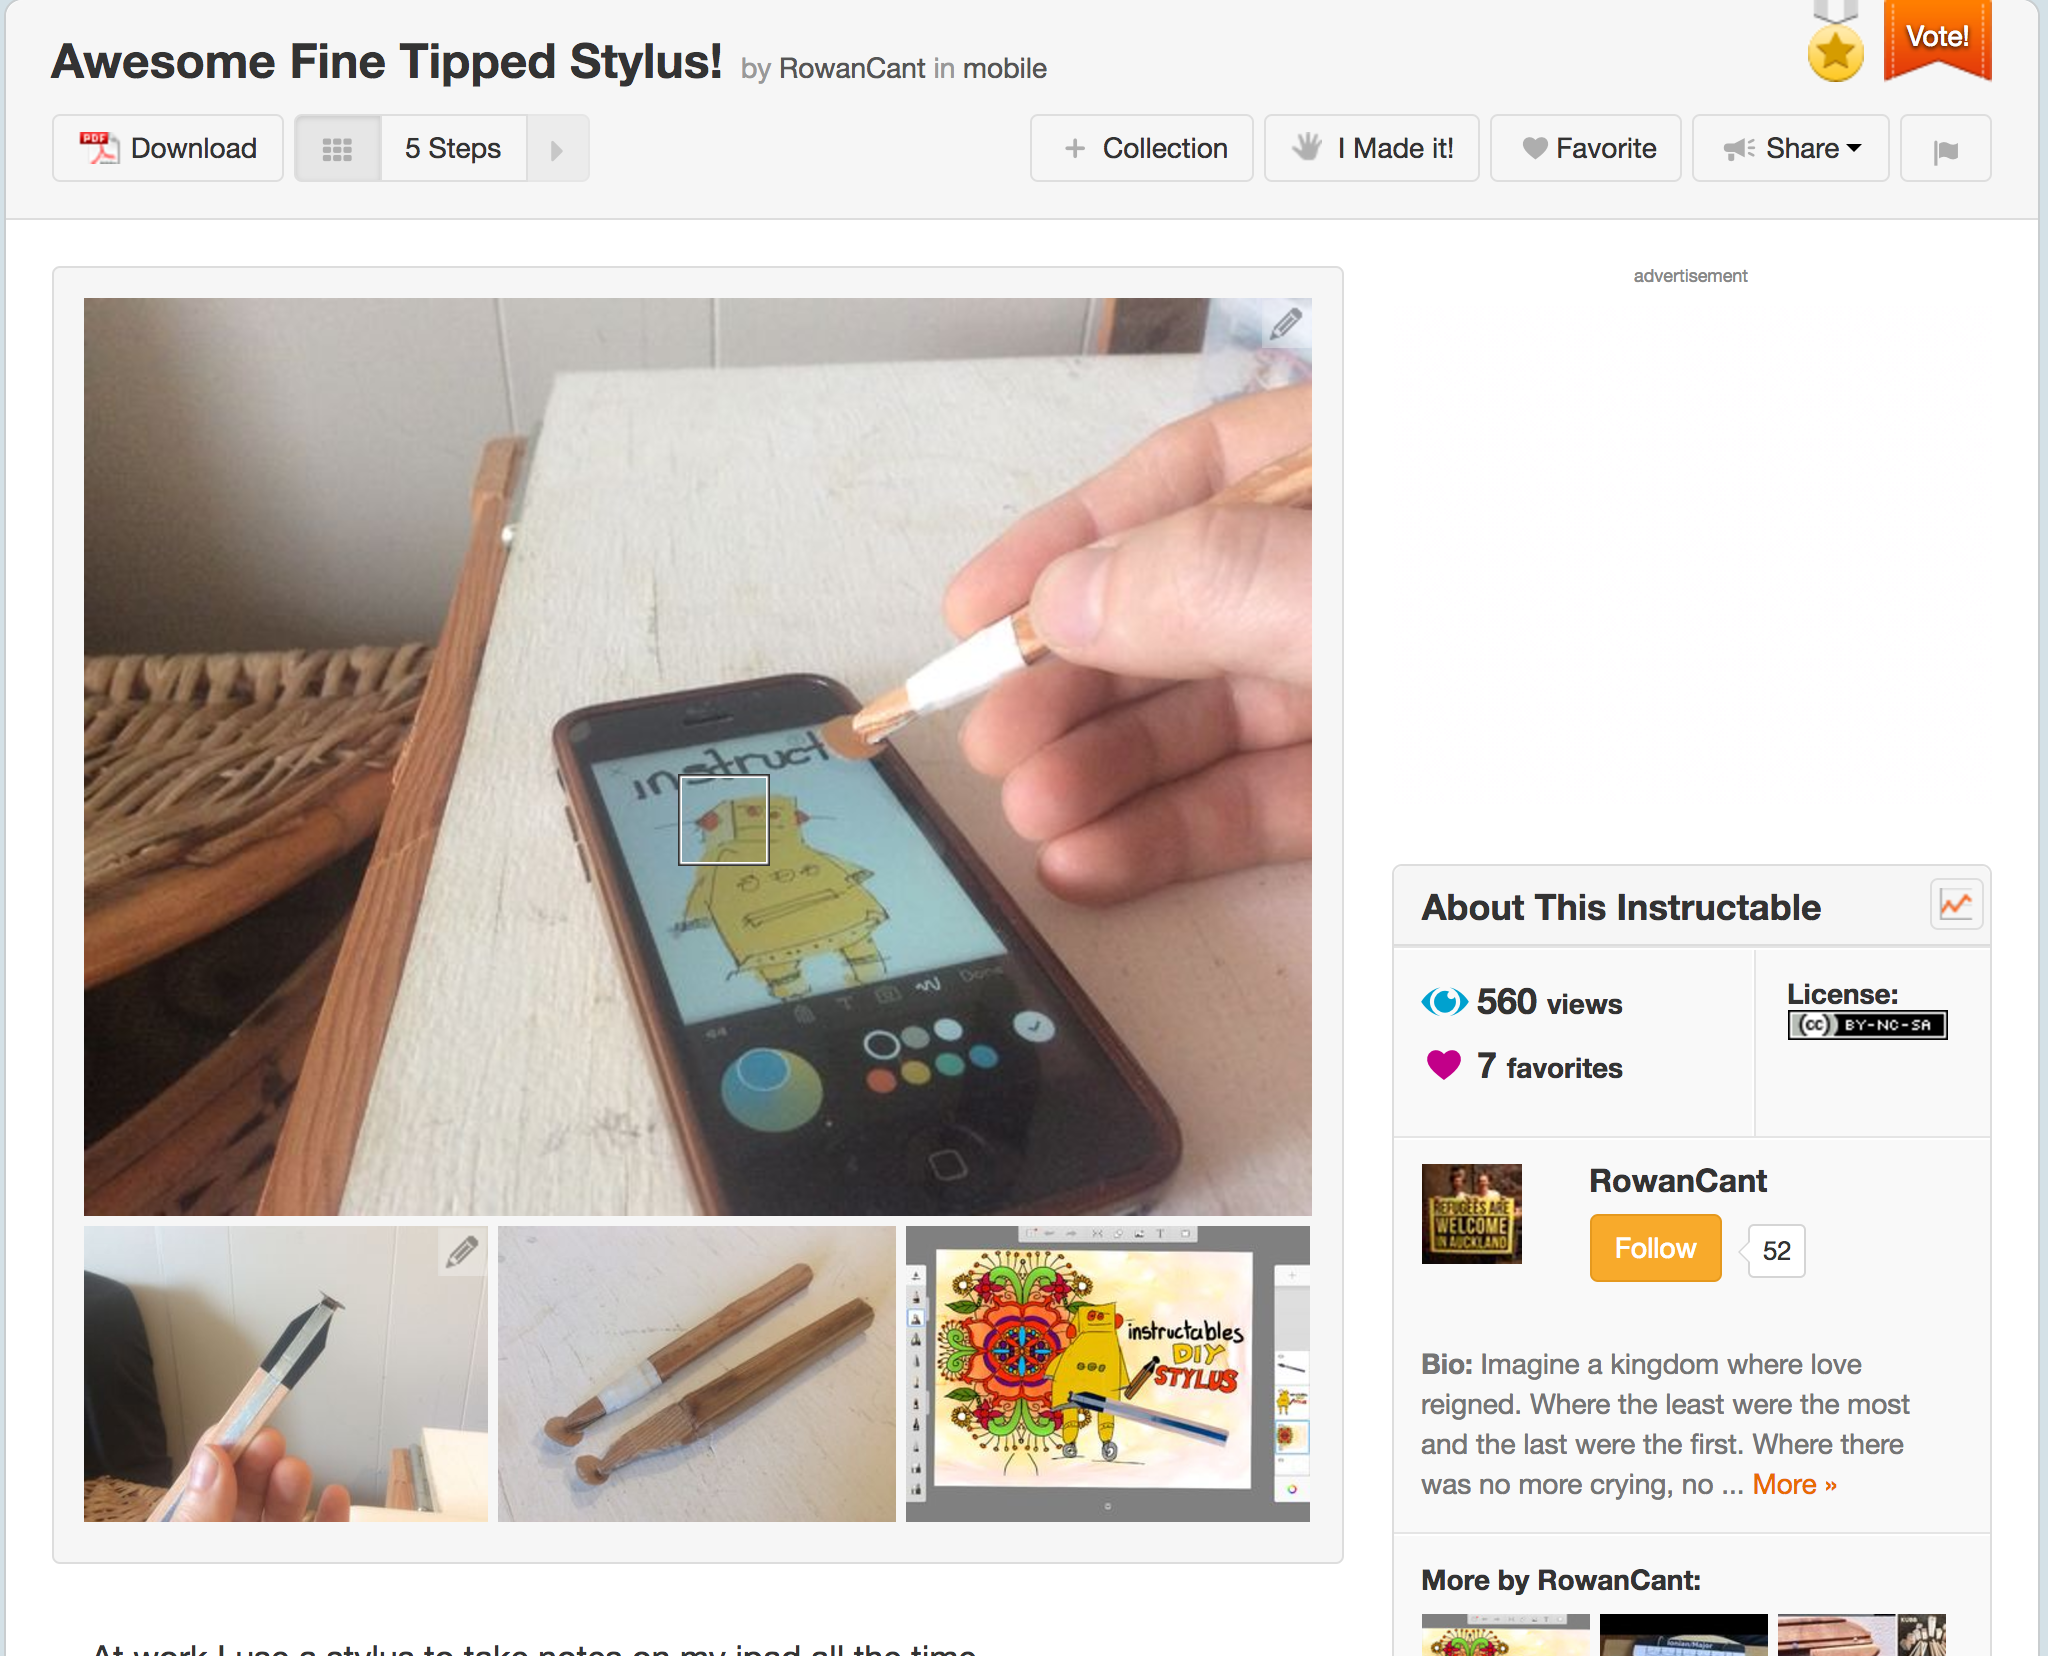
\includegraphics[scale=0.36]{./images/img-instructables.png}
	\caption{Sample Instructables project, \url{http://www.instructables.com/id/Awesome-Fine-Tipped-Stylus/}}
	\label{fig:sipillustration}
\end{figure}

Instructables is an online platform for \textit{DIY} communities that serves as a "place that lets you explore, document, and share your creations", it is a website specializing in user-created and uploaded do-it-yourself projects, which other users can comment on and rate for quality \cite{wiki:instructable}. There are different categories of project such as technology, crafts, food, home, workshops and living, with more than 263,258 projects and 9,888,442 monthly visit as of August 2017. Users create their project step by step and with each step they describe what they did in a text, photos or videos as displayed in the figure \ref{fig:sipillustration}.  Encapsulation of steps produce a typical guide that help others to re-create the project, learn from it or build a new thing on top of it and have their own version of the project. 

The contributions in Instructables come from the sharing culture of projects, not only authors contribute but also readers who can view and give feedback by commenting on the project. Also, Instructables create a social community where they exchange their thoughts about a topic via forums and sub-forums dedicated to a special topic such as Arduino projects. Finally, prizes are given to the top shared Instructables as a kind of reward for their effort of sharing their project and to keep them connected with the community.

\subsection{Methodology} 

To understand the users interactions of Instructables, an extensive study of the Instructables community has been done in the fall of 2011, this study used semi-structured interviews and online surveys. The semi-structured interviews had a framework of four themes that had been explored : (\oldstylenums{1}) motivation, (\oldstylenums{2}) Documentation tools, (\oldstylenums{3}) Writing an Instructable and (\oldstylenums{4}) Feedback. A theme was covered by a set of questions that took one hour with each interviewer. \cite{scholar:Tseng:2014:PVP:2598510.2598540}. A survey of 15 multiple-choice questions and open ended-questions that ask users about different aspects of their experience with replicating or building on top of a project shared by a user on the platform.

\subsection{User interaction}

The study has shown three strategies for documenting a project. The first was to \textit{write after you make}, as shown in the figure \ref{img-writemake}  \cite{tseng2016making}.
\begin{figure}[ht!]
	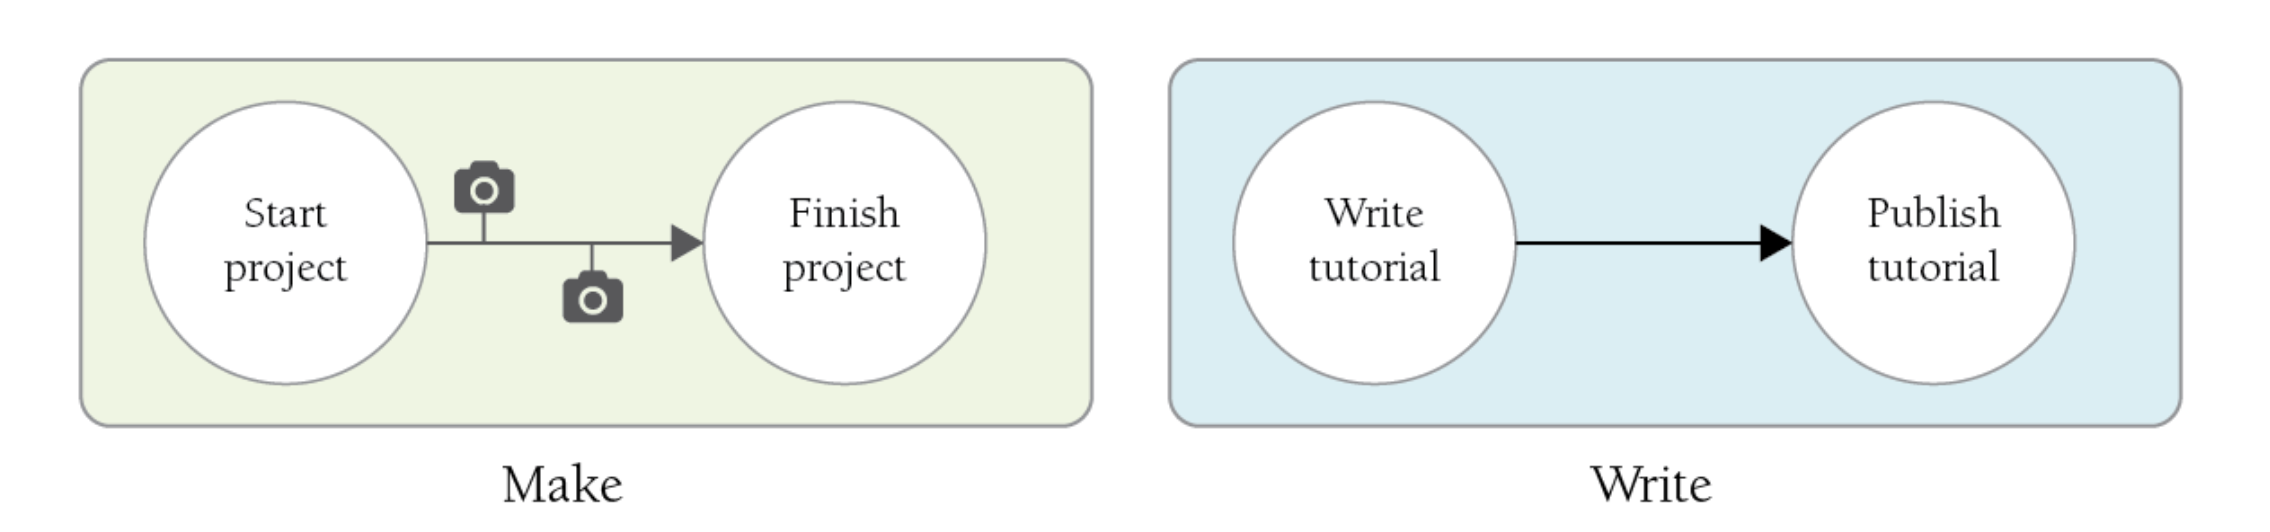
\includegraphics[scale=0.34]{./images/img-writemake.png}
	\caption{First strategy of documenting : write after you make, \cite{tseng2016making}}
	\label{img-writemake}
\end{figure}

A problem confronted the users with this strategy, users forgot to document in the midst of making. Users outperformed this problem by following the second strategy of \textit{writing after replicating}, as displayed in the figure \ref{img-makereplicatewrite} \cite{scholar:Tseng:2014:PVP:2598510.2598540}
\begin{figure}[ht!]
	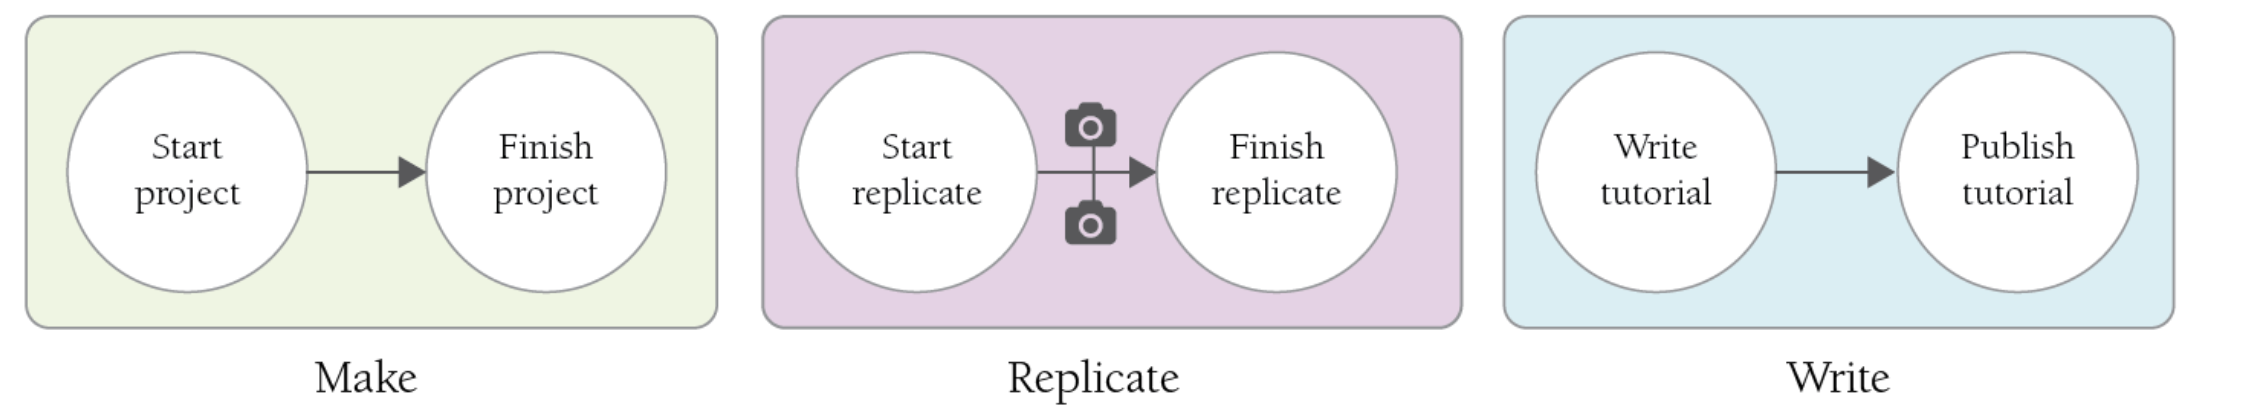
\includegraphics[scale=0.34]{./images/img-makereplicatewrite.png}
	\caption{First strategy of documenting : Make, replicate  then write, \cite{tseng2016making}}
	\label{img-makereplicatewrite}
\end{figure}

The final strategy was to \textit{simultaneously write and make} (figure \ref{img-makewritesimultanously}). 
\begin{figure}[ht!]
	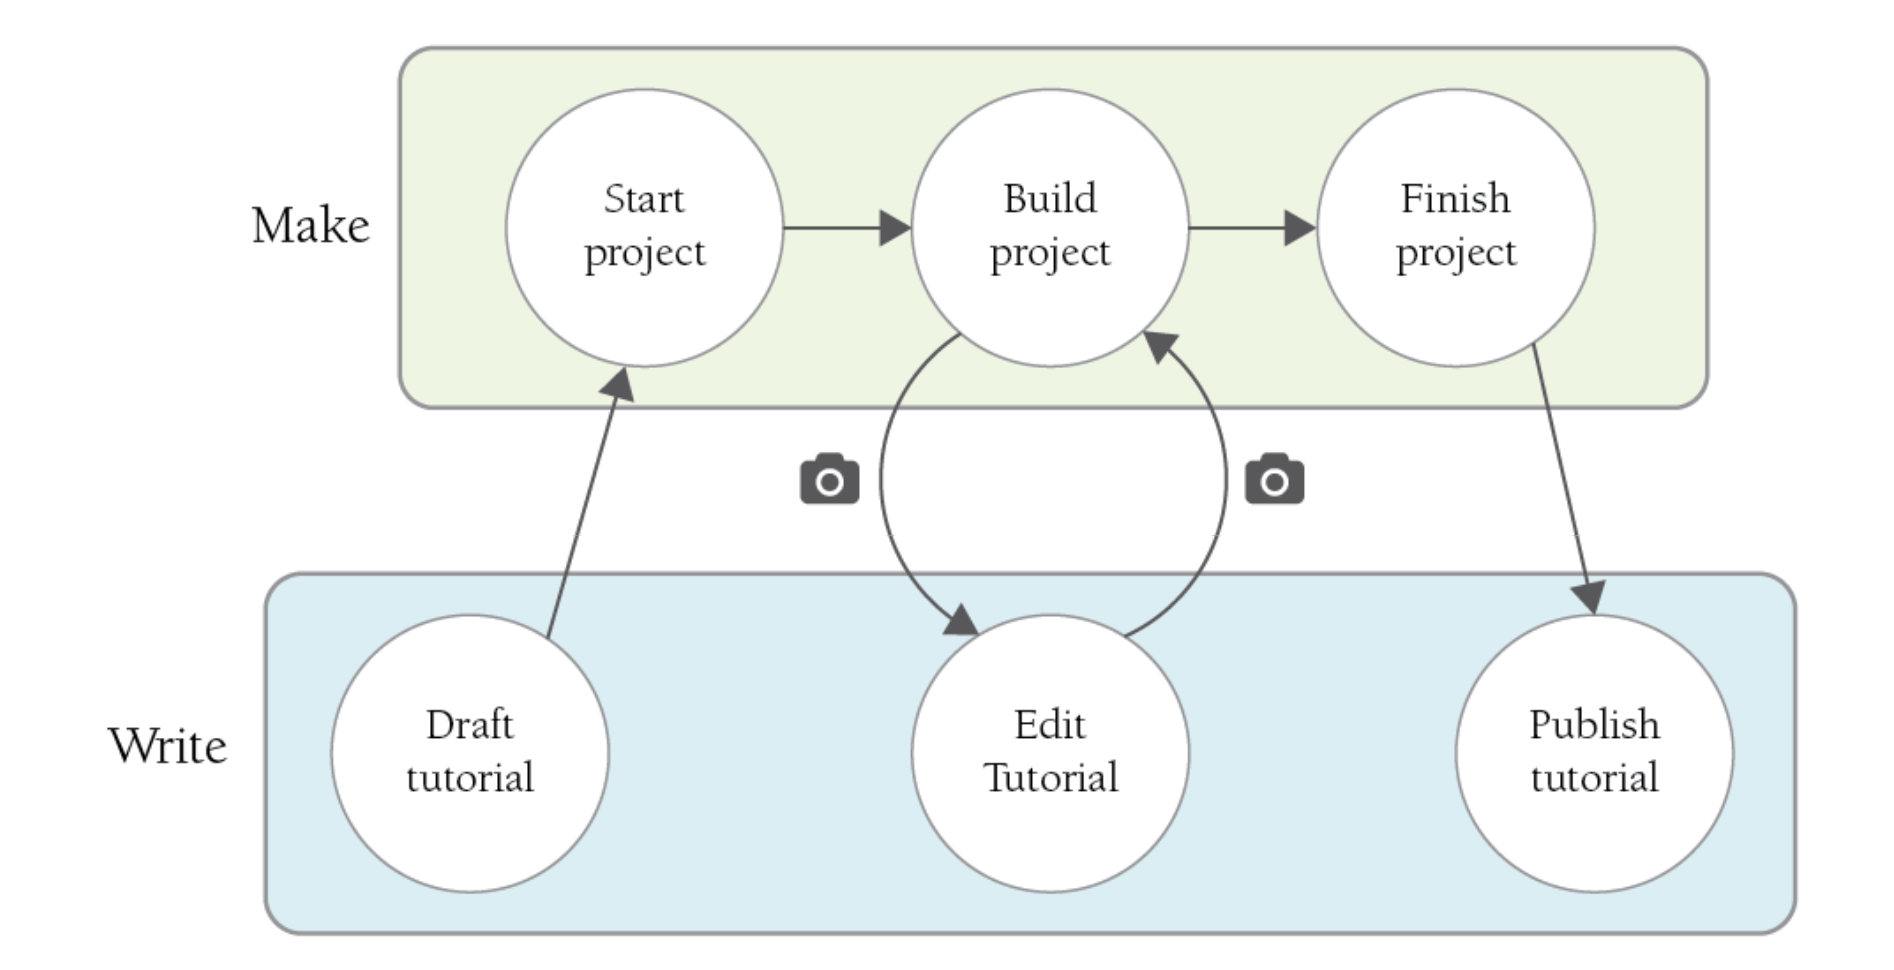
\includegraphics[scale=0.34]{./images/img-makewritesimultanously}
	\caption{First strategy of documenting : write after you make, \cite{tseng2016making}}
	\label{img-makewritesimultanously}
\end{figure}

In summary, the study showed that users need to encapsulate the collected photos and videos to show to create all the steps and a common challenge was to remember to document after each step otherwise users had to replicate their project merely to creating good documentation. 

Finally, authors saw that documentation well worth the effort to share their work but it is time consuming process when a project get more complex, it is hard to follow up or complete the documentation. \cite{scholar:Wakkary:2015:TAH:2702123.2702550}

\subsection{Design and process oriented documentation}
Several approaches were suggested by to improve the online documentation. Documentation techniques requires authors to simultaneously switch between making and writing, make a design process to not miss a step from not being documented or to radically recreate the project to document it in a proper way. Another challenges of documentation technique that needed to support not only the capture of digital artifacts but also physical artifacts where it is not possible to show the physical effort. 
With the recurring need to balance manual and automated ways of capturing, software and hardware tools need to solve open questions and be customizable for different activities and different audiences \cite{Kuznetsov:2010:REA:1868914.1868950}. The workflow of documentation over time needed to not miss a key step in the documentation. 

Documentation process seems to be more important for readers as it give them the opportunity to enable better decision making about components or materials to use \cite{scholar:sf1241364}, as well as successful in encouraging independent exploration and fostering a sense of accomplishment \cite{scholar:lovell2010sewing}. Also, as many users start by replicating some projects, having tools where they could be able to contribute to a project, can help more socializing and boost a collaborative work in the community. 
\section{Build in Progress}

\begin{comment}
\chapter{Experience with a Documentation Platform: from Build-in-Progress to SDG-in-Progress}
\end{comment}

\begin{center}
	\begin{minipage}{.7\textwidth}
		\textit{In this section, I share with you an analyses of how users create and share \textit{DIY} projects via online platform called \textit{SDGinProgress} that we adapted for the SDG sustainable goals, it is a fork from a platform called \textit{BuildinProgress} that focus on maker community like Electronics, food and living. I share findings of two experiences that has been done with 22 student from the Geneva-Tsinghua summer school students and 26 student from the master of University of Geneva, the master is dedicated for the SDG goals. Also I share with you the analyses of this platform and the understanding of how authors and users use it}
	\end{minipage}
\end{center}
%\hl{What is it ?} \hl{Who use it ?} \hl{User interactions ?} \hl{Limitations} \hl{Advantages ?} \hl{Examples ?}
\section{Introduction}
\todo[inline]{Introduction about SDG in Progress, its context and why}

\section{Users Project}
\todo[inline]{mention that the project of Bip was about living etc,, mention some statistics in terms of users projects as well as more qualitaativey type of project.}

\section{features of BiP}
\todo[inline]{what makes BIP different from others.}

Build in Progress is a platform for sharing the story of your design process, where \textit{"makers share how their DIY projects evolve over time}" \cite{tseng2016making}. It focus more on the storytelling of \textit{DIY} documented project, a snapshot of the platform displayed in the figure \ref{img-buildinprogress}. \textcolor{red}{In our experience we forked the platform and we adapted it for the SDG goals, SDGinPRogress consist of 4 parts, (1) Projects where all the project are listed (2) Colllections where featured project are displayed and that depends on their potential (3) welcome page where on the right side you have the list of the 17 SDG goals and undear of each goals you could find a related project to that goal.}

\section{From Build in Progress to SDGinProgress}
\todo[inline]{What we did to go from Build in progress to sdg and the purpose from that move}

SDGinProgress was launched in 2017 and within a collaboration with univeristy of Geneva and the Geneva-Tsinghua summer school, it hosted over 16 projects in categories such as games, environmental project, pollution, digitation all related to an SDG goal.. Users contributed to SDGinProgress community by sharing, providing feedback and describing their progress of each step, the encapsulation of informations lead to a story about the project as SDGinProgress "\textit{support a storytelling approach to documentation}" \cite{tseng2016making}.
\begin{figure}[ht!]
	\centering
	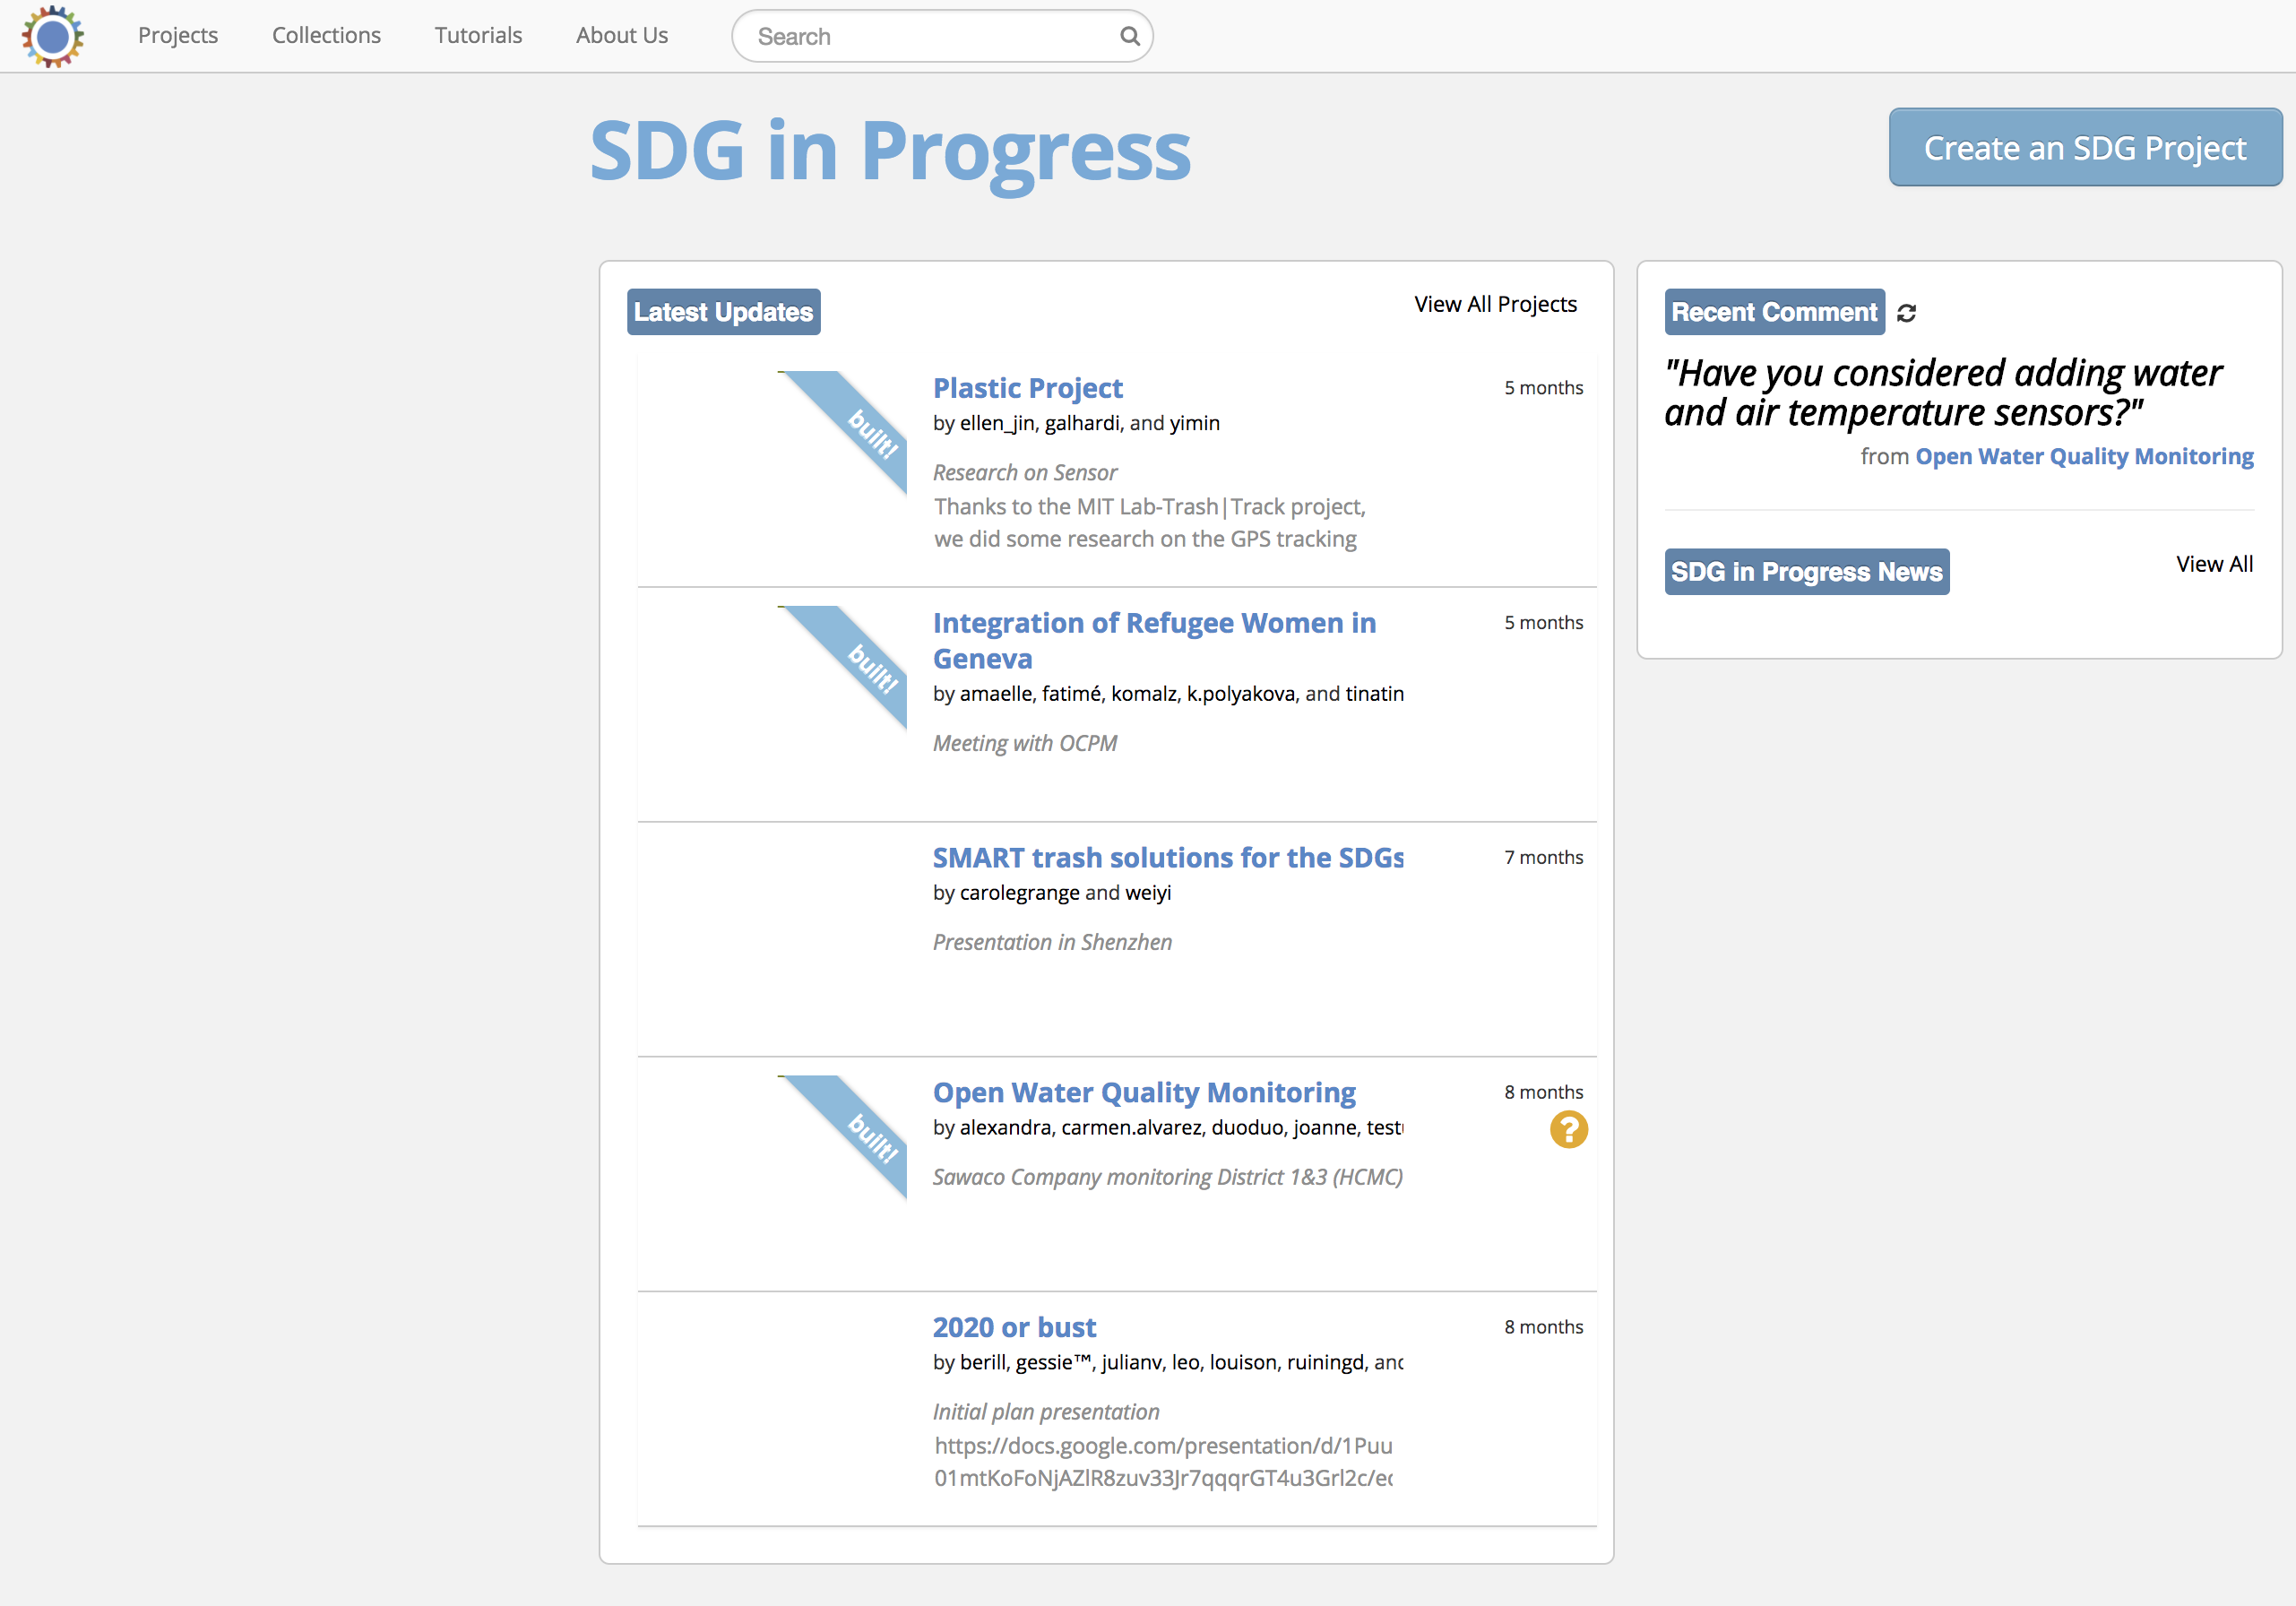
\includegraphics[width=15cm, height=10cm]{./images/img-sdginprogress.png}
	\caption{Build in progress welcome page}
	\label{img-sdginprogress}
\end{figure}

\subsection{Design approach}
Authors shared an iterative design process in the context of sharing their personal journey by creating step-by-step instructions of their project via the online platform \textit{SDGinProgress} and companion mobile application. Readers contributed by suggesting to makers after publishing their steps, makers benefited from sharing step-by-step instructions over time by taking into account the suggestions of readers.

SDGinProgress was developed based on an innovative design process, it enables users to visualize their documentation in an iterative way. Authors can continuously iterate their building process, share their techniques to help others to reach out others in the community so they can have feedback. A social design process principle was considered among the online community to engage users more, to accumulate knowledge, to learn from others and connect users with same interest as \textit{human-related issues in the form of social ties and knowledge sharing were reported as keys to successful collaboration} \cite{Kotlarsky2005}.

\subsection{Features}\label{sec:feature}
SDGinProgress consists of many features in the project page and social feature. The two core features of the project page are : the \textit{Process Map} and \textit{Step Detail View } (\ref{img-sdginprogressproject}).
\begin{figure}[ht!]
	\centering
	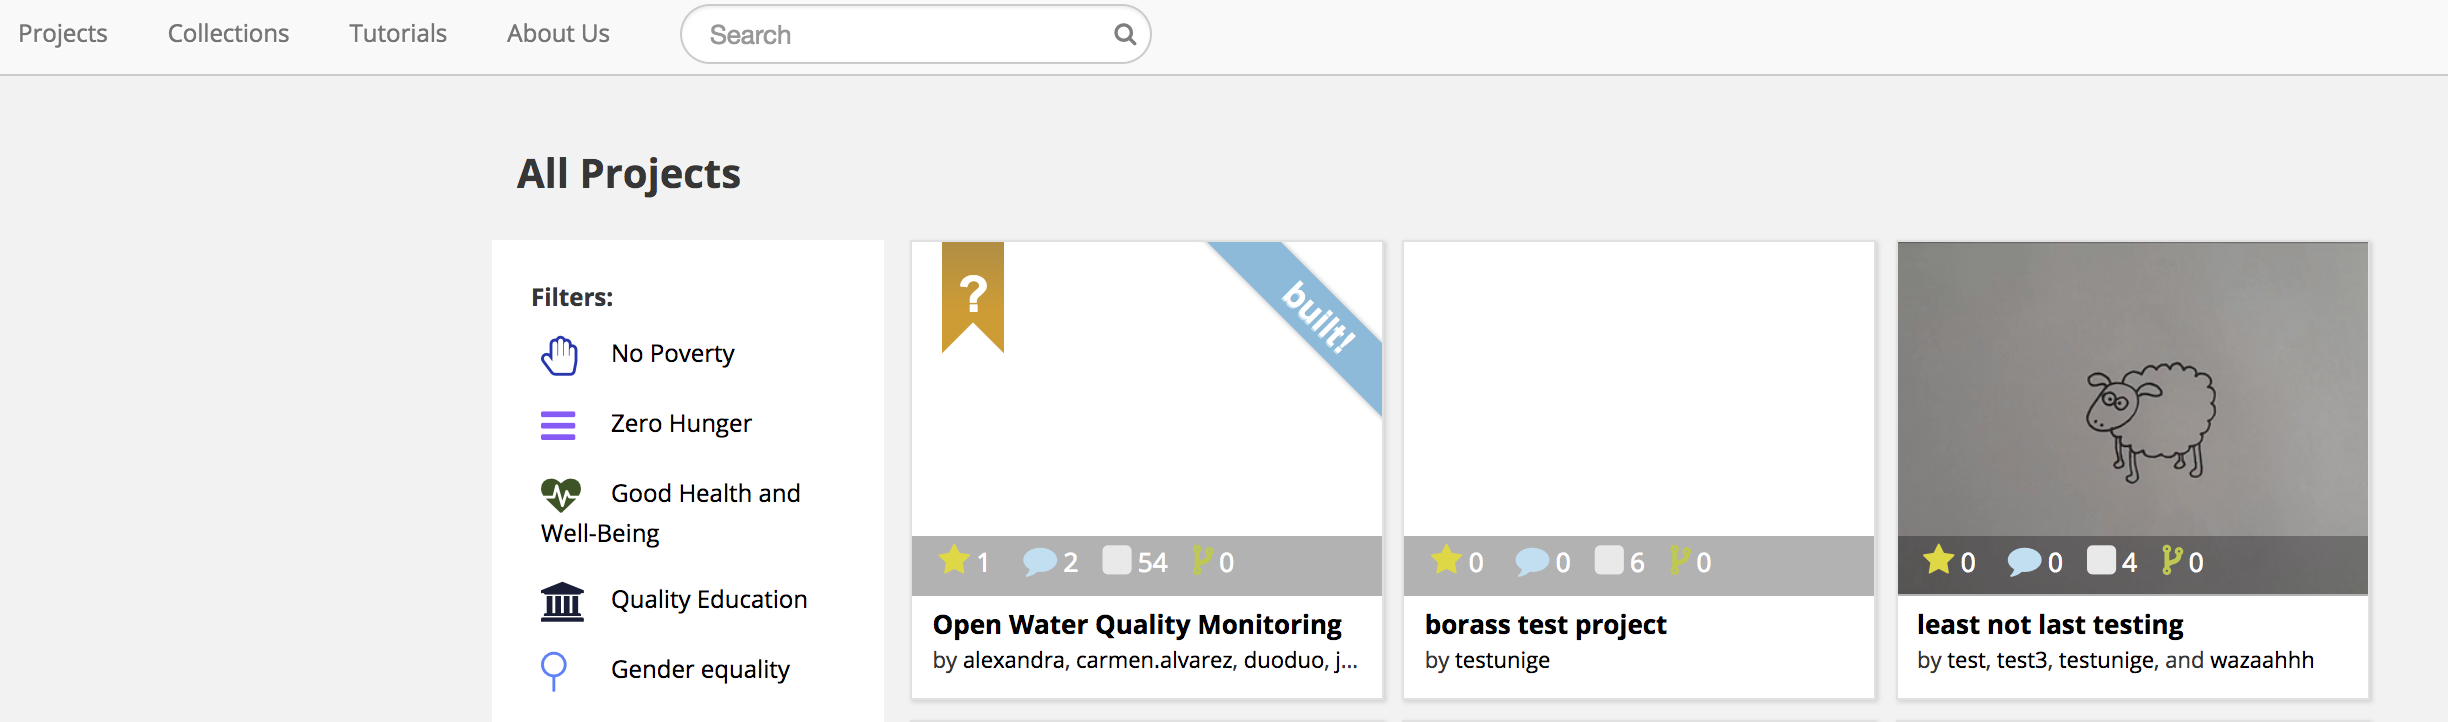
\includegraphics[width=.5\textheight]{./images/img-sdginprogressproject.png}
	\caption{overall project page view, [\url{https://sdginprogress.com/projects/81/steps}]} 
	\label{img-sdginprogressproject}
\end{figure}
In the process map, users can create a step, a label for one or more step, drag \& drop  to rearrange steps. Steps are organized in a tree-map-like format with sui generis branches, a label is added to a branch and it can be colored to designate a branch; for example orange labels represent that a branch is in progress.

Project are displayed in 3 different mode.  The first is the default mode : tree-map, users can go through all the steps, step-by-step and discover more about it as shown in figure \ref{img-viewtreemode1}.
\begin{figure}[H]
	\centering
	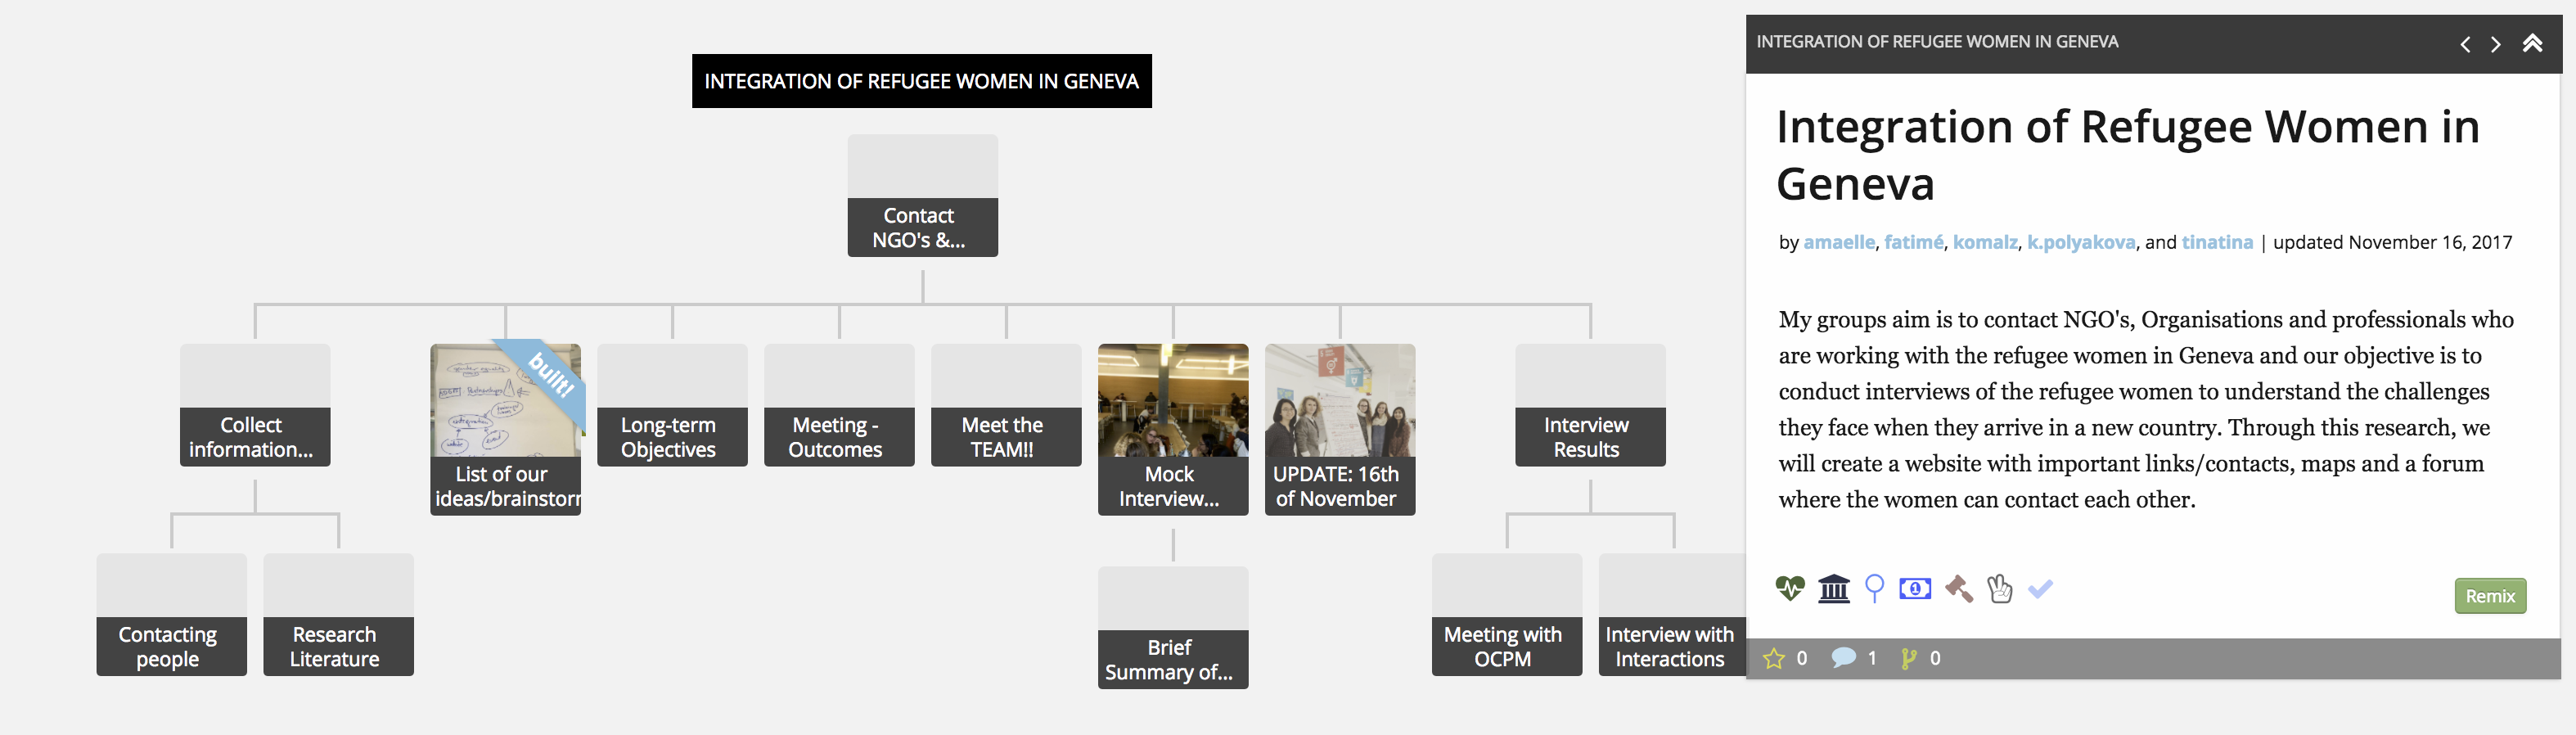
\includegraphics[scale=.25]{./images/img-refugeeintegration.png}
	\caption{tree-map view of the project} 
	\label{img-viewtreemode1}
\end{figure}

The second is Gallery mode \ref{img-viewgallerymode3} and finally  the  blog mode : users can scroll down and an index of steps will be displayed on their left side of the page (figure \ref{img-viewgallerymode3}).

\begin{figure}[H]
	\centering
	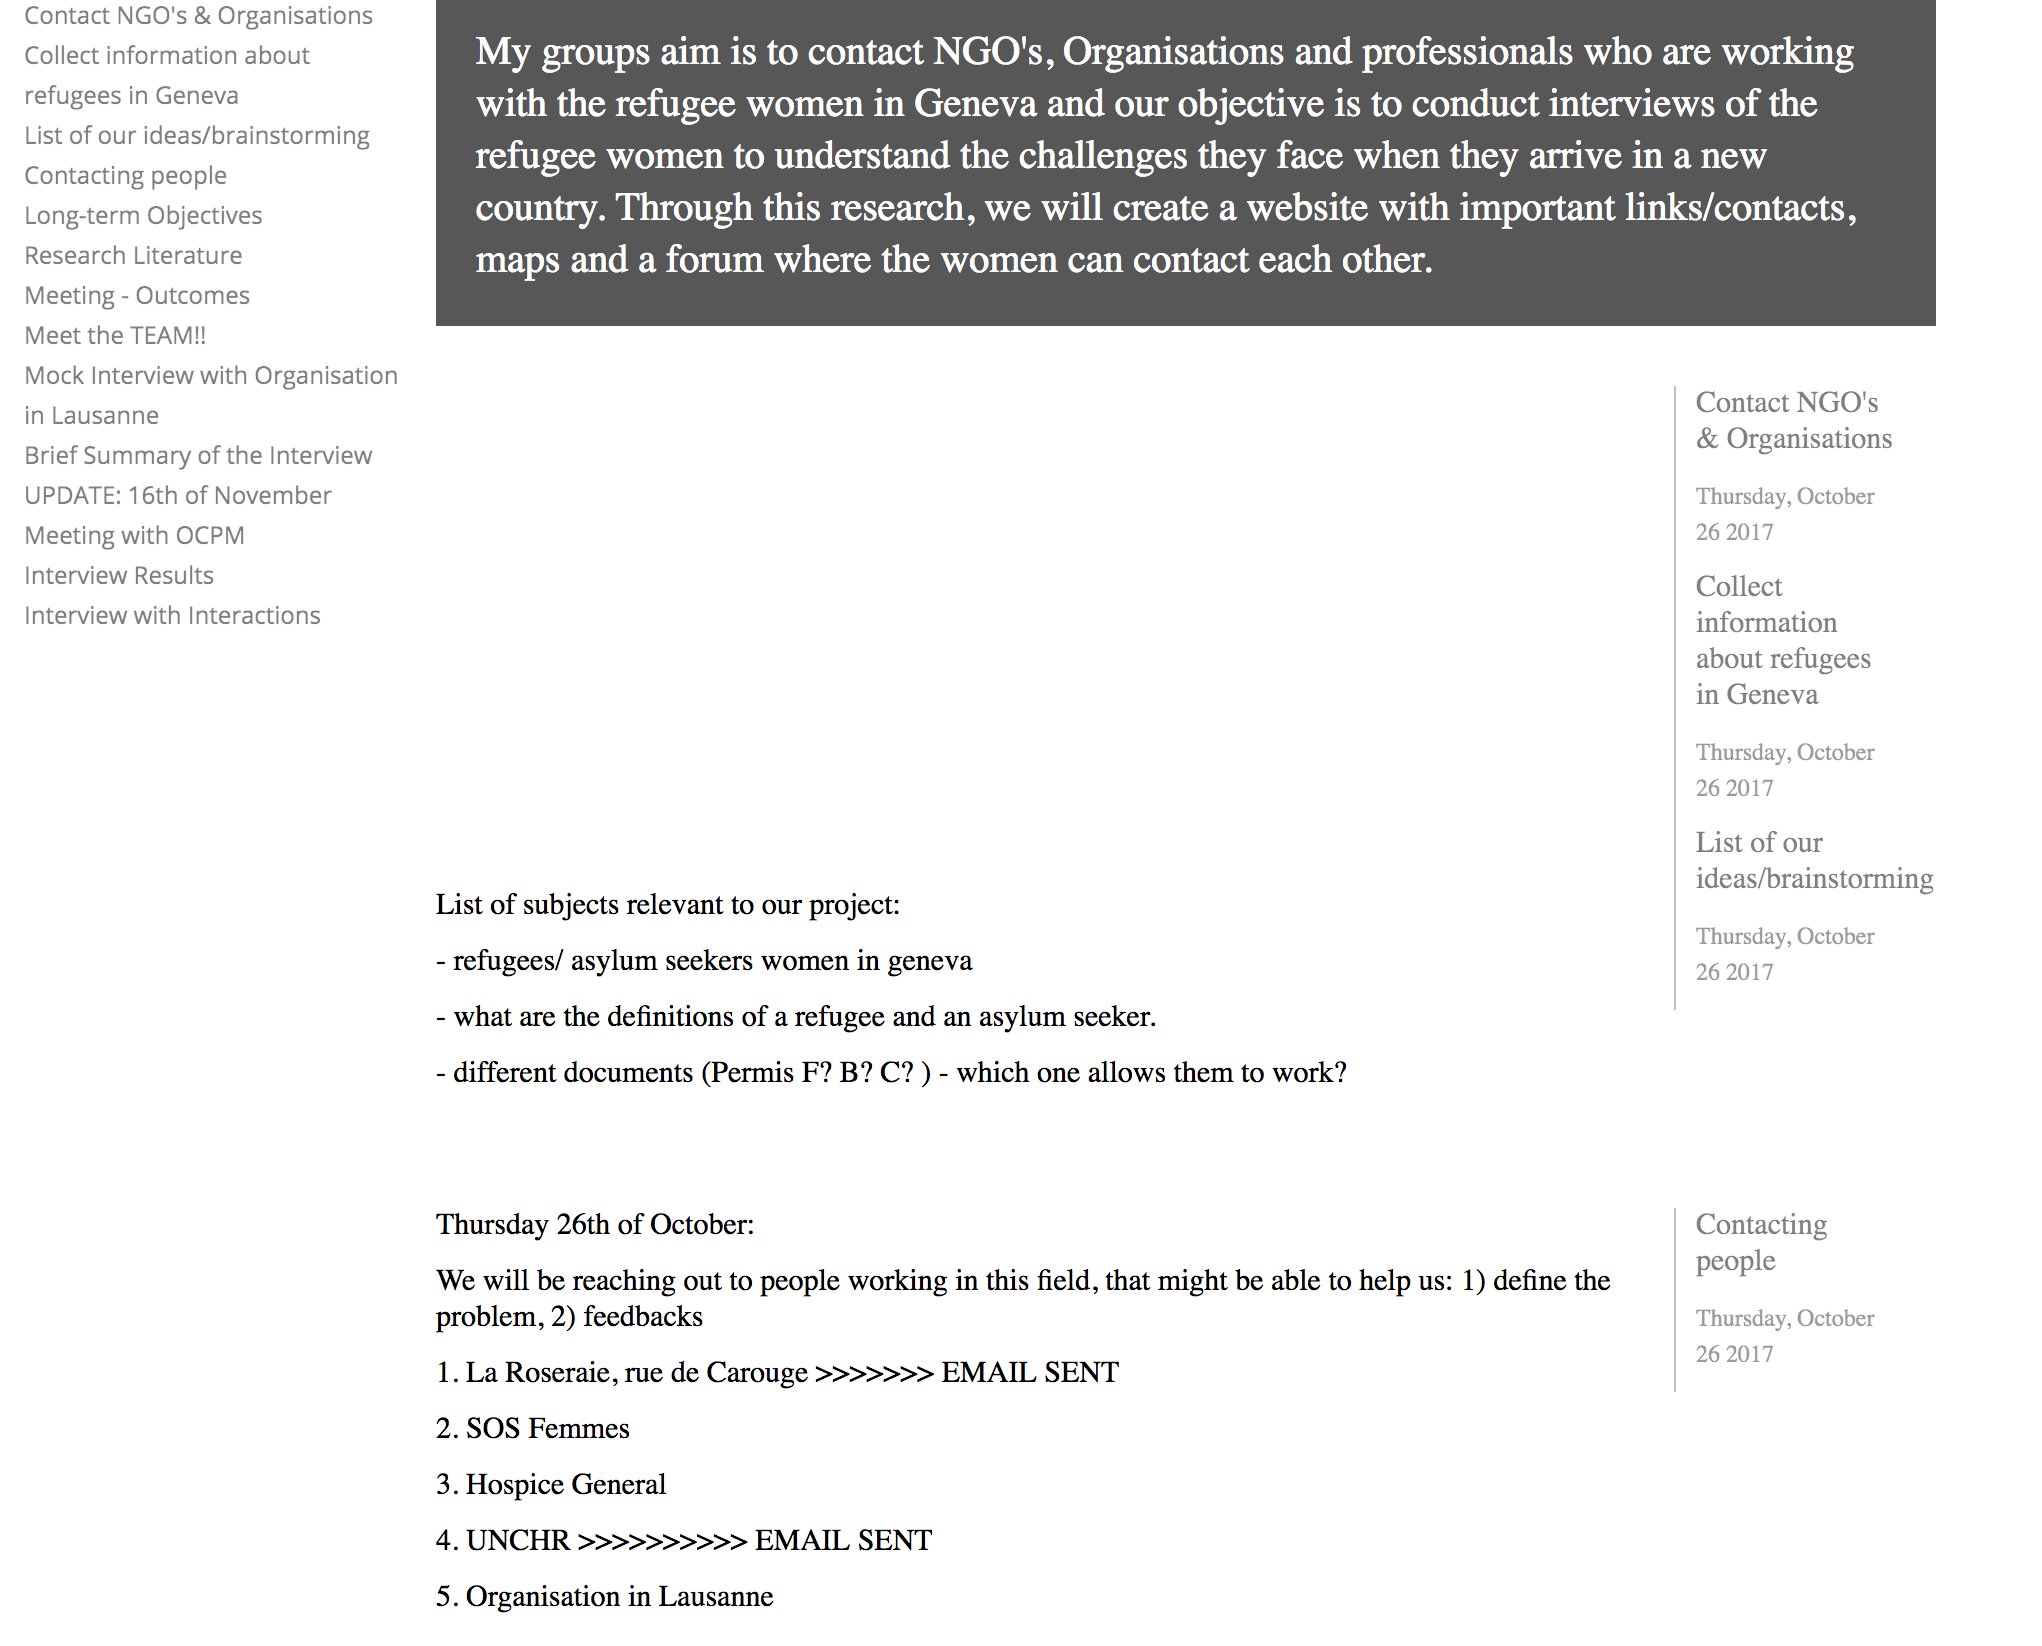
\includegraphics[scale=.3]{./images/img-refugeeintegrationblogmode.png}
	\caption{Gallery view of the project} 
	\label{img-viewgallerymode3}
\end{figure}

%\begin{figure}[H]
%	\centering
%	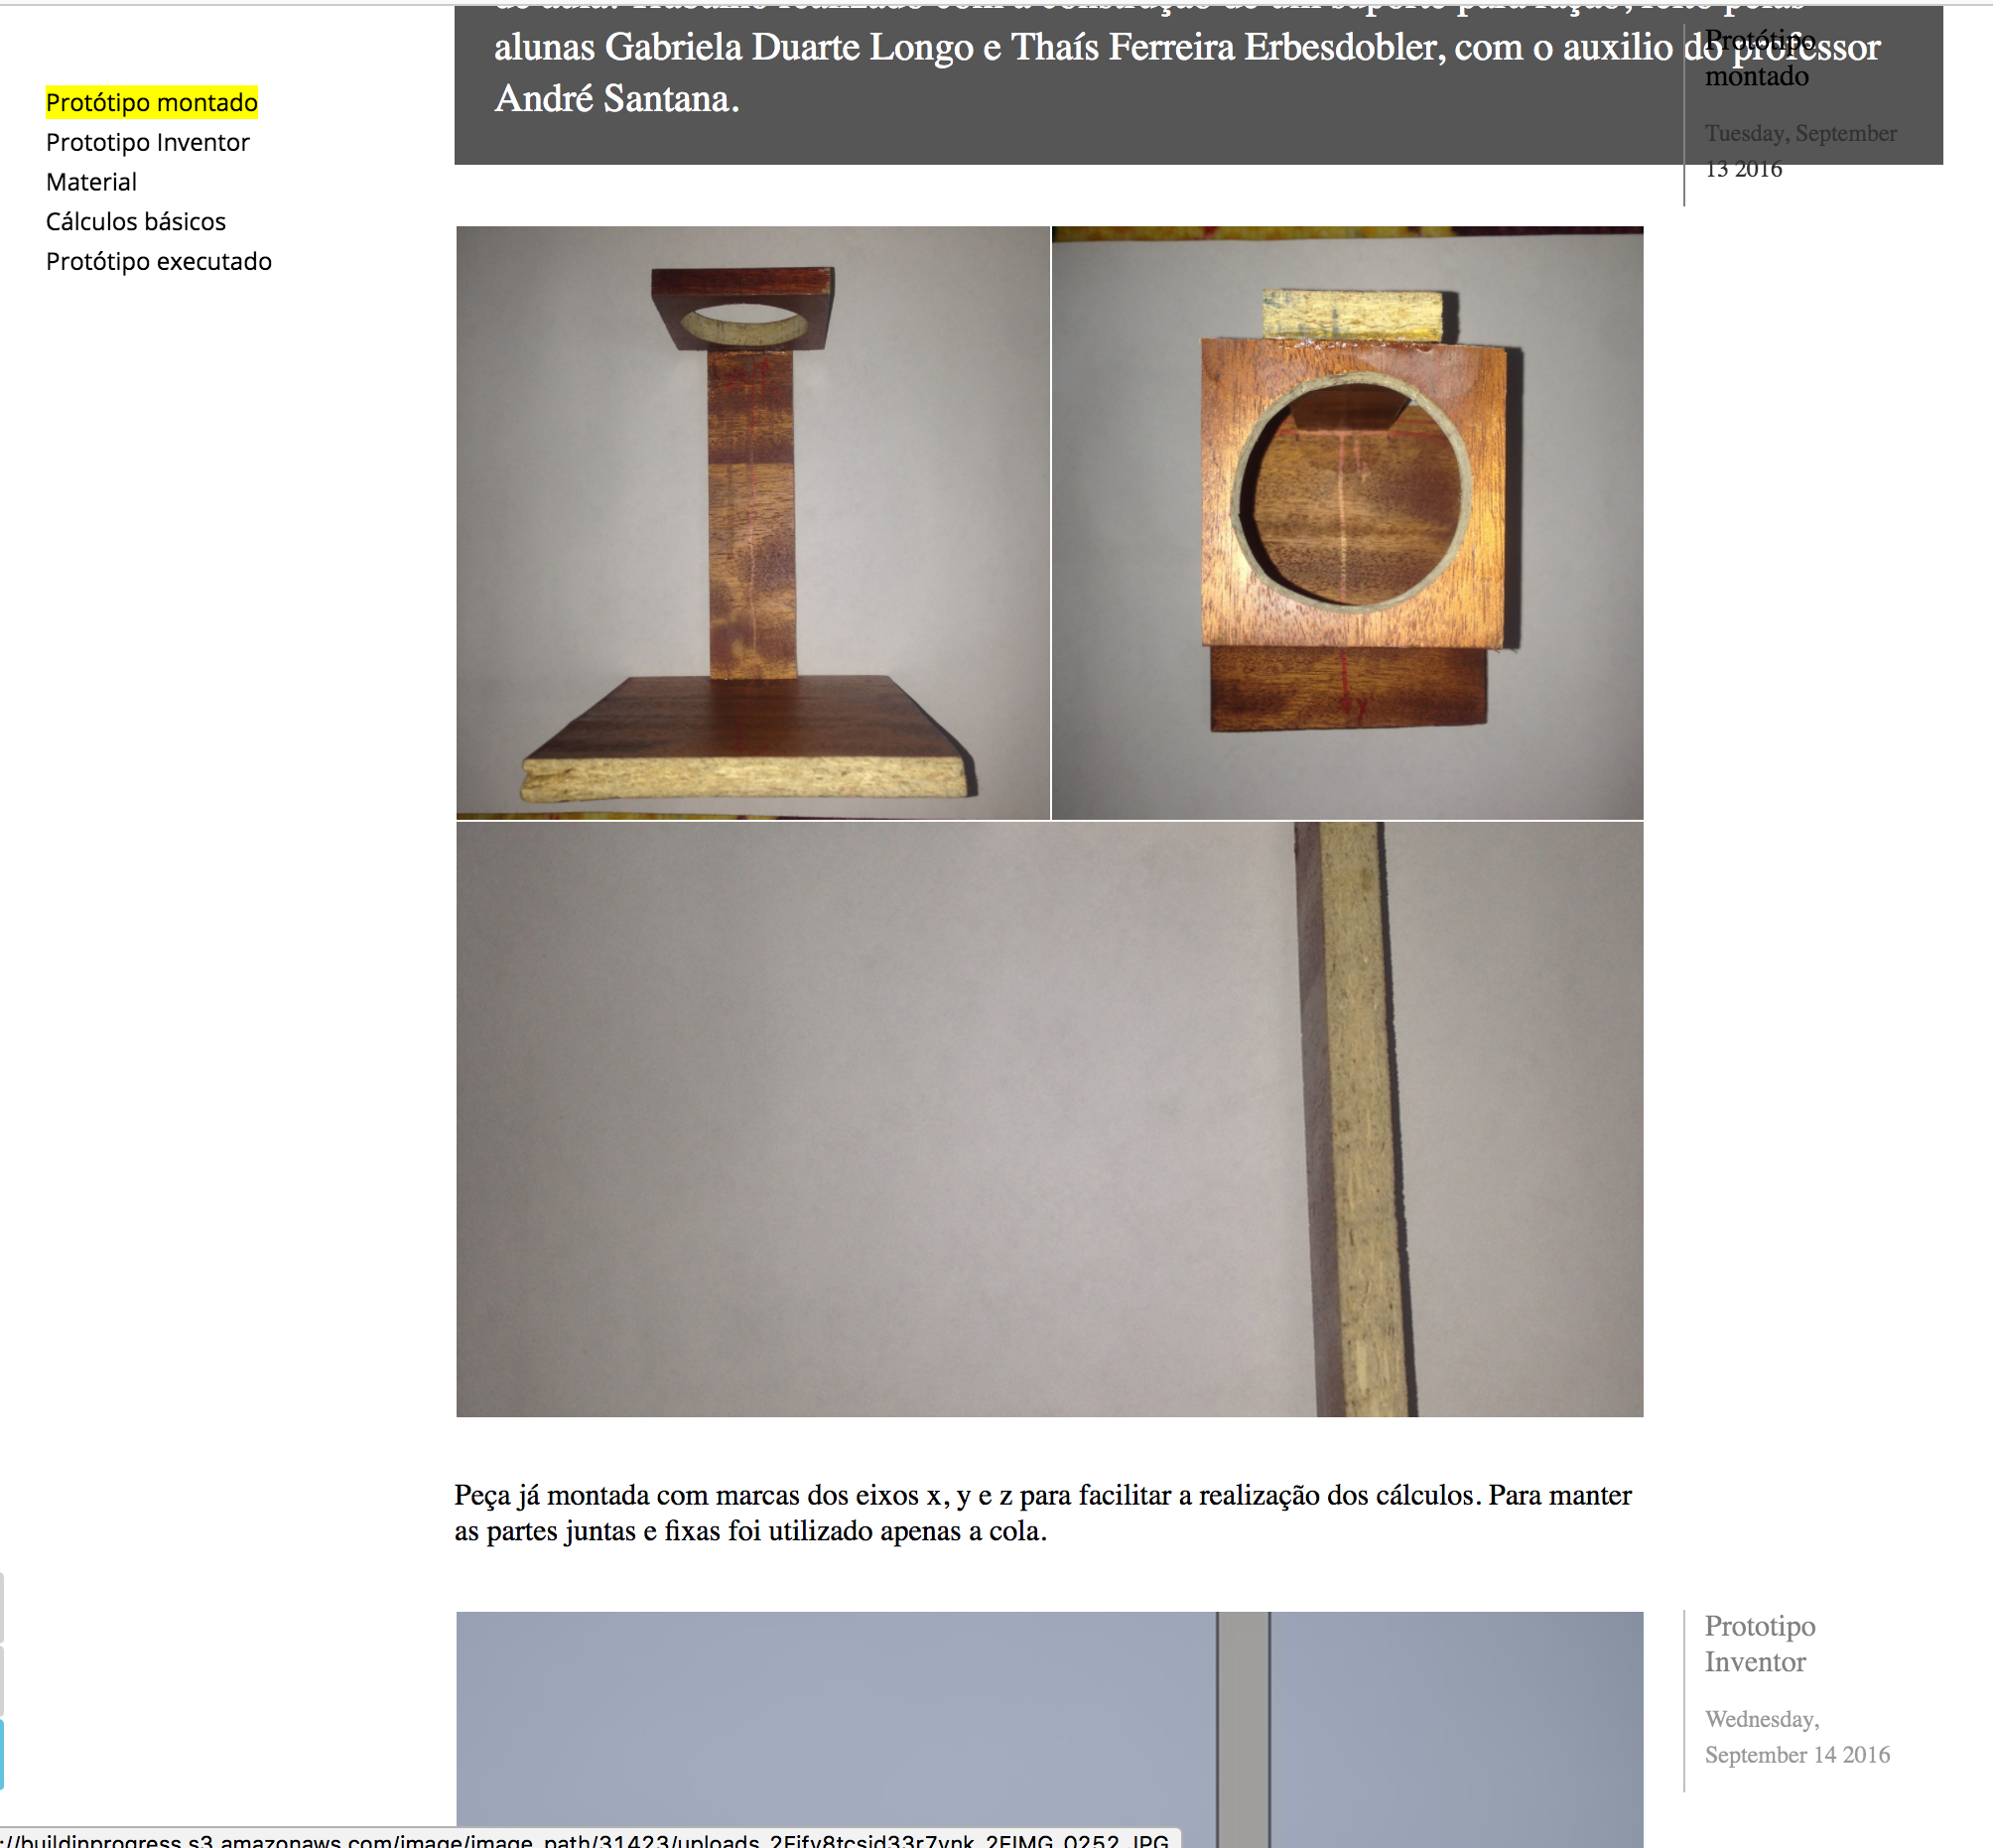
\includegraphics[scale=.3]{./images/img-mode3.png}
%	\caption{Blog like mode} 
%	\label{img-mode3}
%\end{figure}

In \textit{Details of step} users can upload photos or videos, add text description, ask others a question that will appear in the homepage of the platform, upload resources or files in different formats; e.g. .PDF, .PPT, a given example is shown in the figure \ref{img-stepdetails1} .
\begin{figure}[H]
	\centering
	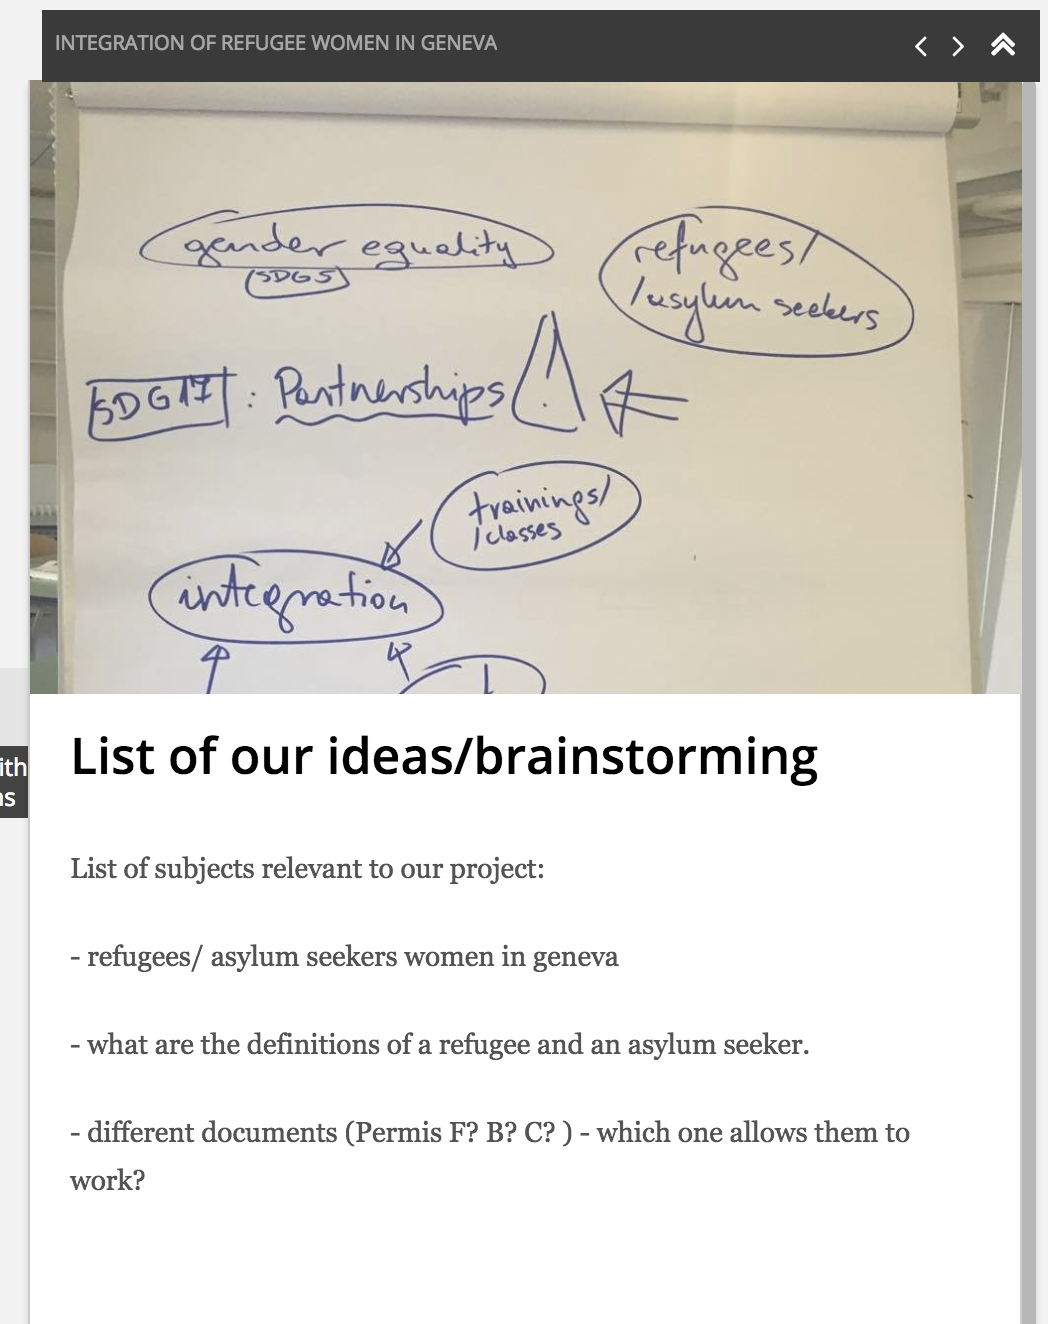
\includegraphics[scale=.3]{./images/img-stepdetails1.png}
	\caption{Details steps view} 
	\label{img-stepdetails1}
\end{figure}

The online platform incorporate many features that keep the SDGinProgress community more socialized and connected. Users can follow a project, see recent activity on the homepage and they will receive notification once an author add a step or ask a question.
\begin{figure}[H]
	\centering
	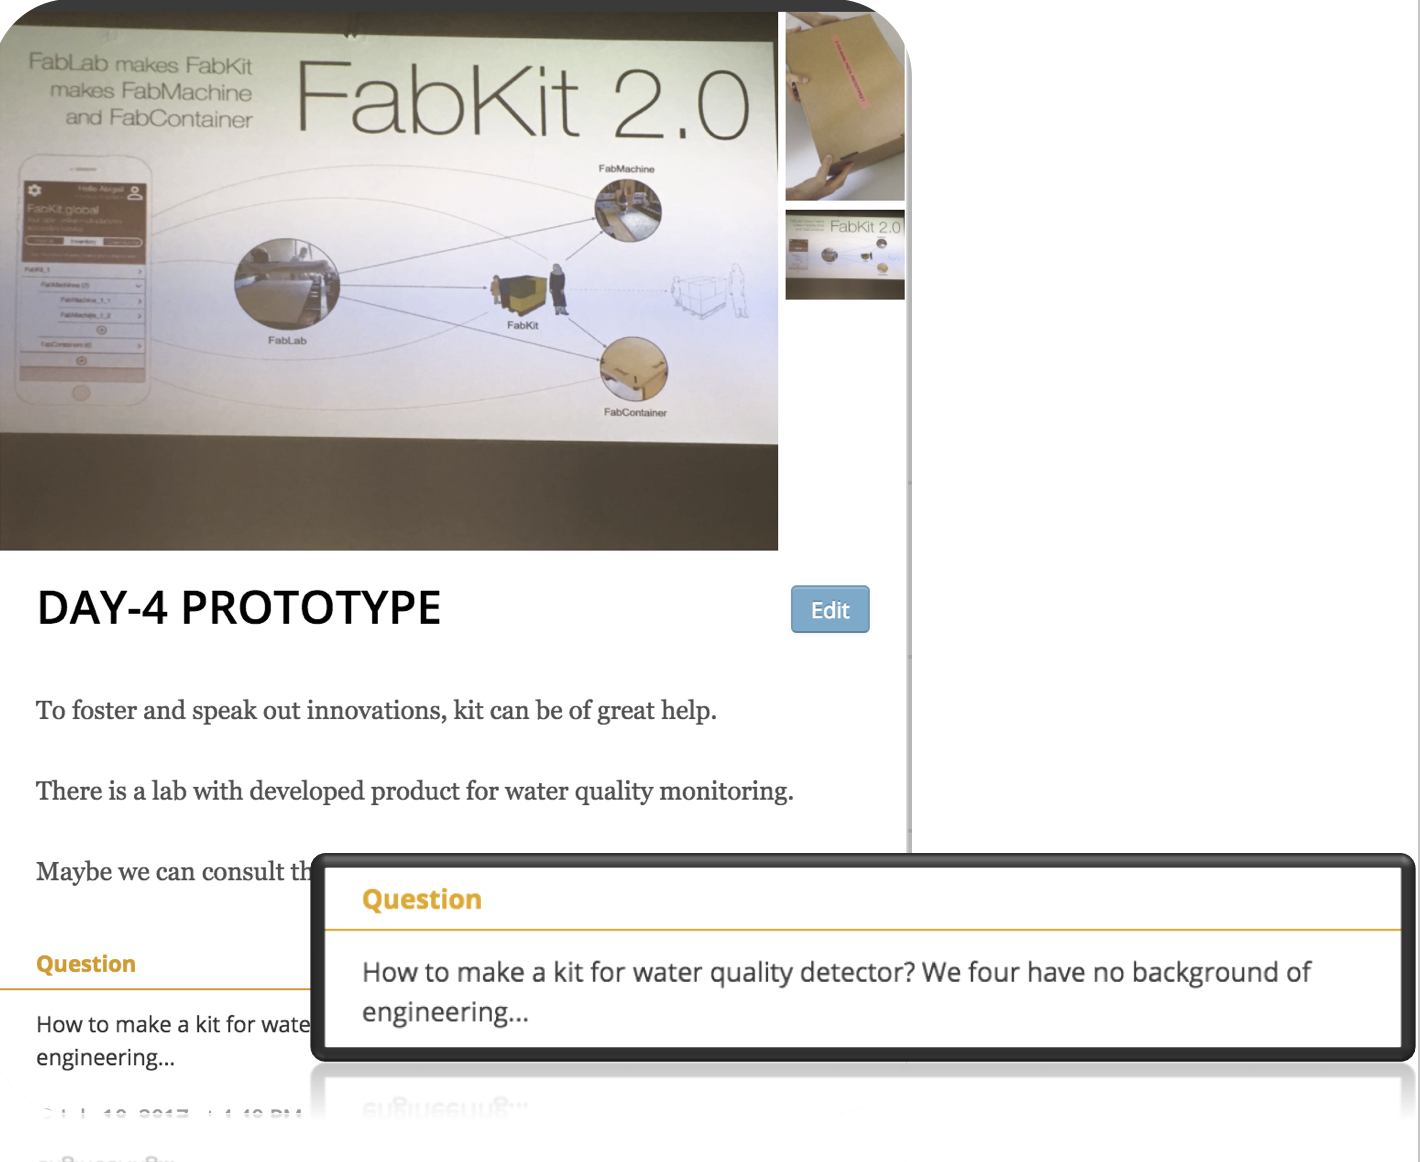
\includegraphics[scale=.4]{./images/img-commentquestion1.png}
	\caption{Question featured in the home page} 
	\label{img-commentquestion}
\end{figure}

Moreover, users can leave a text on any step and they will receive a notification when a comment is left. Authors can ask for feedback or help by embedding a question that will be added to the Community Activity section of the homepage, see figure \ref{img-commentquestion}.
\subsubsection{Mobile application}
A mobile application has been created to make documentation more efficient in which users upload images and videos to their projects directly from their devices instead of taking picture from their devices then transfer it to a computer and upload it (figure \ref{img-mobileapp}). But in our experience with the summer school we didn't used it.
\begin{figure}[H]
	\centering
	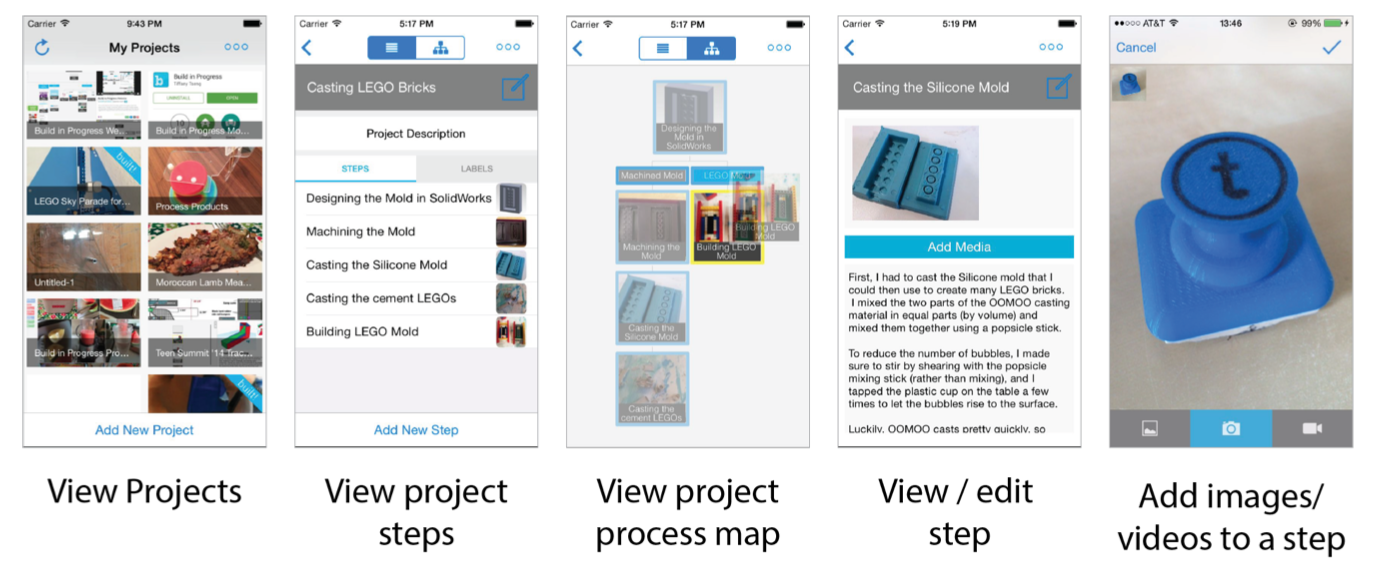
\includegraphics[scale=.5]{./images/img-mobileapp.png}
	\caption{Mobile application interface, [Tseng, 2016]} 
	\label{img-mobileapp}
\end{figure}


\section{Use of SDG}
\todo[inline]{How many teams used it, what they usd it for}
\todo[inline]{Quote some feedback if it is written or recorded}

\subsection{User interaction}
SDGinProgress has been used in summer-school programs and in after-summer-school by students who work on their own project. Teenagers and one adult facilitator have been interviewed and a weekly interview has been done to all teams to get an estimation about their weekly hours work.

The results of the interviews and surveys showed that users get motivated to share their project at the beginning as it facilitate getting a feedback of what they have done, create and show their portfolio projects, get engaged to document and to help others. Users were divided into two opinions, one part of the students found that SDGinProgress support meaningful documentation practices and the second part of the students found that it doesn't support their project the latter are typically software development project or policy making. Many strategies were identified depending on the type of project, the duration of a project and the age of makers who are using it.

\subsection{Summary}

The study of SDGnProgress showed that it support authors and readers but it has some limitation. The documentation help students to create a design process for their project by learning from the many iterations they did over time and SDGnProgress motivates reflective practice on making, design process, and values and identity. Users get engaged, get feedback, and help others. SDGinProgress support all capturing way written and visual. \textcolor{red}{In our experiments} The platform SDGinProgress helped students to document their project and it gaves them the opportunity to win visibility and get feedback from others, for example, as we see in the picture below. 
\begin{figure}[ht!]
	\centering
	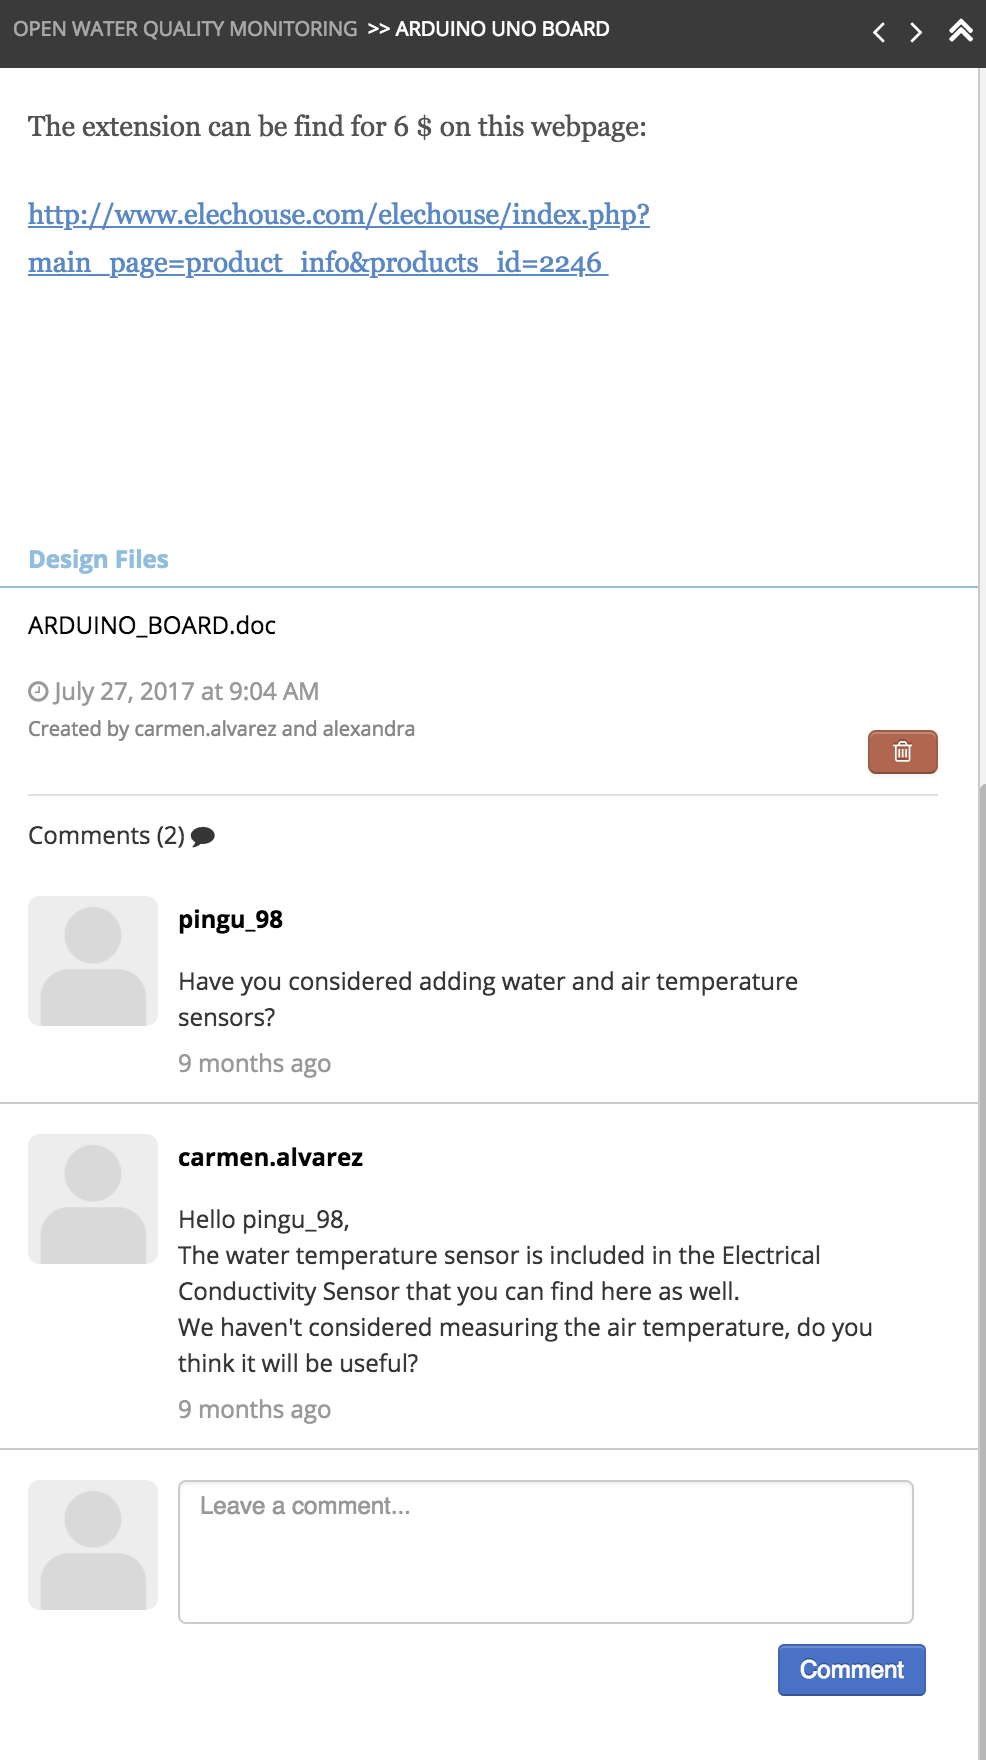
\includegraphics[width=.3\textheight]{./images/img-cmtsdgip.png}
	\caption{Comments and feedbacks on a hardware ste, \cite[\url{https://sdginprogress.com/projects/47/steps?comment_id=4&notification_id=442&step=214}]{SDGdinP1}} 
	\label{img-cmtsdgip}
\end{figure}
An engineer from CERN is giving them a comment about their hardware, others were asking question to the public to get some ideas. so the use of the platform overall is good for documentation but there is a lack of incentive for writing. Student tend to postpone documentation then forget what they want to document, which lead to weak documentation that give the big outline about a project and it doesn't really help if someone else want to copy the project






\section{Discussion}

\textit{SDGinProgress} and \textit{Instructables} didn't bring a new fundamental way in which users can share their captured media publicly or in private. Design parameters can be adjusted to support different type of users-interactions and goals.  Instructables enable users to personalize through substitution and modification of a step and any missing step mean that authors should re-create their documentation while BiP focus more on the  design process where users can iterate their project by creating new branches and forget about the unsuccessful branches.

The mix between capturing and text-based-description features in SDGinProgress enables teenagers to document. The ease of use for creating a branch, drag \& drop simplify the job for younger audience especially readers who are new to the community of \textit{DIY} as they can go through steps, iterate on their work, modify a step or re-arrange some steps.  Instructables has both features but there is no friendly structure where authors get their documentation organized and if an author has a limited background in documentation or he doesn't like it, he will probably abandon the documentation of a project after the first type a user find that it is not possible to re-arrage the documented steps.

Sharing a project is not enough for authors. Users in Instructables found that they cannot share their thought or it is limited as the only way to express what they think is via a comment. SDGinProgress offers a text-based option where both authors and readers could ask a question or leave a comment, also, both can receive a notifications for a reply from the community or any other news concerning any modification in the project.

The process of sharing the effort in progress enable users to communicate more in BiP, they helped each other, they showed their effort, they get featured and receive feedback as described in section \ref{sec:feature}. Balancing the ease of use of automated documentation systems with the powerful feature, a mobile application, encourage more users to upload pictures or videos and enable them to be physically free so they can move around to document their project for example without having the problem of taking a photo, remember which step it is, transfer it then upload it to the platform as in Instructables.




\chapter{Challenge Based Event}

\section{Timeline of event}
Visual for the timeline of events
When it starts, when it ends, what happened in between and after

\section{Test of CBE : Summer school}
\chapter{Summer School}

\subsection{Summer school projects}
\label{sec:scprojects}
Summer school is 8 week, 6 weeks in Geneva, 2 weeks in China.
Student are supposed to tackle SDG problem.
work on their idea in the first 8 weeks then go to China to prototype it using the facilities and the expertise that exist there.


\subsection{Summer school teams}
\label{sec:scteams}
4 teams A and B

2 document as they want

2 document as suggested from the coach

2 patterns finded, vertical documentaiton  and horizontal documentation


Vertical documentation, teams who document in a timeline whatever step they do without any label considering this, like week 1, week 2 as you see in the picture belo

Horizontal documentation : teams started to document vertical way, then we gave them a template to document.
to them how they could document in a way where their followers could take a project from them and they started to devide their documentation into litterature, hardware, software testing, brainstorming

We asked a team to document via github.





\subsection{Summer school documentation}
There are around 9 project documented in this platform
we asked 24 student to read these project and write a feedback about it and see if they could pick up a project from it.
Zero project was selected, why ?
first EGO. 
Second: documentation they don't find it useful, there are a missing part of the documentation like the litterature, benchmarking, few people knows how to do the benchmarking and I think this is a key in documentation,  to read with openess, everyone has its own way of writing and documenting and they need to be open for others idea to write 
\label{sec:scdocumentation}
\section{Test of CBE : HUG hack}

\section{Events documentation}

How events are documented

Hug hack
mobility hack
the port
sc
ms


\section{Efforts}
Visual of human resources 

\chapter{CBE documentation : Case study}

\section{Adaptation of BIP}

\section{Motivation}

\section{Data set :  SDGinProgress}

Number of project, 
Number of boxes,
Number of comments,
Number of questions,
Number of answers,

Survey : 
\begin{itemize}
\item What do you use to document your project ?
\item What do you use to communicate ?
\item what do you use to share folders ?
\item what do you use to present/show what you did ?
\end{itemize}
\section{Feedback from project}

Why you didn't take any project SDG

\chapter{Discussion}
Successful documentation from 

1- China (carols project)
2- CosmicPi 

\chapter{Conclusion and Recommendation \& Future Work}

\begin{itemize}
	\item In which case it will make sens to use SDG in Progress
	\item Software perspective what could be done 
	\begin{itemize}
		\item what it does
		\item how it works
		\item software side
		\item interface
		\item how we adapt it for each type of events
		\item -- what is the challenge that we face 
		\item how to motivated people to document easly
		\item -- incetive of documentation
		\item documentation is positive outcome
	\end{itemize}
	\item Competitor
	\item Visual about instream of documentation
	\item Outstream ?
\end{itemize}


Innovators need tools for documentation to support their innovations. We found that one tool is not enough to support different goals and types of interactions especially if users are from different background and ages. But the availability of features in some tools can enable users to fulfil their need either in showing their effort, keeping tracks of their ideas \cite{Wakkary:2015:TAH:2702123.2702550}, sharing their experience or exchange knowledge \cite{doi:10.1287/orsc.1070.0325}. 

In this state-of-the-art we analysed \textit{Instructables} the most popular online community for \textit{DIY} and the most recent \textit{DIY} platform \textit{BuildinProgress} but at the same time I went through many other online community \textit{Dorkbot, Ravelry, Craftster, Etsy, hacker, hackster.io} and I found that \textit{DIY} community share one need : A tool that enable makers, hackers and innovators to share their experiences in  a proper and meaningful ways.  Another thing I have learned from my experience of more than 13 hackathons, the analyses of \textit{Instructables}  and \textit{BiP} is that developing a new tools will not bring a new fundamental way of capturing media or writing text for documentation. Eventually, a goal would be to improve the process map used in SDGinProgress. 

I can conclude that an existing tool is needed from a wide range of \textit{DIY} community that would enable them to document in a meaningful way and make their documentation more sustainable. I believe, a tool that contains all necessary features for documentation with enhanced design process could be the new popular tool to use by \textit{DIY} community to document their effort in meaningful ways. To prove this we need to see how innovators will use this tool, how useful it would be and the method of design process would be questioned.


\textcolor{red}{
	\section{Future work}
	1- Study the open geneva experience for the next 5 years
	2- Understand the incentive of writing from participants and build a tool that could fill the gap of documentation
	3- Build a robo doc that could be part of a team, talk to them, collect data and help them documenting
	4- Study the difference  the instream of hackathons (why more and more industry are getting in )and look at the outstream of hackathon and how it could be stimulated.}

\chapter{Platform analyses} 


\section{Instructable}


\begin{center}
	\begin{minipage}{.7\textwidth}
		\textit{In this section, I share with you an analyses of how users create and share \textit{DIY} projects via online platform called Instructables. I share findings of the analyses of this platform and the understanding of how authors and users use Instructables}
	\end{minipage}
\end{center}

\begin{comment}
\hl{What is it ?} \hl{Who use it ?} \hl{User interactions ?} \hl{Limitations} \hl{Advantages ?} \hl{Examples ?} \\
\end{comment}

\begin{figure}[ht!]
	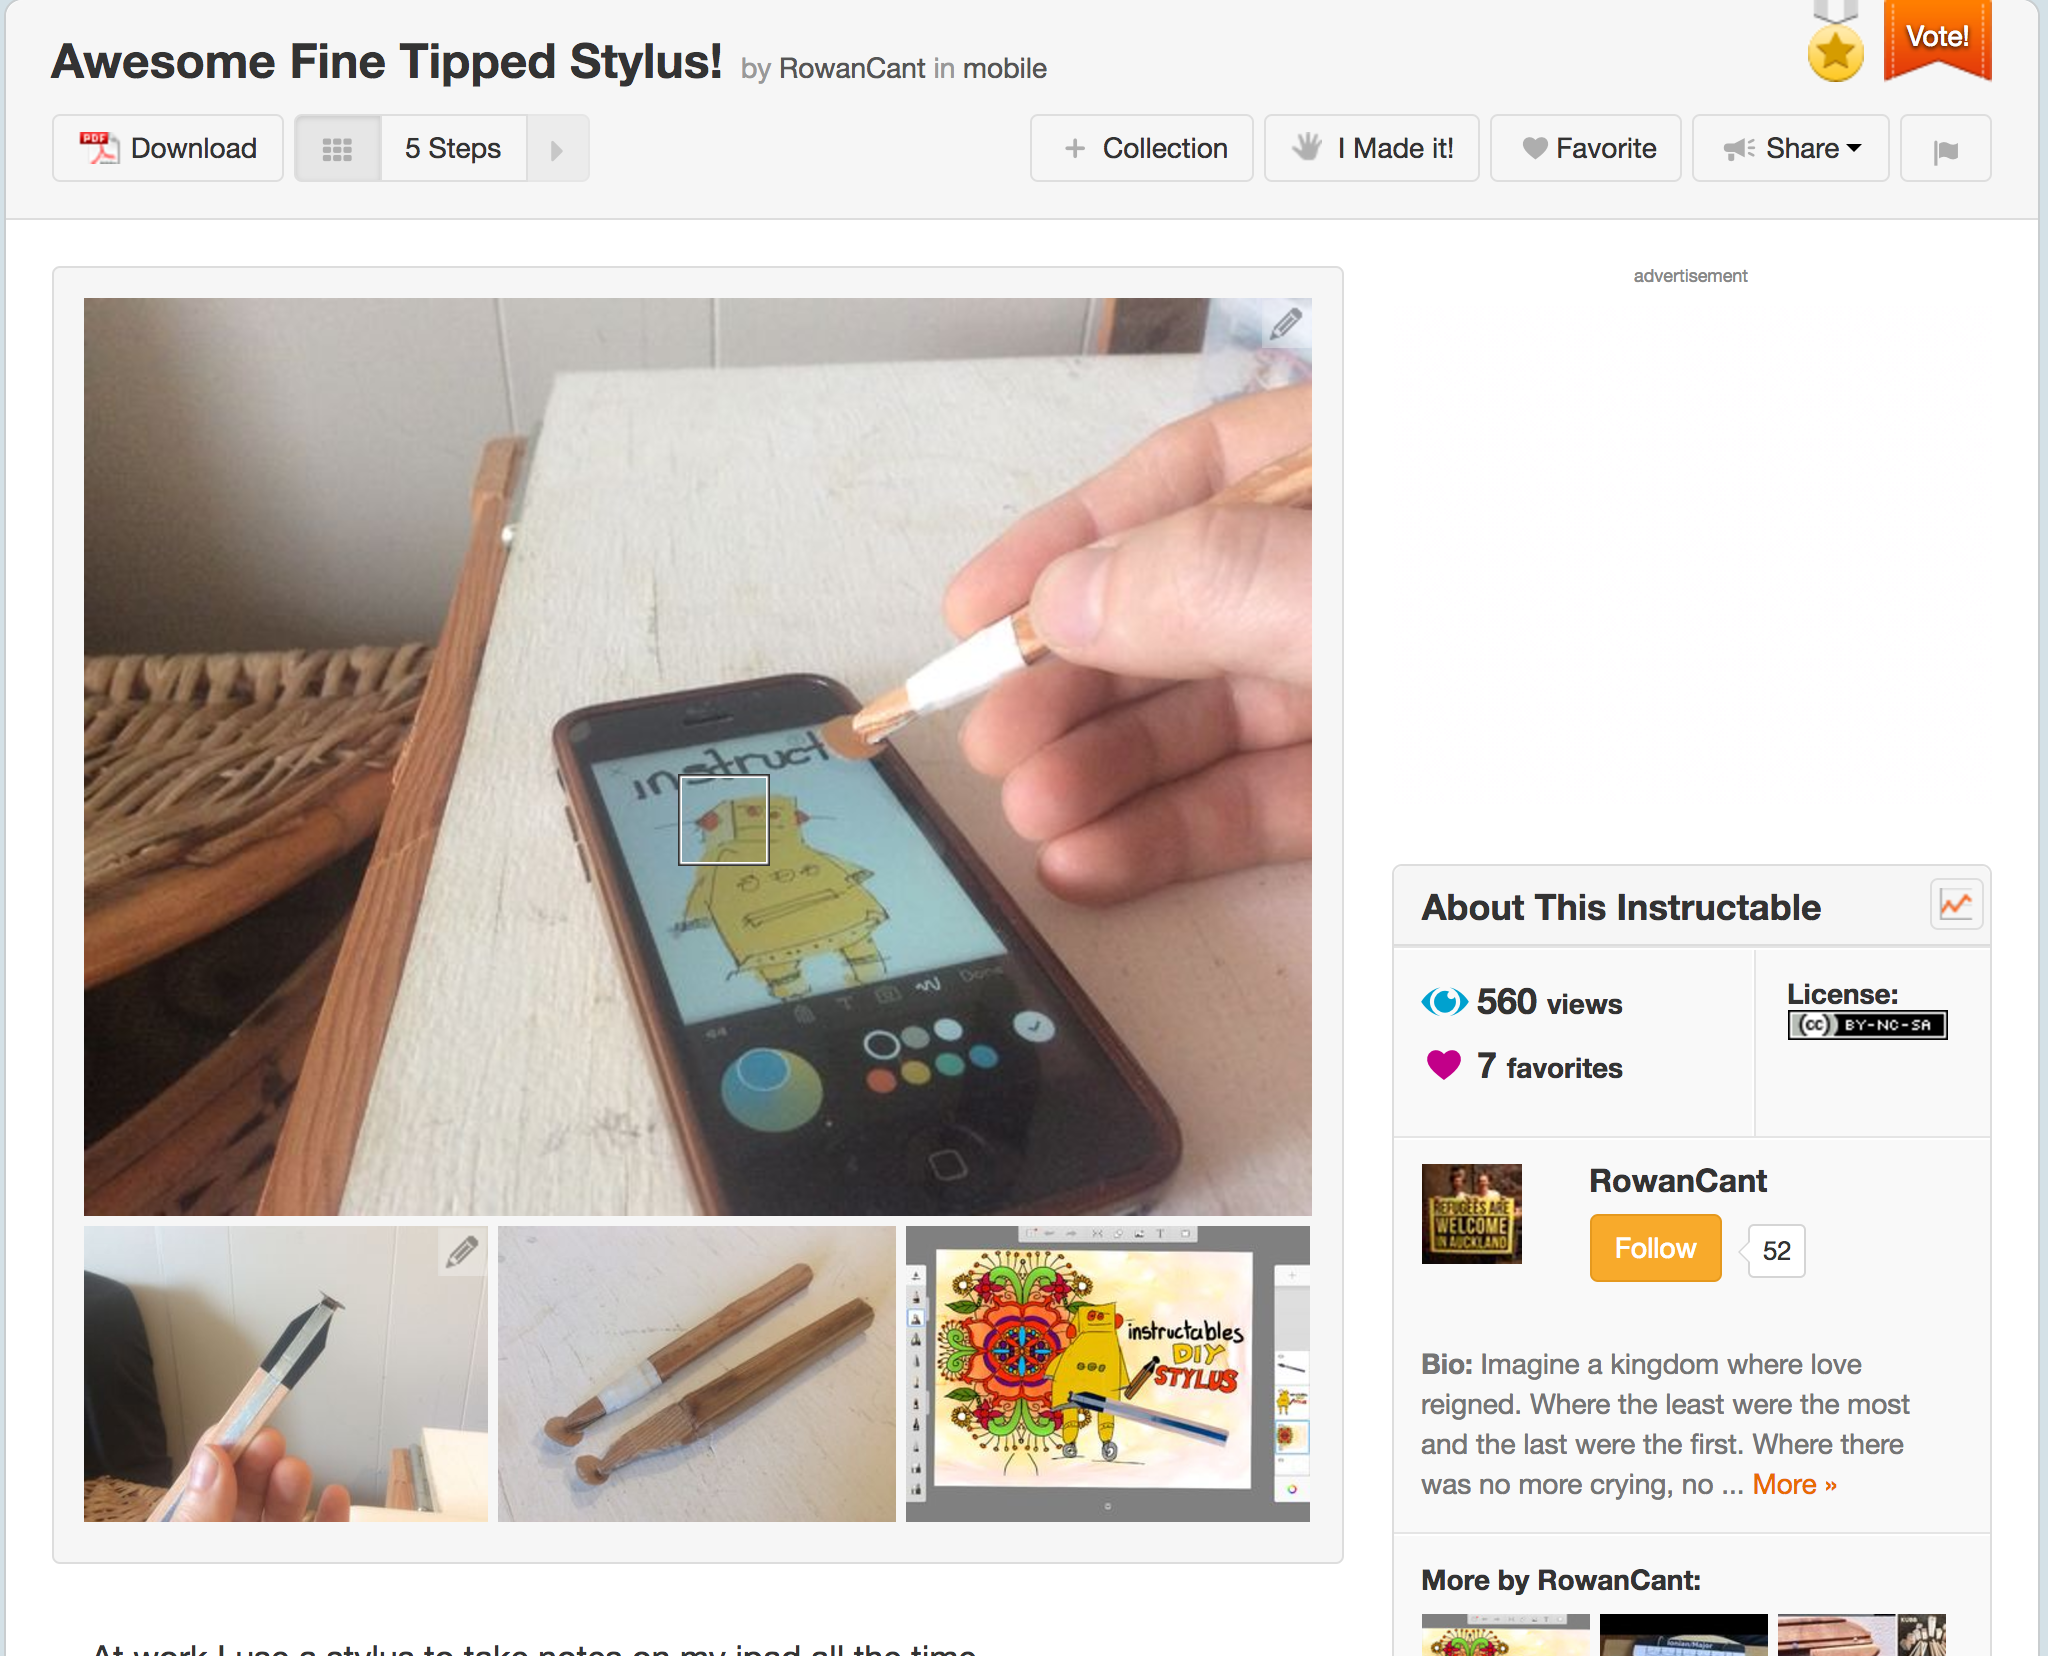
\includegraphics[scale=0.36]{./images/img-instructables.png}
	\caption{Sample Instructables project, \url{http://www.instructables.com/id/Awesome-Fine-Tipped-Stylus/}}
	\label{sec:img-instructables}
\end{figure}

Instructables is an online platform for \textit{DIY} communities that serves as a "place that lets you explore, document, and share your creations" \cite{web:instructable}. It is a website specializing in user-created and uploaded do-it-yourself projects, which other users can comment on and rate for quality \cite{wiki:instructable} \cite{wiki:instructable}. There are different categories of project such as technology, crafts, food, home, workshops and living, with more than 263,258 projects and 9,888,442 monthly visit as of August 2017. Users create their project step by step and with each step they describe what they did in a text, photos or videos as displayed in the figure \ref{sec:img-instructables}. The encapsulation of steps produce a typical guide that help others to re-create the project, learn from it or build a new thing on top of it and have their own version of the project. 

The contributions in Instructables come from the sharing culture of projects, not only authors contribute but also readers who can view and give feedback by commenting on the project. Also, Instructables create a social community where they exchange their thoughts about a topic via forums and subforms dedicated to a special topic such as Arduino projects. Finally, prizes are given to the top shared Instructables as a kind of reward for their effort of sharing their project and to keep them connected with the community.

\subsection{Methodology} 

To understand the users interactions of Instructables, an extensive study of the Instructables community has been done in the fall of 2011, this study used semi-structured interviews and online surveys. The semi-structured interviews had a framework of four themes that had been explored : (\oldstylenums{1}) motivation, (\oldstylenums{2}) Documentation tools, (\oldstylenums{3}) Writing an Instructable and (\oldstylenums{4}) Feedback. A theme was covered by a set of questions that took one hour with each interviewer. \cite{scholar:Tseng:2014:PVP:2598510.2598540}. A survey of 15 multiple-choice questions and open ended-questions that ask users about different aspects of their experience with replicating or building on top of a project shared by a user on the platform.

\subsection{User interaction}

The study has shown three strategies for documenting a project. The first was to \textit{write after you make}, as shown in the figure \ref{img-writemake}  \cite{tseng2016making}.
\begin{figure}[ht!]
	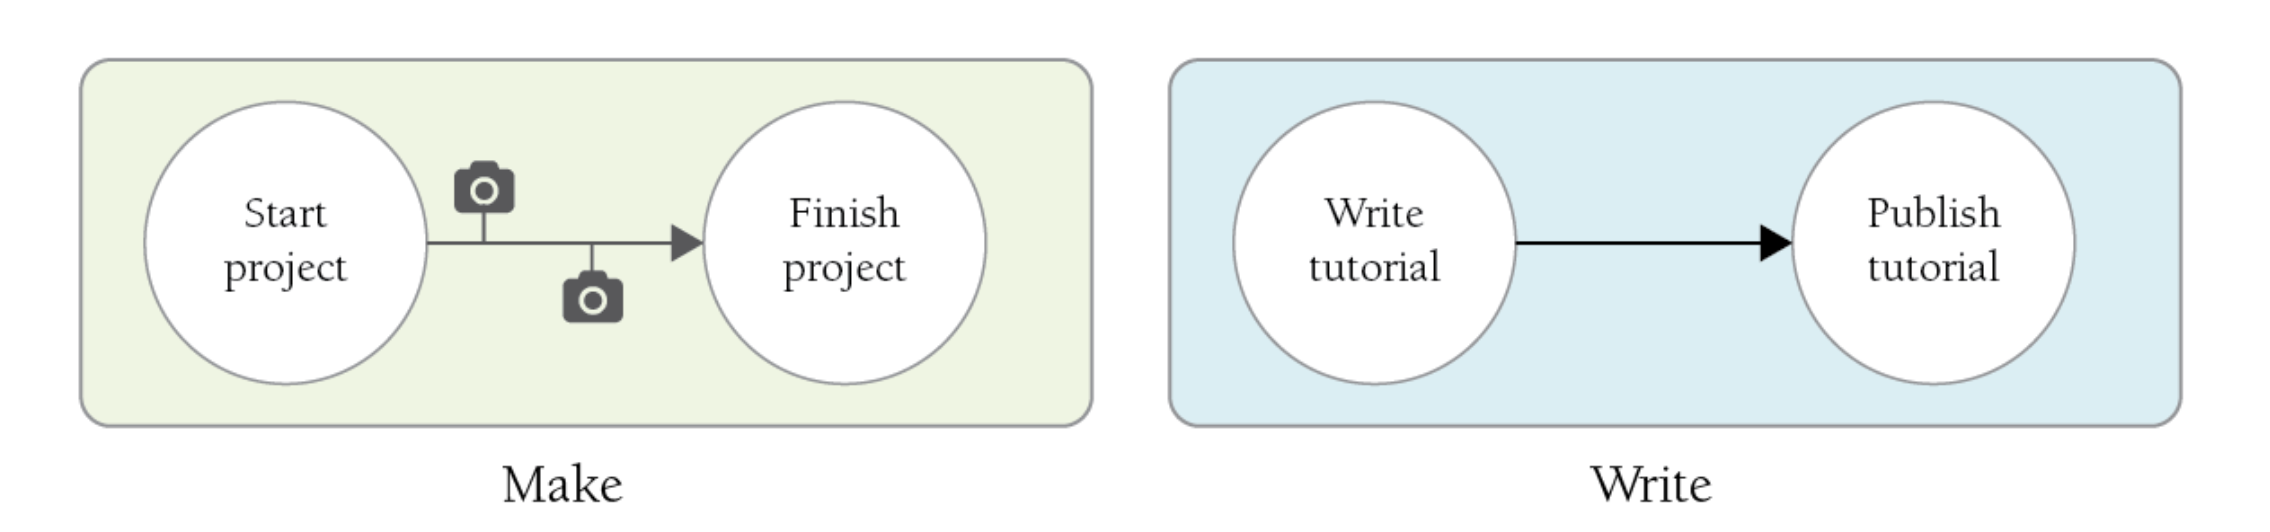
\includegraphics[scale=0.34]{./images/img-writemake.png}
	\caption{First strategy of documenting : write after you make, \cite{tseng2016making}}
	\label{img-writemake}
\end{figure}

A problem confronted the users with this strategy, users forgot to document in the midst of making. Users outperformed this problem by following the second strategy of \textit{writing after replicating}, as displayed in the figure \ref{img-makereplicatewrite} \cite{scholar:Tseng:2014:PVP:2598510.2598540}
\begin{figure}[ht!]
	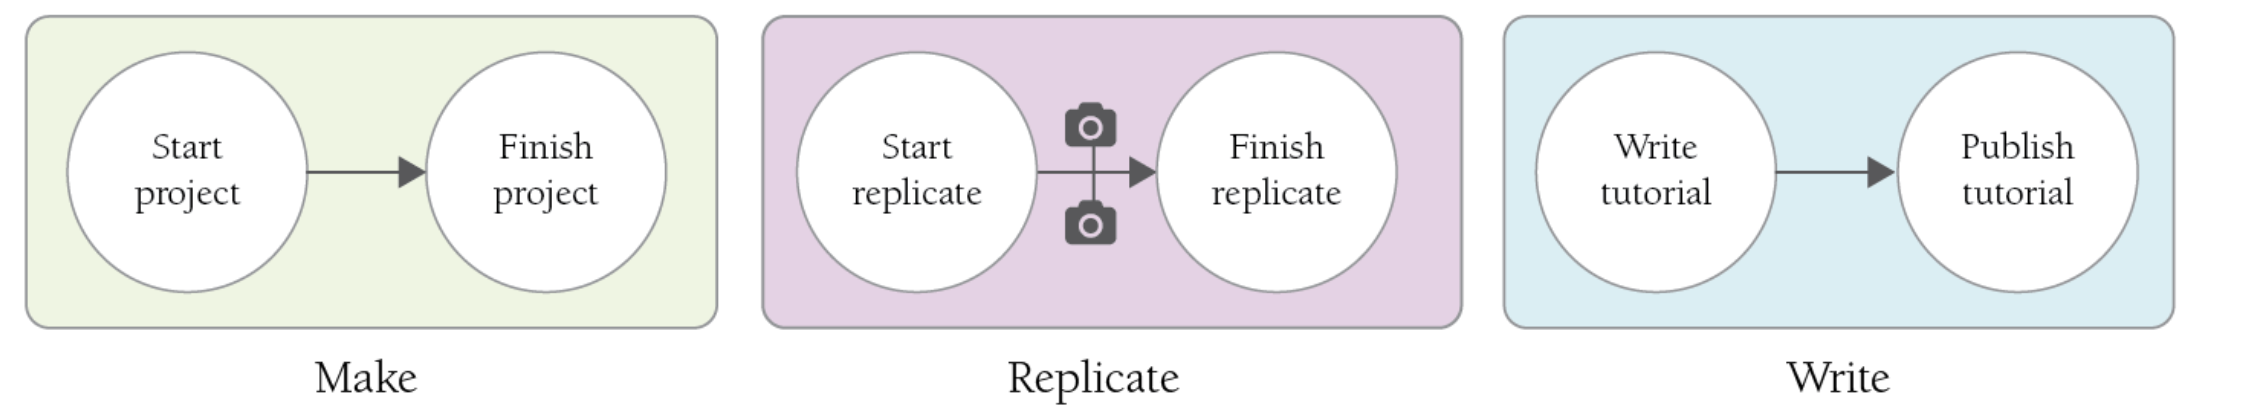
\includegraphics[scale=0.34]{./images/img-makereplicatewrite.png}
	\caption{First strategy of documenting : Make, replicate  then write, \cite{tseng2016making}}
	\label{img-makereplicatewrite}
\end{figure}

The final strategy was to \textit{simultaneously write and make} (figure \ref{img-makewritesimultanously}). 
\begin{figure}[ht!]
	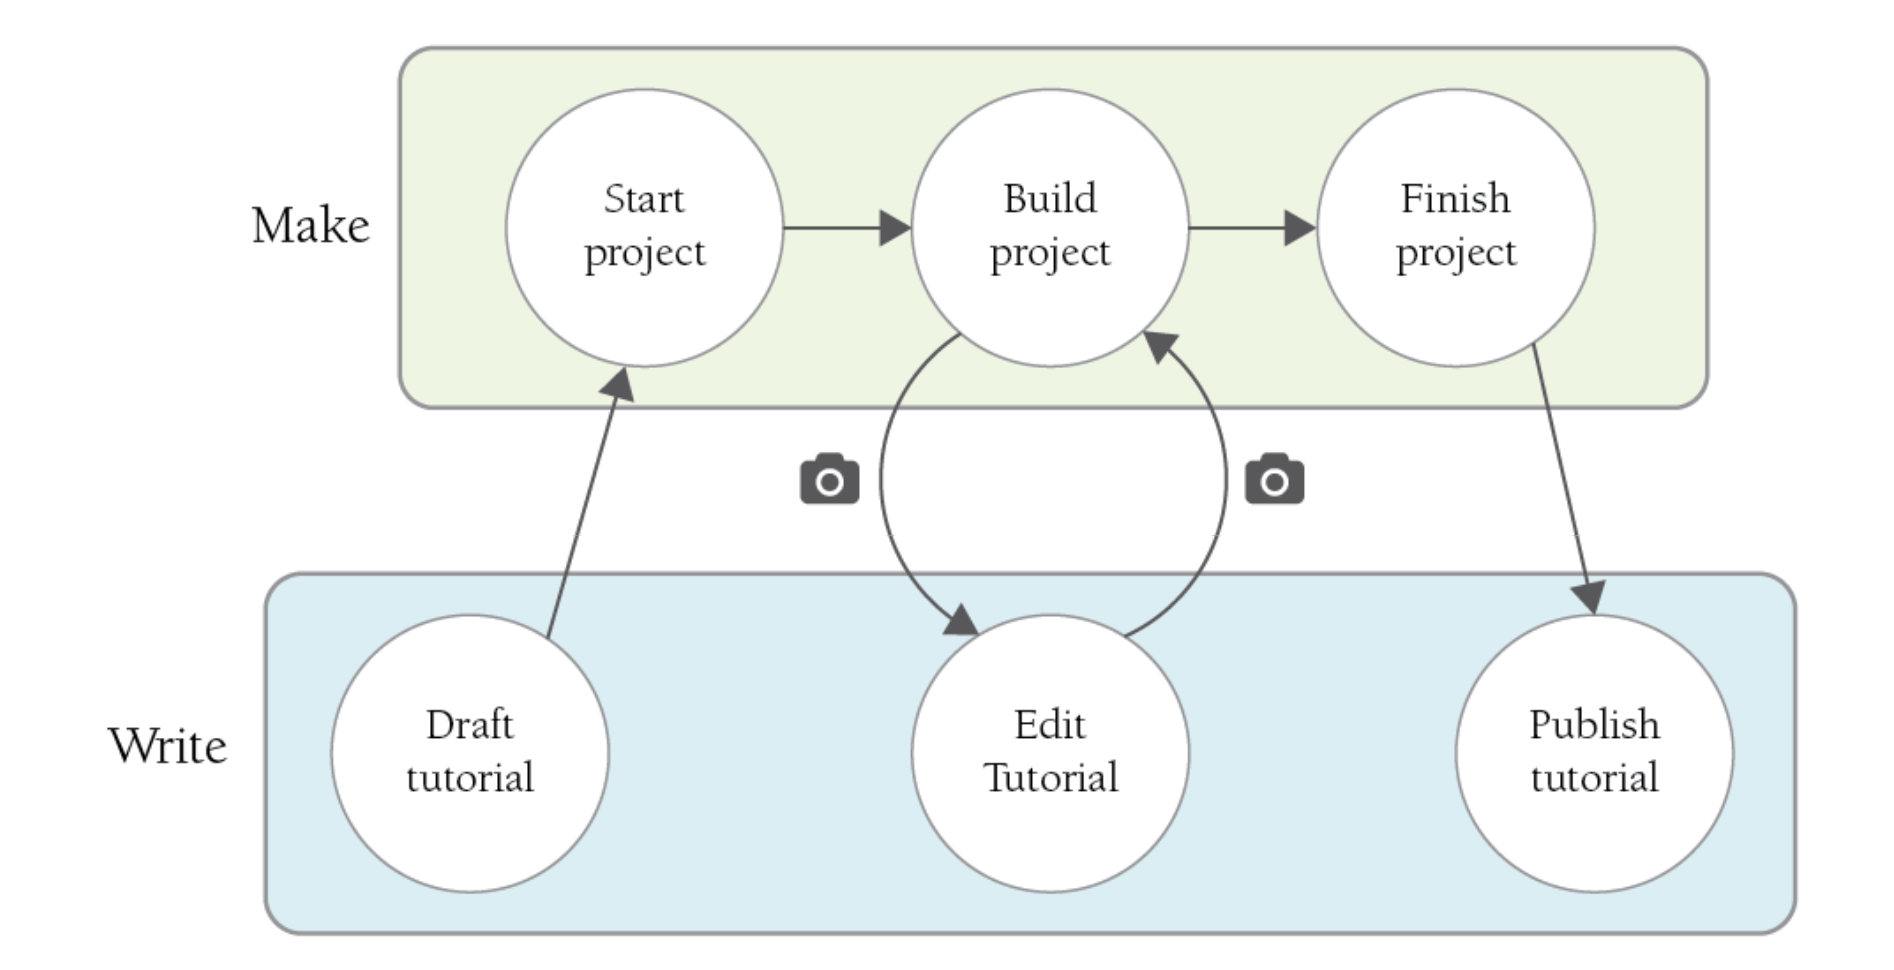
\includegraphics[scale=0.34]{./images/img-makewritesimultanously}
	\caption{First strategy of documenting : write after you make, \cite{tseng2016making}}
	\label{img-makewritesimultanously}
\end{figure}

In summary, the study showed that users need to encapsulate the collected photos and videos to show to create all the steps and a common challenge was to remember to document after each step otherwise users had to replicate their project merely to creating good documentation. 

Finally, authors saw that documentation well worth the effort to share their work but it is time consuming process when a project get more complex, it is hard to follow up or complete the documentation. \cite{scholar:Wakkary:2015:TAH:2702123.2702550}

\subsection{Design and process oriented documentation}
Several approaches were suggested by to improve the online documentation. Documentation techniques requires authors to simultaneously switch between making and writing, make a design process to not miss a step from not being documented or to radically recreate the project to document it in a proper way. Another challenges of documentation technique that needed to support not only the capture of digital artifacts but also physical artifacts where it is not possible to show the physical effort. 
With the recurring need to balance manual and automated ways of capturing, software and hardware tools need to solve open questions and be customizable for different activities and different audiences \cite{Kuznetsov:2010:REA:1868914.1868950}. The workflow of documentation over time needed to not miss a key step in the documentation. 

Documentation process seems to be more important for readers as it give them the opportunity to enable better decision making about components or materials to use \cite{scholar:sf1241364}, as well as successful in encouraging independent exploration and fostering a sense of accomplishment \cite{scholar:lovell2010sewing}. Also, as many users start by replicating some projects, having tools where they could be able to contribute to a project, can help more socializing and boost a collaborative work in the community. 

\section{Build In Progress}
%\hl{What is it ?} \hl{Who use it ?} \hl{User interactions ?} \hl{Limitations} \hl{Advantages ?} \hl{Examples ?}

Build in Progress is a platform for sharing the story of your design process, where \textit{"makers share how their DIY projects evolve over time}" \cite{tseng2016making}. It focus more on the storytelling of \textit{DIY} documented project, a snapshot of the platform displayed in the figure \ref{img-buildinprogress}.

BiP was launched in 2013 and within a collaboration with many institutions and a network of schools, it hosted over 1368 projects in categories such as Electronics, Mechanical and living. Users contributed to BiP community by sharing, providing feedback and describing their progress of each step, the encapsulation of informations lead to a story about the project as BiP "\textit{support a storytelling approach to documentation}" \cite{tseng2016making}.
\begin{figure}[ht!]
	\centering
	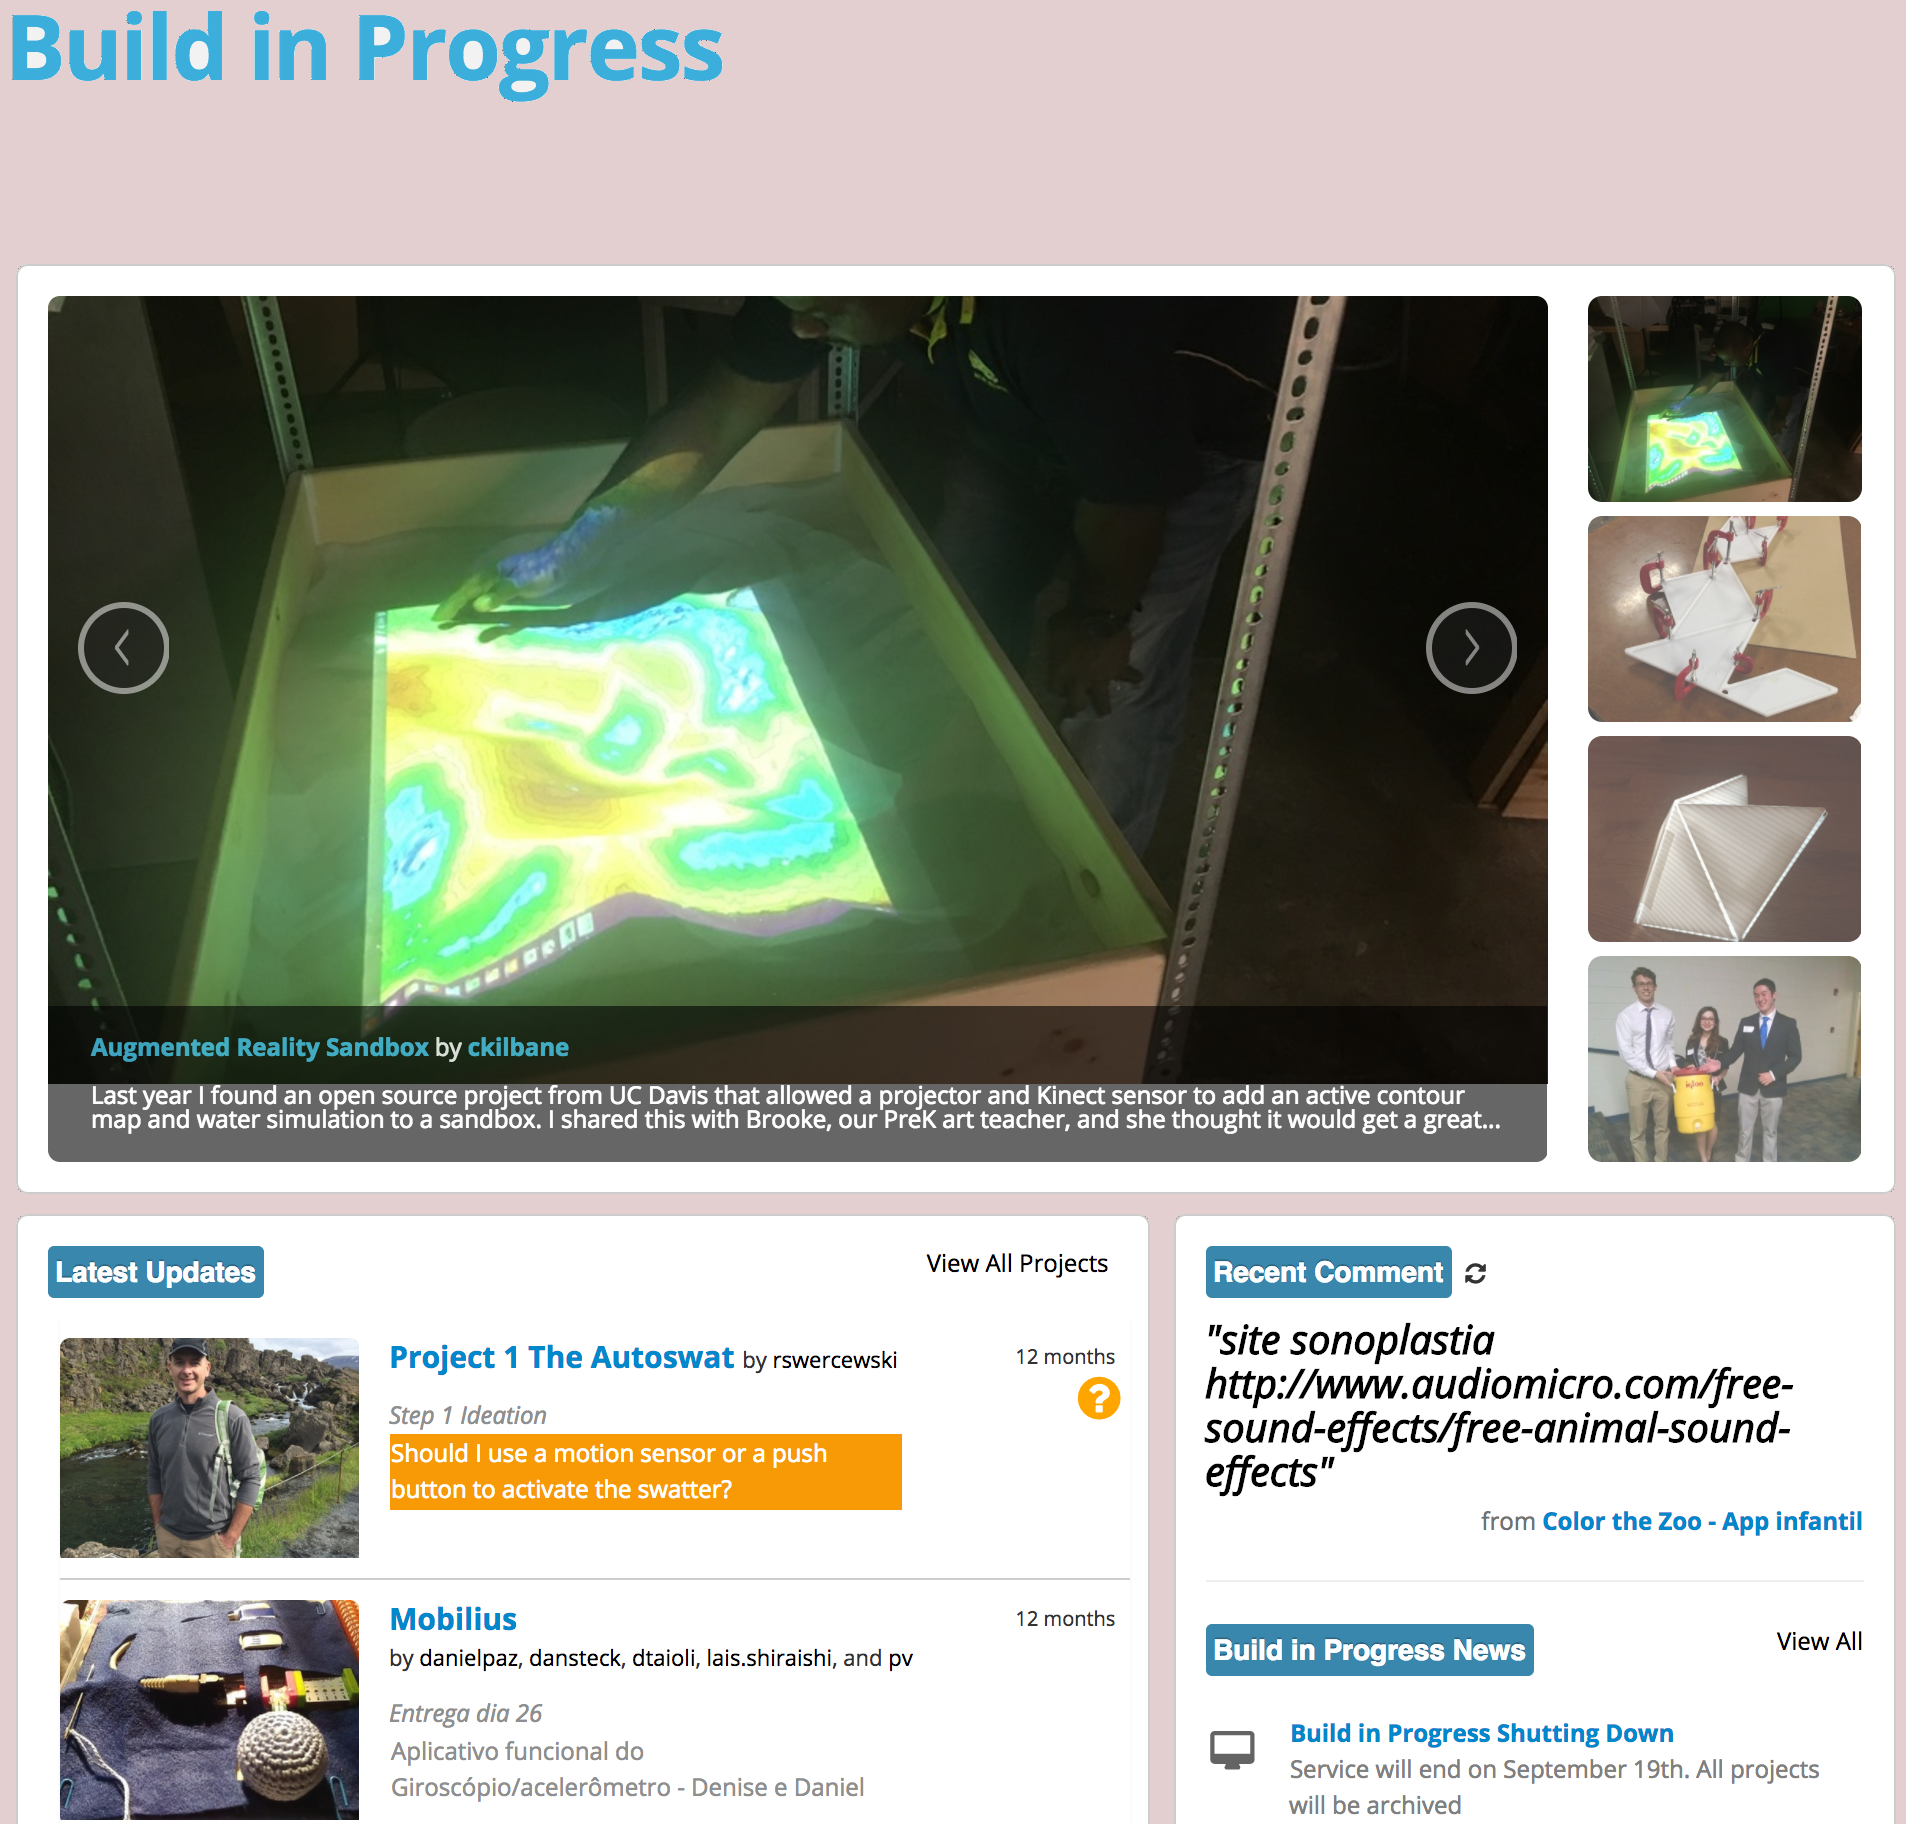
\includegraphics[width=10cm, height=10cm]{./images/img-buildinprogress.png}
	\caption{Build in progress welcome page, \cite{BuildinP1}} 
	\label{img-buildinprogress}
\end{figure}

\vspace{-1cm}
\subsection{Design approach}
Authors shared an iterative design process in the context of sharing their personal journey by creating step-by-step instructions of their project via the online platform \textit{BiP} and companion mobile application. Readers contributed by suggesting to makers after publishing their steps, makers benefited from sharing step-by-step instructions over time by taking into account the suggestions of readers.

BiP was developed based on an innovative design process, it enables users to visualize their documentation in an iterative way. Authors can continuously iterate their building process, share their techniques to help others to reach out others in the community so they can have feedback. A social design process principle was considered among the online community to engage users more, to accumulate knowledge, to learn from others and connect users with same interest as \textit{human-related issues in the form of social ties and knowledge sharing were reported as keys to successful collaboration} \cite{Kotlarsky2005}.

\subsection{Features}\label{sec:feature}
BiP consists of many features in the project page and social feature. The two core features of the project page are : the \textit{Process Map} and \textit{Step Detail View } (\ref{img-bipprojectpage}).
\begin{figure}[ht!]
	\centering
	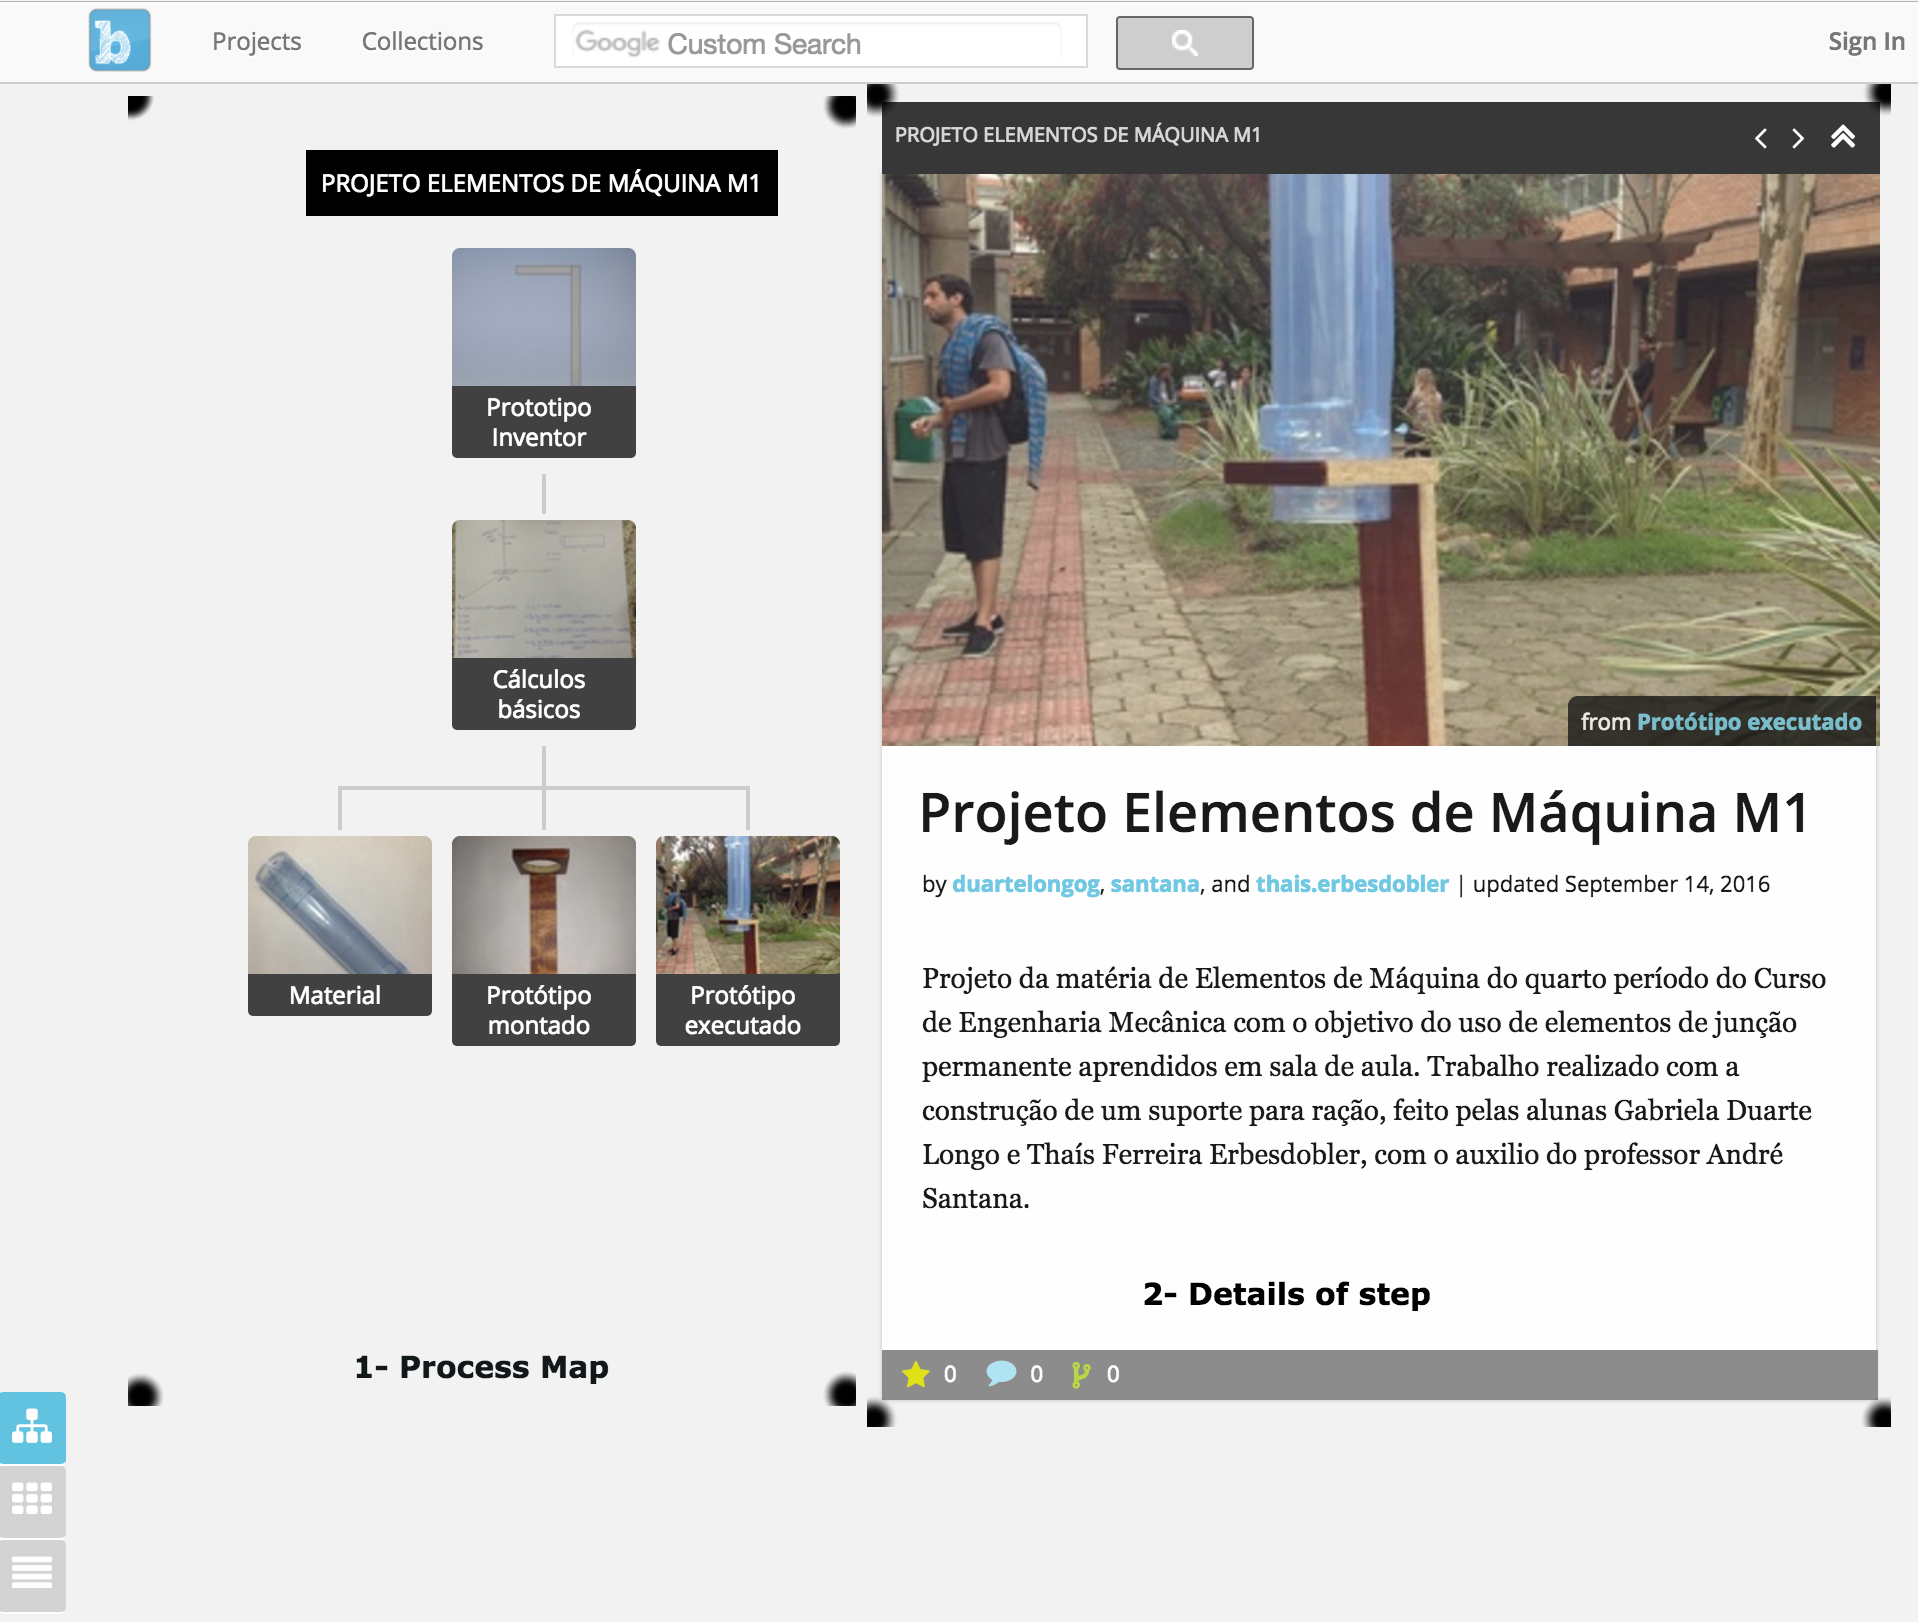
\includegraphics[width=.3\textheight]{./images/img-bipprojectpage.png}
	\caption{overall project view, \cite[\url{http://buildinprogress.media.mit.edu/projects/4599/steps}]{BuildinP1}} 
	\label{img-bipprojectpage}
\end{figure}
In the process map, users can create a step, a label for one or more step, drag \& drop  to rearrange steps. Steps are organized in a tree-map-like format with sui generis branches, a label is added to a branch and it can be colored to designate a branch; for example orange labels represent that a branch is in progress.

Project are displayed in 3 different mode.  The first is the default mode : tree-map, users can go through all the steps, step-by-step and discover more about it as shown in figure \ref{img-mode1}.
\begin{figure}[H]
	\centering
	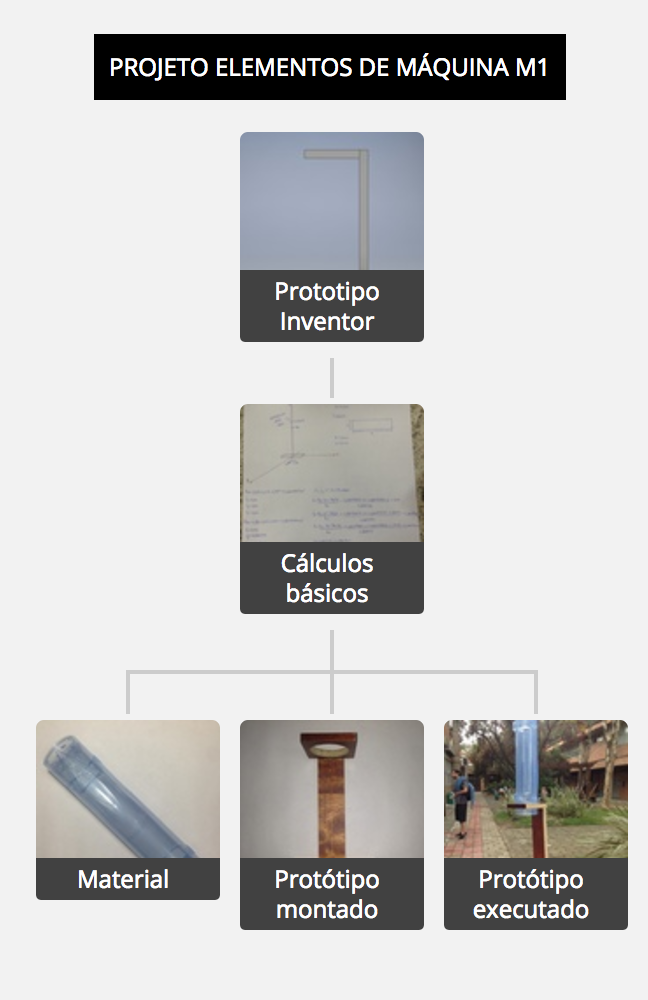
\includegraphics[scale=.3]{./images/img-mode1.png}
	\caption{tree-map view of the project} 
	\label{img-mode1}
\end{figure}

The second is Gallery mode \ref{img-mode2} and finally  the  blog mode : users can scroll down and an index of steps will be displayed on their left side of the page (figure \ref{img-mode3}).

\begin{figure}[H]
	\centering
	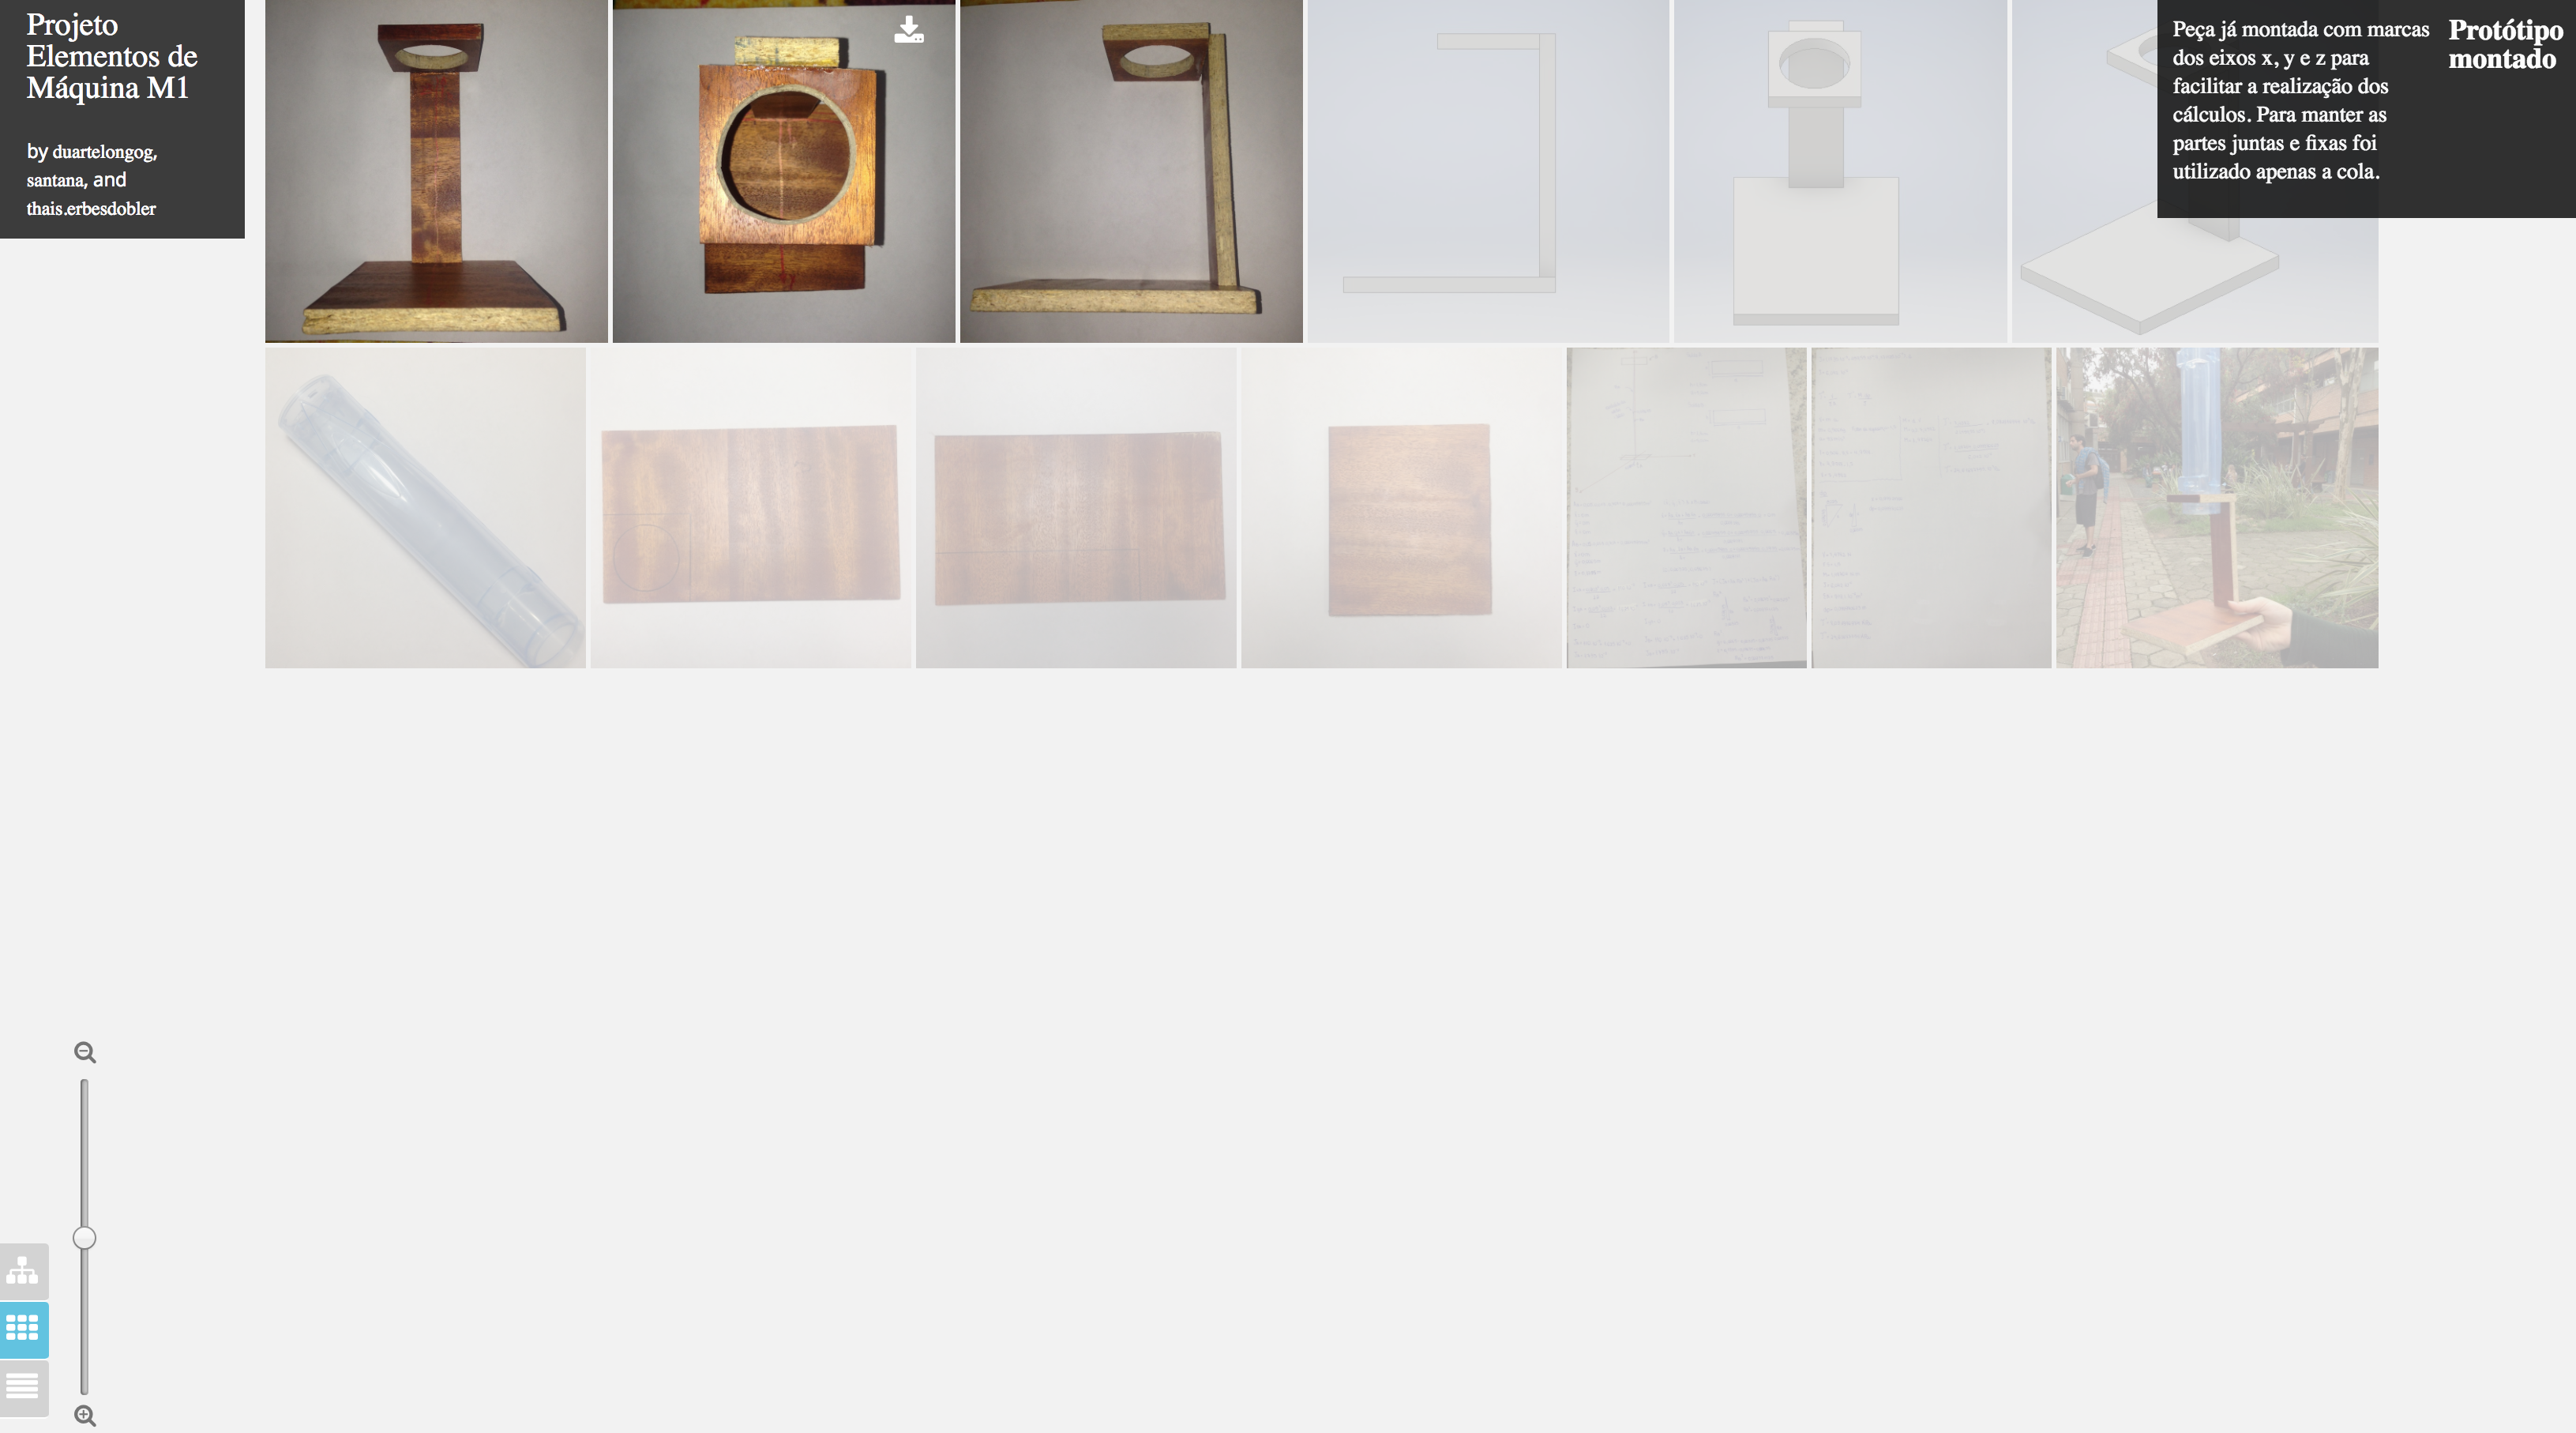
\includegraphics[scale=.16]{./images/img-mode2.png}
	\caption{Gallery view of the project} 
	\label{img-mode2}
\end{figure}

\begin{figure}[H]
	\centering
	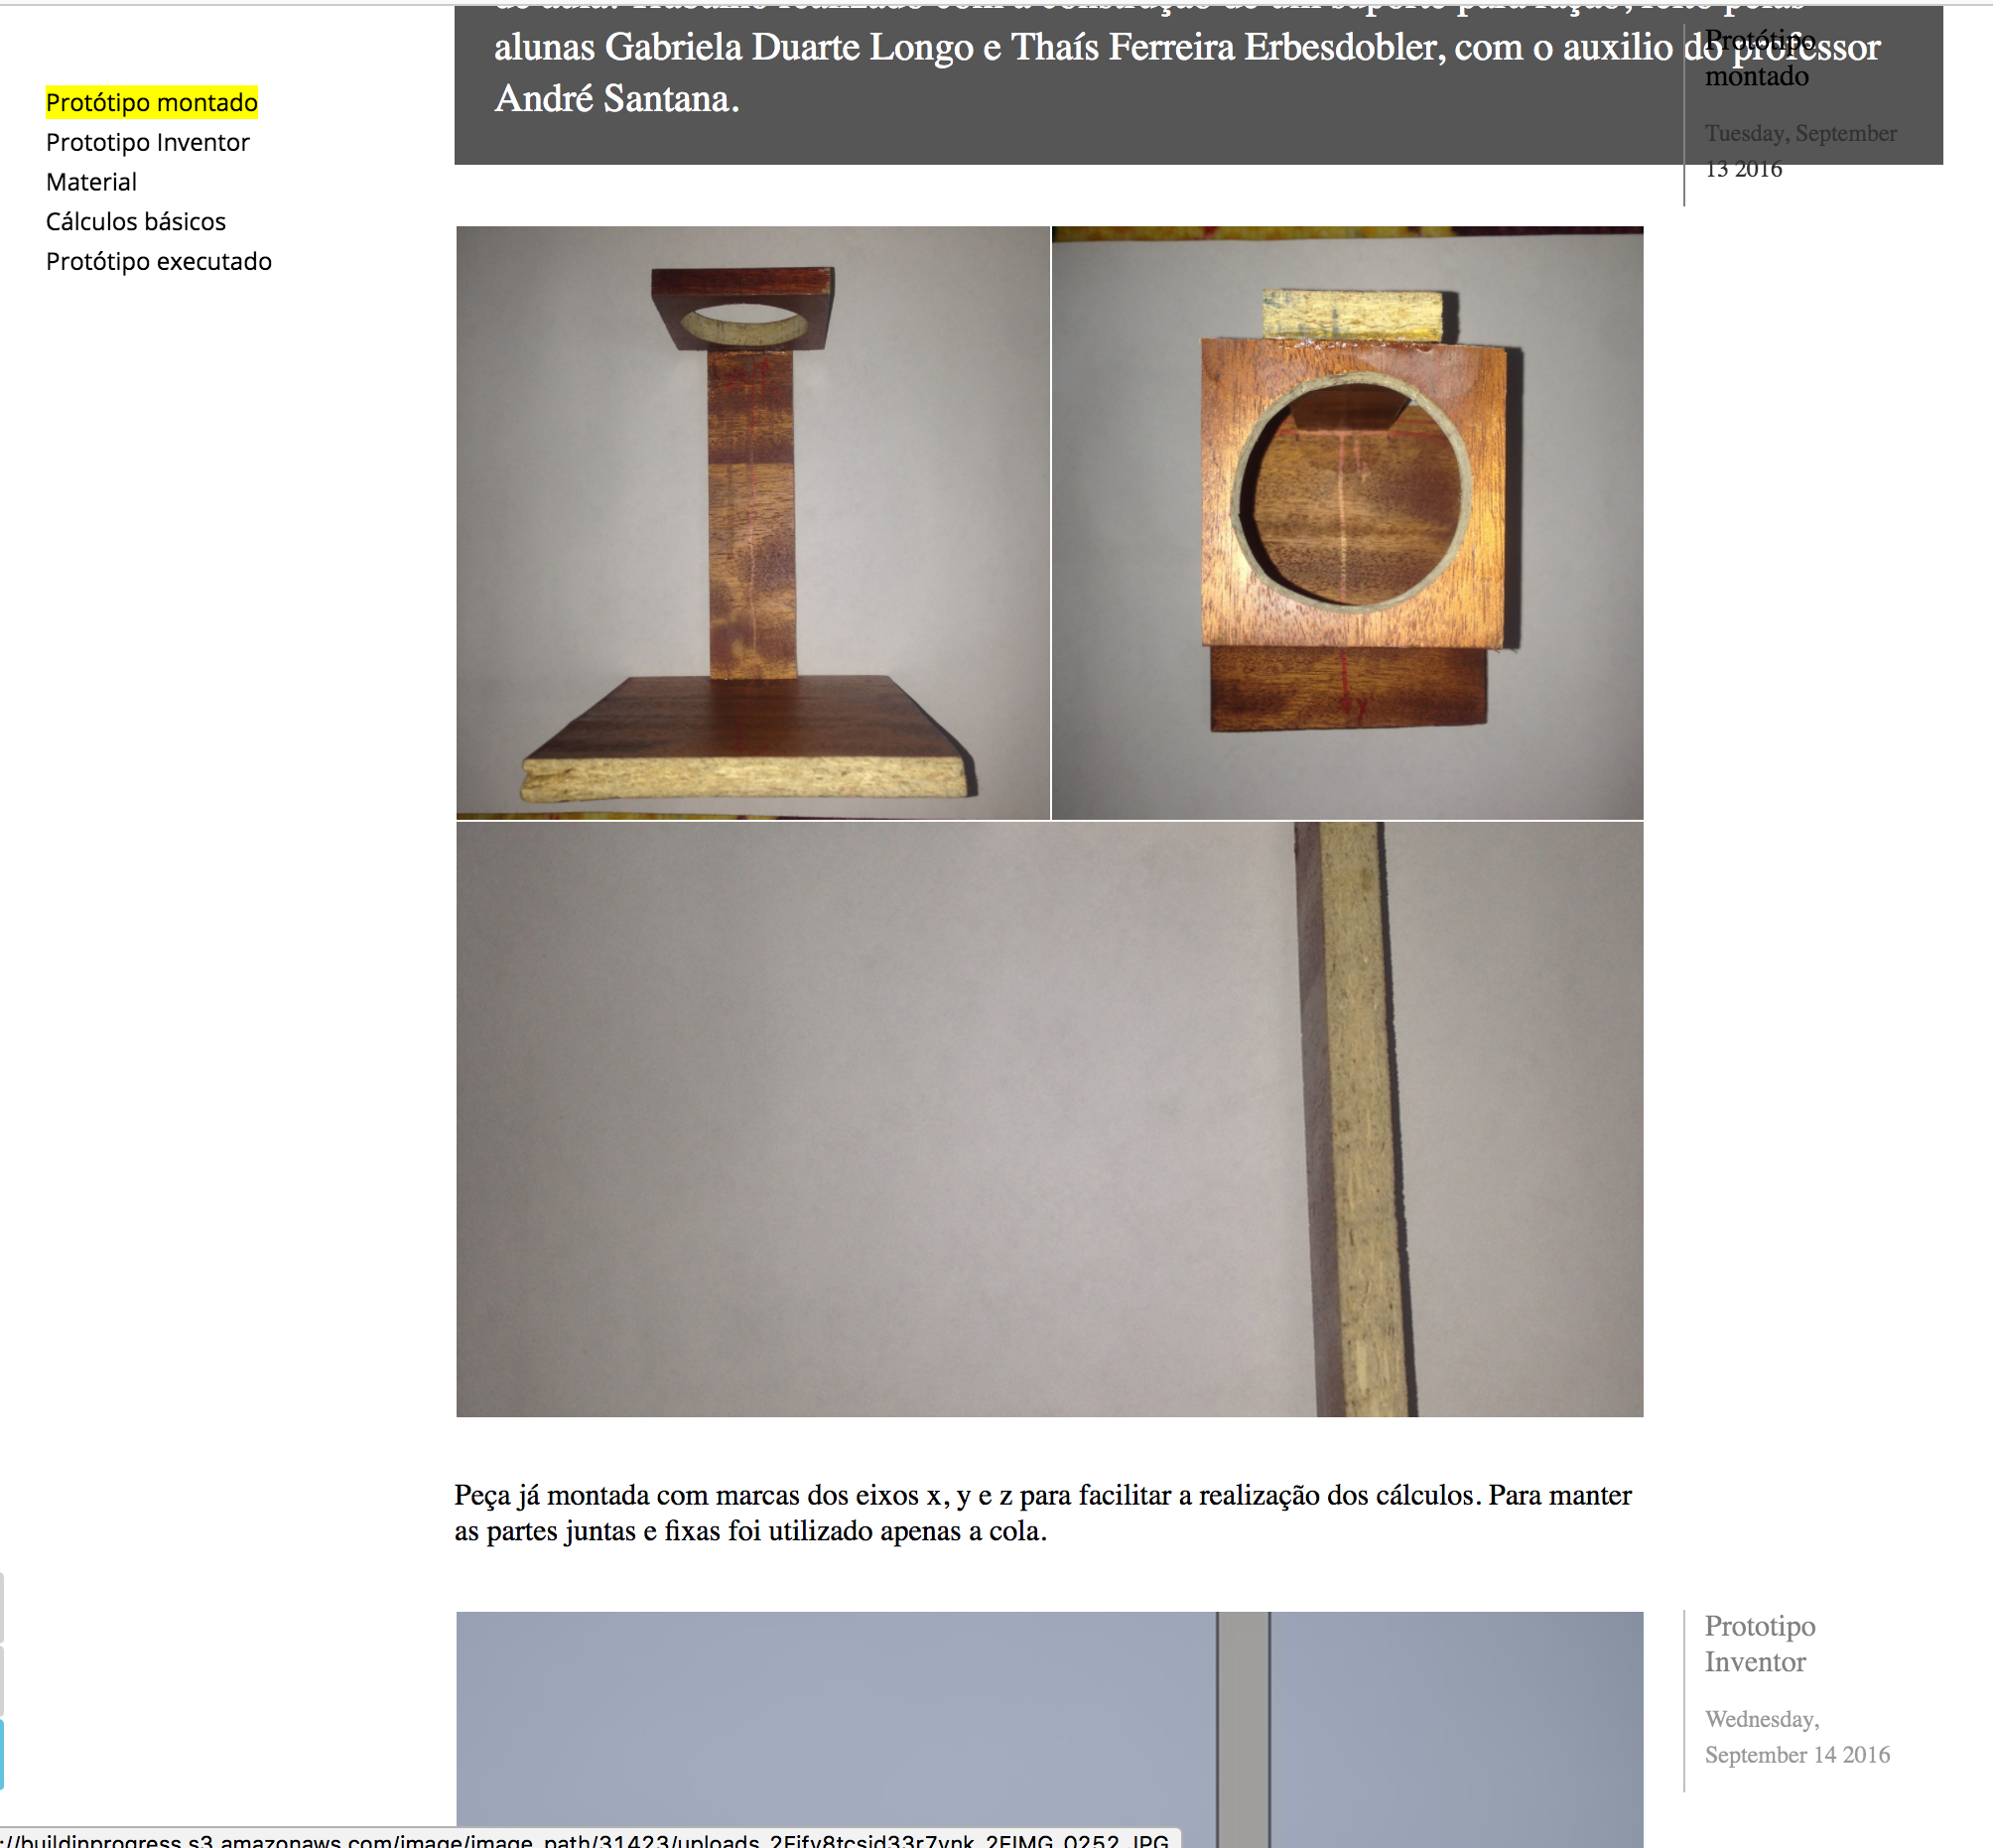
\includegraphics[scale=.3]{./images/img-mode3.png}
	\caption{Blog like mode} 
	\label{img-mode3}
\end{figure}

In \textit{Details of step} users can upload photos or videos, add text description, ask others a question that will appear in the homepage of the platform, upload resources or files in different formats; e.g. .PDF, .PPT, a given example is shown in the figure \ref{img-stepdetails} .
\begin{figure}[H]
	\centering
	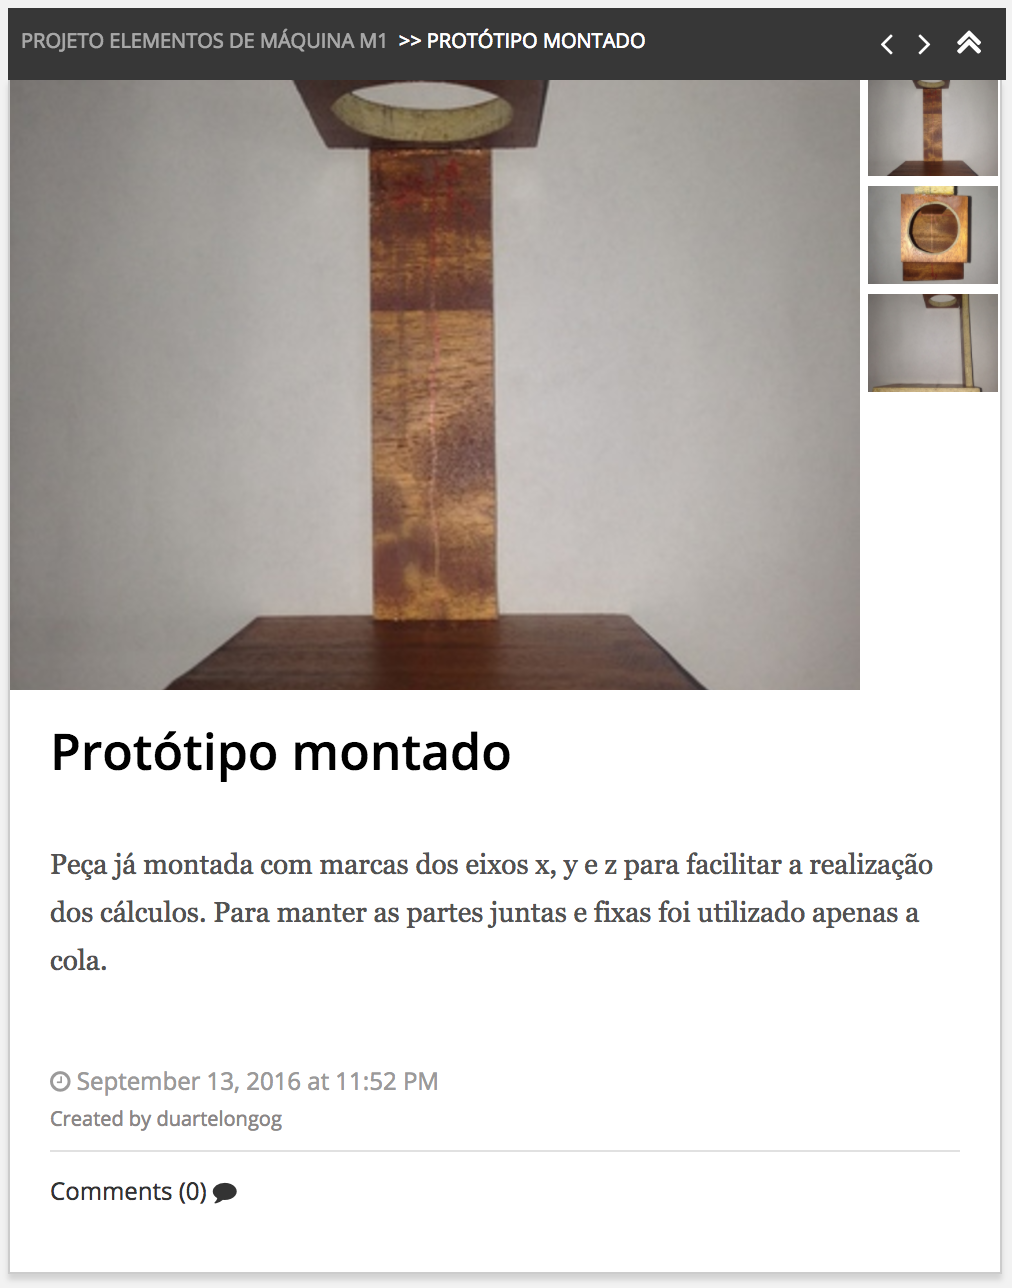
\includegraphics[scale=.3]{./images/img-stepdetails.png}
	\caption{Details steps view} 
	\label{img-stepdetails}
\end{figure}

The online platform incorporate many features that keep the BiP community more socialized and connected. Users can follow a project, see recent activity on the homepage and they will receive notification once an author add a step or ask a question.
\begin{figure}[H]
	\centering
	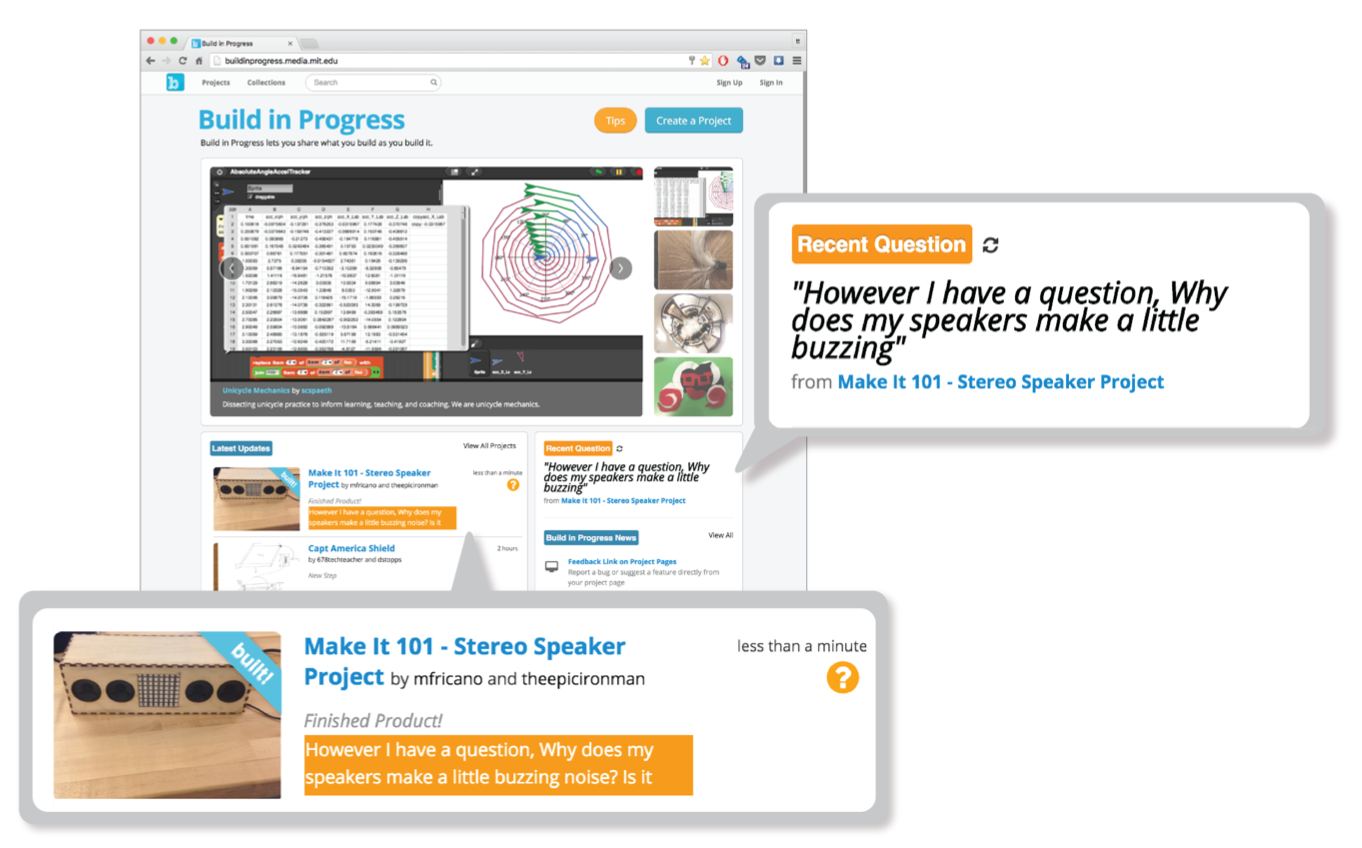
\includegraphics[scale=.4]{./images/img-commentquestion.png}
	\caption{Question featured in the home page, [Tseng, 2016]} 
	\label{img-commentquestion}
\end{figure}

Moreover, users can leave a text on any step and they will receive a notification when a comment is left. Authors can ask for feedback or help by embedding a question that will be added to the Community Activity section of the homepage, see figure \ref{img-commentquestion}.
\subsubsection{Mobile application}
A mobile application has been created to make documentation more efficient in which users upload images and videos to their projects directly from their devices instead of taking picture from their devices then transfer it to a computer and upload it (figure \ref{img-mobileapp}.
\begin{figure}[H]
	\centering
	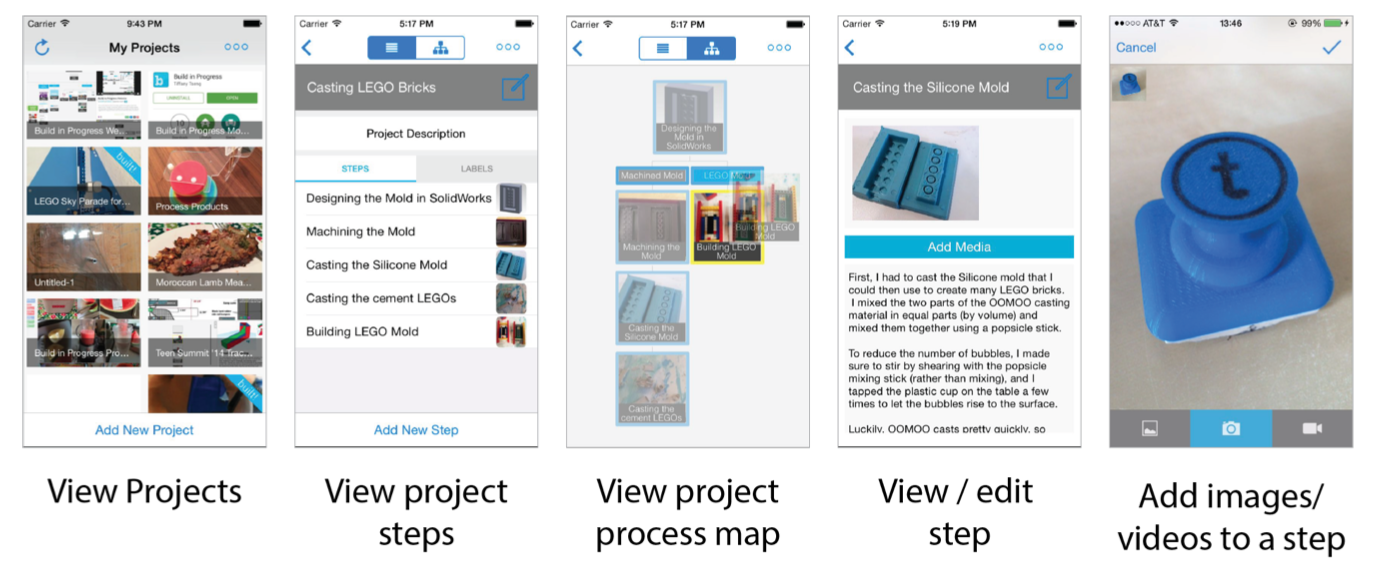
\includegraphics[scale=.5]{./images/img-mobileapp.png}
	\caption{Mobile application interface, [Tseng, 2016]} 
	\label{img-mobileapp}
\end{figure}
\subsection{User interaction}

BiP has been used in after-school  programs, in school and in workshop challenges by students and makers who work on their own project. Teenagers and one adult facilitator have been interviewed and a weekly survey was sent to all users to get an estimation about their weekly hours work.

The results of the interviews and surveys showed that users get motivated to share their project as it facilitate getting feedback, create and show their portfolio projects, get engaged to document and to help others. Users found that BiP support meaningful documentation practices and many strategies were identified depending on the type of project, the duration of a project and the age of makers who are using it.

\subsection{Summary}

The study of BuildinProgress showed that BiP support authors and readers. The documentation help makers to create a design process for their project by learning from the many iterations they did over time and BiP motivates reflective practice on making, design process, and values and identity. Users get engaged, get feedback, get self reward and help others. It support all capturing way written and visual. 



\section{Discussion}

\textit{BuildinProgress} and \textit{Instructables} didn't bring a new fundamental way in which users can share their captured media publicly or in private. Design parameters can be adjusted to support different type of users-interactions and goals.  Instructables enable users to personalize through substitution and modification of a step and any missing step mean that authors should re-create their documentation while BiP focus more on the  design process where users can iterate their project by creating new branches and forget about the unsuccessful branches.

The mix between capturing and text-based-description features in BiP enable teenagers to document. The ease of use for creating a branch, drag \& drop simplify the job for younger audience especially readers who are new to the community of \textit{DIY} as they can go through steps, iterate on their work, modify a step or re-arrange some steps.  Instructables has both features but there is no friendly structure where authors get their documentation organized and if an author has a limited background in documentation or he doesn't like it, he will probably abandon the documentation of a project after the first type a user find that it is not possible to re-arrage the documented steps.

Sharing a project is not enough for authors. Users in Instructables found that they cannot share their thought or it is limited as the only way to express what they think is via a comment. BiP offers a text-based option where both authors and readers could ask a question or leave a comment, also, both can receive a notifications for a reply from the community or any other news concerning any modification in the project.

The process of sharing the effort in progress enable users to communicate more in BiP, they helped each other, they showed their effort, they get featured and receive feedback as described in section \ref{sec:feature}. Balancing the ease of use of automated documentation systems with the powerful feature, a mobile application, encourage more users to upload pictures or videos and enable them to be physically free so they can move around to document their project for example without having the problem of taking a photo, remember which step it is, transfer it then upload it to the platform as in Instructables.

\begin{comment}

\begin{itemize}
	\item{Adapt  SDG in progress}
	
	
	\item{Qu-est ce que la platforme a apporte et ce que nous on a apporte}
	\item{Comparaison avec other platform}
	\item{ Explication about the summer school, experience, different way to document etc..} 
	\item{When we can use it and how we can use it ?} 
	
\end{itemize}


\begin{itemize}
	\item Platforme pour le soutien des hackathon grise
	\item What tiffanz said about here ieda and references
	\item securite constructif
	
	\begin{itemize}
		\item la continuite des  idess
		\item durabilitz of projects
		\item relance les projet
	\end{itemize}
	\item hackathons
	\item summer school
	\item master
	\item how to evaluate a project in time when it avaluate from team to team
	\item changement de step ou de team, continuite sachant qu'on connait des interruption forte , d'etape, d'equipe, et les 2 rests ensemble
	\item cumulative innovation
	\item in innnovation find a waz to document goodlz 
	\item rice made
	\item 
\end{itemize}

\section{IDEAS}
\begin{itemize}
	\item "Users don't want documentation, they want answers" 
\end{itemize}

\section{Features}

%% This is an example first chapter.  You should put chapter/appendix that you
%% write into a separate file, and add a line \include{yourfilename} to
%% main.tex, where `yourfilename.tex' is the name of the chapter/appendix file.
%% You can process specific files by typing their names in at the 
%% \files=
%% prompt when you run the file main.tex through LaTeX.




\label{sec:features}

The rest of this document shows off a few features of the template
files.  Look at the source code to see which macros we used!

The template is divided into \TeX{} files as follows:
\begin{enumerate}
\item \texttt{thesis.tex} is the main file.
\item \texttt{extrapackages.tex} holds extra package includes.
\item \texttt{layoutsetup.tex} defines the style used in this document.
\item \texttt{theoremsetup.tex} declares the theorem-like environments.
\item \texttt{macrosetup.tex} defines extra macros that you may find
useful.
\item \texttt{introduction.tex} contains this text.
\item \texttt{sections.tex} is a quick demo of each sectioning level
available.
\item \texttt{refs.bib} is an example bibliography file.  You can use
Bib\TeX{} to quote references.  For example, read
\cite{bringhurst1996ets} if you can get a hold of it.
\end{enumerate}


\subsection{Extra package includes}

The file \texttt{extrapackages.tex} lists some packages that usually
come in handy.  Simply have a look at the source code.  We have
added the following comments based on our experiences:
\begin{description}
\item[REC] This package is recommended.
\item[OPT] This package is optional.  It usually solves a specific
problem in a clever way.
\item[ADV] This package is for the advanced user, but solves a problem
frequent enough that we mention it. Consult the package's
documentation.
\end{description}

As a small example, here is a reference to the Section \emph{Features}
typeset with the recommended \package{varioref} package:
\begin{quote}
See Section~\vref{sec:features}.
\end{quote}


\subsection{Layout setup}

This defines the overall look of the document -- for example, it
changes the chapter and section heading appearance.  We consider this
a `do not touch' area.  Take a look at the excellent \emph{Memoir}
documentation before changing it.

In fact, take a look at the excellent \emph{Memoir} documentation,
full stop.


\subsection{Theorem setup}

This file defines a bunch of theorem-like environments.

\begin{theorem}
An example theorem.
\end{theorem}

\begin{proof}
Proof text goes here.
\end{proof}

Note that the q.e.d.\ symbol moves to the correct place automatically
if you end the proof with an \texttt{enumerate} or
\texttt{displaymath}.  You do not need to use \verb-\qedhere- as with
\package{amsthm}.

\begin{theorem}[Some Famous Guy]
Another example theorem.
\end{theorem}

\begin{proof}
This proof
\begin{enumerate}
\item ends in an enumerate.
\end{enumerate}
\end{proof}

\begin{proposition}
Note that all theorem-like environments are by default numbered on
the same counter.
\end{proposition}

\begin{proof}
This proof ends in a display like so:
\begin{displaymath}
f(x) = x^2.
\end{displaymath}
\end{proof}


\subsection{Macro setup}

For now the macro setup only shows how to define some basic macros,
and how to use a neat feature of the \package{mathtools} package:
\begin{displaymath}
\abs{a}, \quad \abs*{\frac{a}{b}}, \quad \abs[\big]{\frac{a}{b}}.
\end{displaymath}

This is version \verb-v1.4- of the template.

We assume that you found this template on our institute's website, so
we do not repeat everything stated there.  Consult the website again
for pointers to further reading about \LaTeX{}.  This chapter only
gives a brief overview of the files you are looking at.

\section{Features}
\label{sec:features}

The rest of this document shows off a few features of the template
files.  Look at the source code to see which macros we used!

The template is divided into \TeX{} files as follows:
\begin{enumerate}
\item \texttt{thesis.tex} is the main file.
\item \texttt{extrapackages.tex} holds extra package includes.
\item \texttt{layoutsetup.tex} defines the style used in this document.
\item \texttt{theoremsetup.tex} declares the theorem-like environments.
\item \texttt{macrosetup.tex} defines extra macros that you may find
useful.
\item \texttt{introduction.tex} contains this text.
\item \texttt{sections.tex} is a quick demo of each sectioning level
available.
\item \texttt{refs.bib} is an example bibliography file.  You can use
Bib\TeX{} to quote references.  For example, read
\cite{bringhurst1996ets} if you can get a hold of it.
\end{enumerate}


\subsection{Extra package includes}

The file \texttt{extrapackages.tex} lists some packages that usually
come in handy.  Simply have a look at the source code.  We have
added the following comments based on our experiences:
\begin{description}
\item[REC] This package is recommended.
\item[OPT] This package is optional.  It usually solves a specific
problem in a clever way.
\item[ADV] This package is for the advanced user, but solves a problem
frequent enough that we mention it. Consult the package's
documentation.
\end{description}

As a small example, here is a reference to the Section \emph{Features}
typeset with the recommended \package{varioref} package:
\begin{quote}
See Section~\vref{sec:features}.
\end{quote}


\subsection{Layout setup}

This defines the overall look of the document -- for example, it
changes the chapter and section heading appearance.  We consider this
a `do not touch' area.  Take a look at the excellent \emph{Memoir}
documentation before changing it.

In fact, take a look at the excellent \emph{Memoir} documentation,
full stop.


\subsection{Theorem setup}

This file defines a bunch of theorem-like environments.

\begin{theorem}
An example theorem.
\end{theorem}

\begin{proof}
Proof text goes here.
\end{proof}

Note that the q.e.d.\ symbol moves to the correct place automatically
if you end the proof with an \texttt{enumerate} or
\texttt{displaymath}.  You do not need to use \verb-\qedhere- as with
\package{amsthm}.

\begin{theorem}[Some Famous Guy]
Another example theorem.
\end{theorem}

\begin{proof}
This proof
\begin{enumerate}
\item ends in an enumerate.
\end{enumerate}
\end{proof}

\begin{proposition}
Note that all theorem-like environments are by default numbered on
the same counter.
\end{proposition}

\begin{proof}
This proof ends in a display like so:
\begin{displaymath}
f(x) = x^2.
\end{displaymath}
\end{proof}


\subsection{Macro setup}

For now the macro setup only shows how to define some basic macros,
and how to use a neat feature of the \package{mathtools} package:
\begin{displaymath}
\abs{a}, \quad \abs*{\frac{a}{b}}, \quad \abs[\big]{\frac{a}{b}}.
\end{displaymath}
\end{comment}
\chapter{Experience with a Documentation Platform: from Build-in-Progress to SDG-in-Progress}


\begin{center}
	\begin{minipage}{.7\textwidth}
		\textit{In this section, I share with you an analyses of how users create and share \textit{DIY} projects via online platform called \textit{SDGinProgress} that we adapted for the SDG sustainable goals, it is a fork from a platform called \textit{BuildinProgress} that focus on maker community like Electronics, food and living. I share findings of two experiences that has been done with 22 student from the Geneva-Tsinghua summer school students and 26 student from the master of University of Geneva, the master is dedicated for the SDG goals. Also I share with you the analyses of this platform and the understanding of how authors and users use it}
	\end{minipage}
\end{center}
%\hl{What is it ?} \hl{Who use it ?} \hl{User interactions ?} \hl{Limitations} \hl{Advantages ?} \hl{Examples ?}
\section{Introduction}
\todo[inline]{Introduction about SDG in Progress, its context and why}

\section{Users Project}
\todo[inline]{mention that the project of Bip was about living etc,, mention some statistics in terms of users projects as well as more qualitaativey type of project.}

\section{features of BiP}
\todo[inline]{what makes BIP different from others.}

Build in Progress is a platform for sharing the story of your design process, where \textit{"makers share how their DIY projects evolve over time}" \cite{tseng2016making}. It focus more on the storytelling of \textit{DIY} documented project, a snapshot of the platform displayed in the figure \ref{img-buildinprogress}. \textcolor{red}{In our experience we forked the platform and we adapted it for the SDG goals, SDGinPRogress consist of 4 parts, (1) Projects where all the project are listed (2) Colllections where featured project are displayed and that depends on their potential (3) welcome page where on the right side you have the list of the 17 SDG goals and undear of each goals you could find a related project to that goal.}

\section{From Build in Progress to SDGinProgress}
\todo[inline]{What we did to go from Build in progress to sdg and the purpose from that move}

SDGinProgress was launched in 2017 and within a collaboration with univeristy of Geneva and the Geneva-Tsinghua summer school, it hosted over 16 projects in categories such as games, environmental project, pollution, digitation all related to an SDG goal.. Users contributed to SDGinProgress community by sharing, providing feedback and describing their progress of each step, the encapsulation of informations lead to a story about the project as SDGinProgress "\textit{support a storytelling approach to documentation}" \cite{tseng2016making}.
\begin{figure}[ht!]
	\centering
	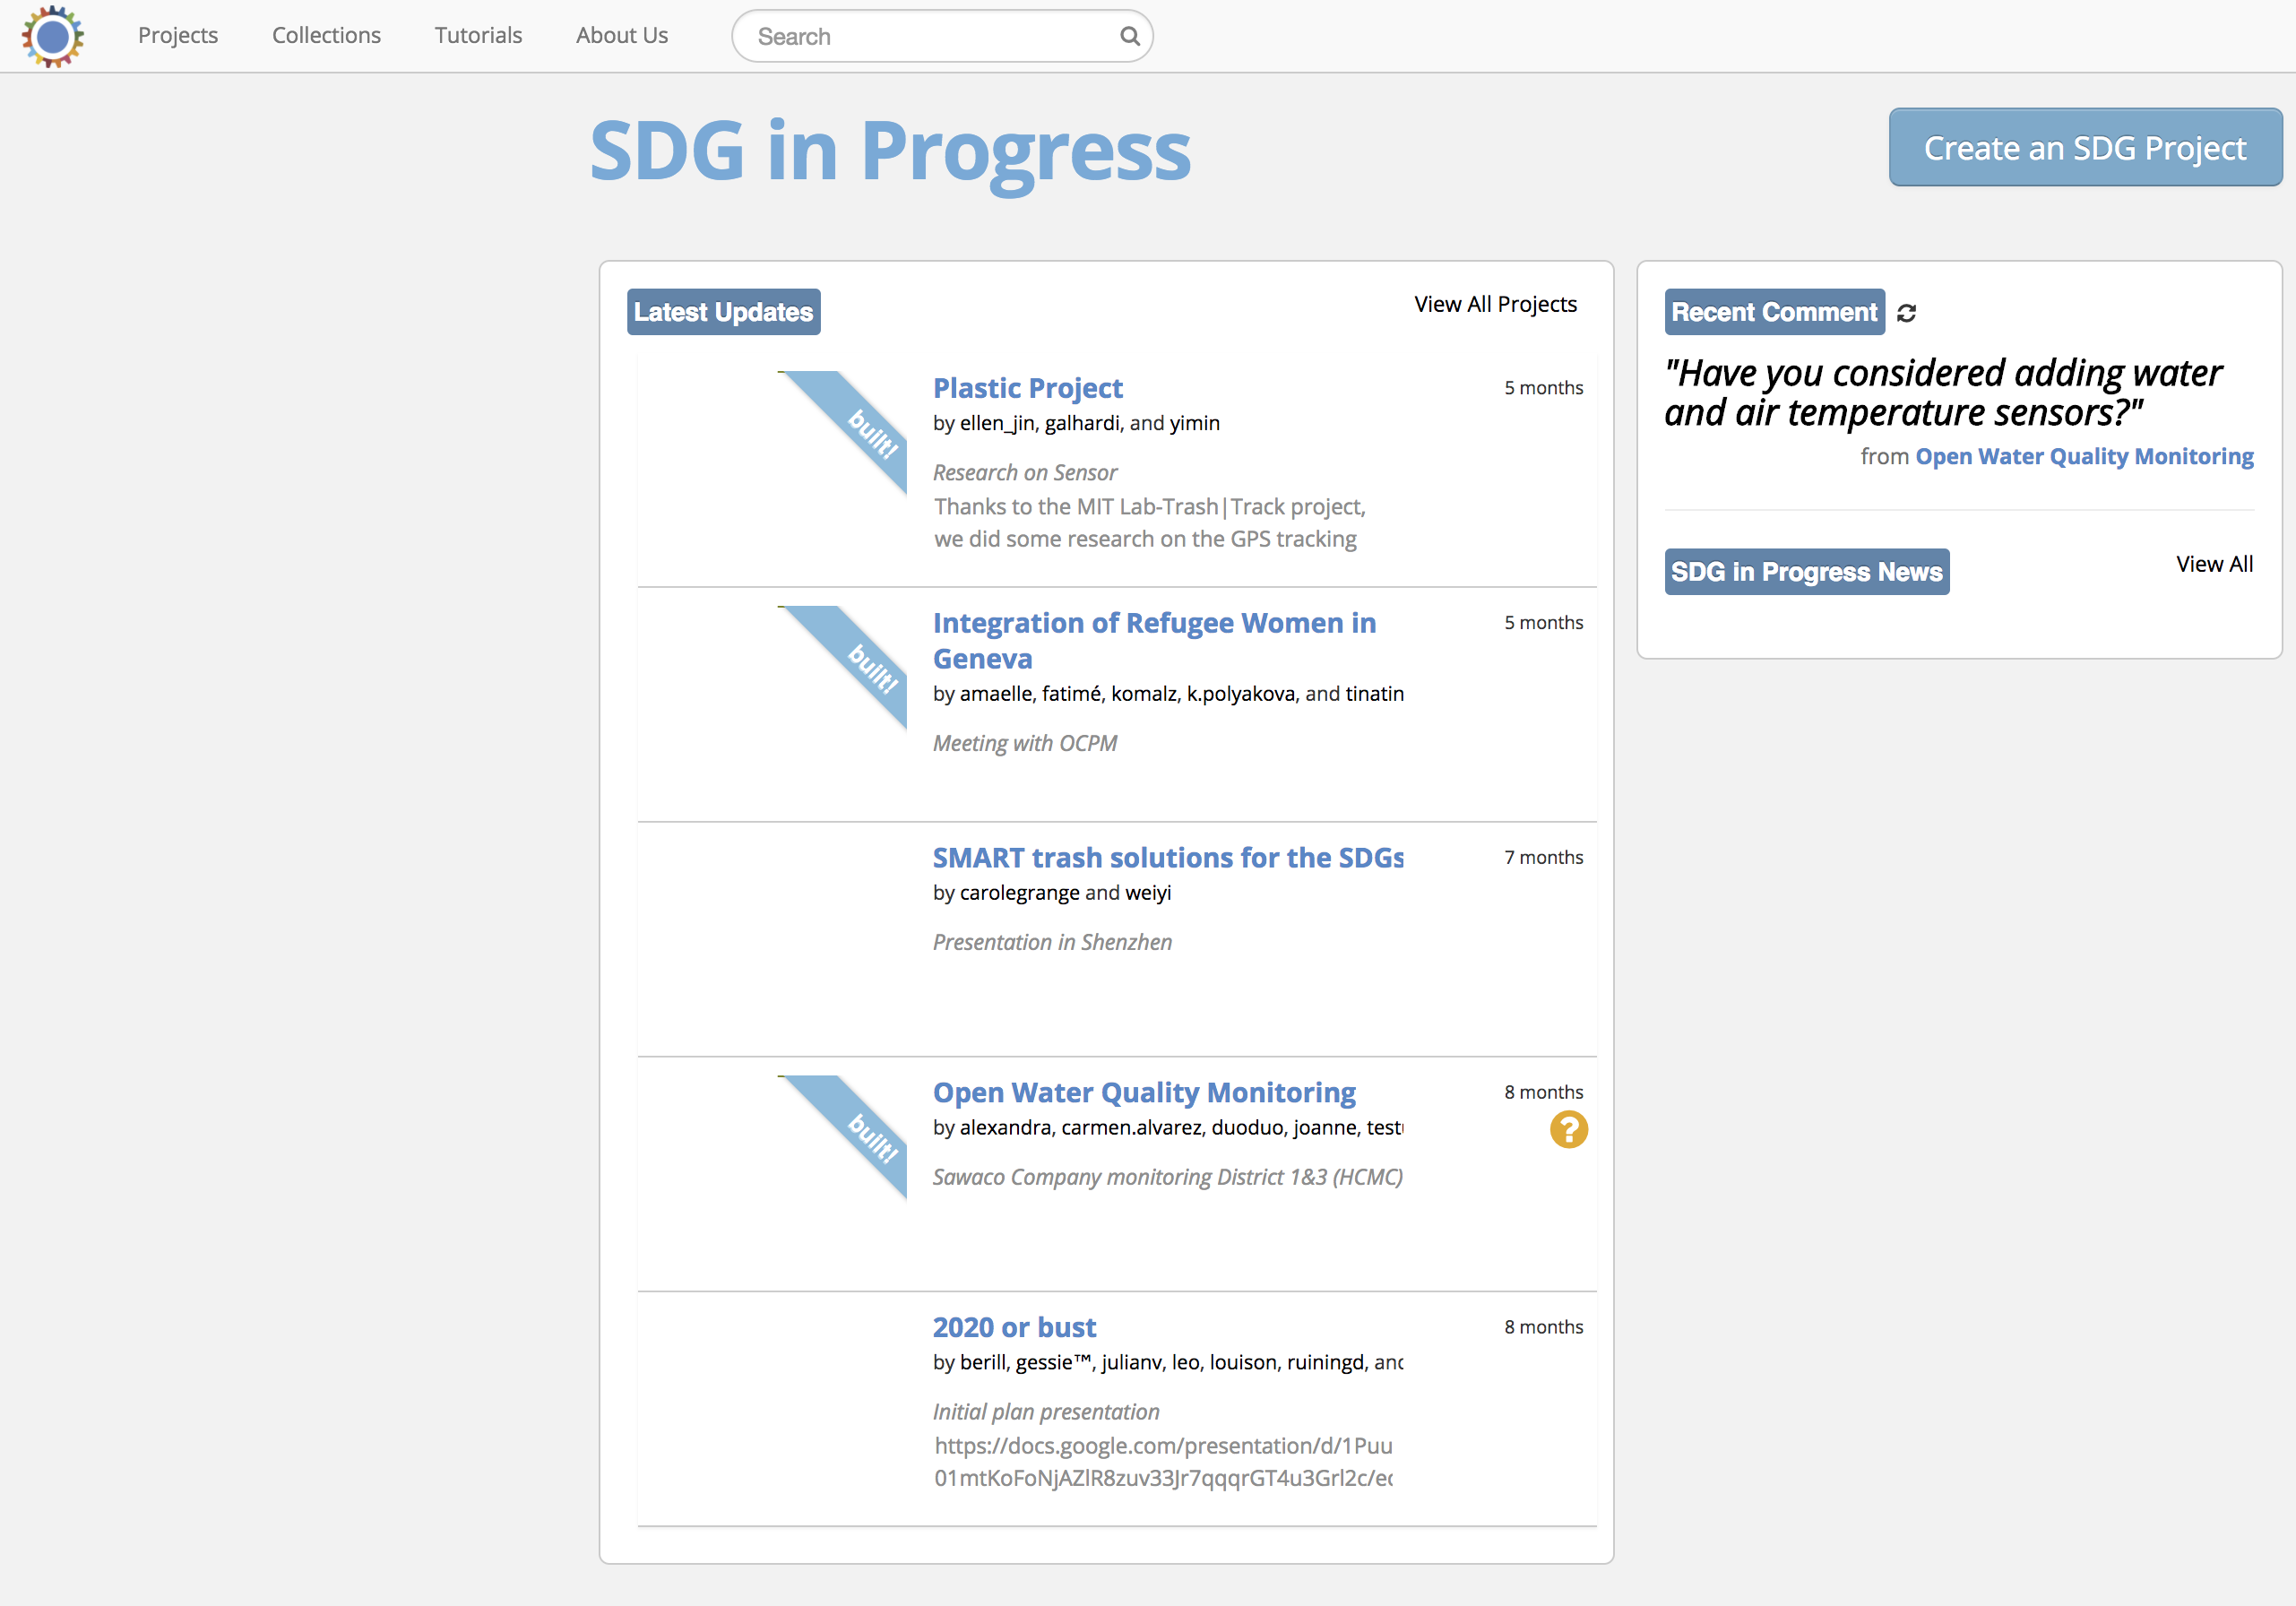
\includegraphics[width=15cm, height=10cm]{./images/img-sdginprogress.png}
	\caption{Build in progress welcome page}
	\label{img-sdginprogress}
\end{figure}

\subsection{Design approach}
Authors shared an iterative design process in the context of sharing their personal journey by creating step-by-step instructions of their project via the online platform \textit{SDGinProgress} and companion mobile application. Readers contributed by suggesting to makers after publishing their steps, makers benefited from sharing step-by-step instructions over time by taking into account the suggestions of readers.

SDGinProgress was developed based on an innovative design process, it enables users to visualize their documentation in an iterative way. Authors can continuously iterate their building process, share their techniques to help others to reach out others in the community so they can have feedback. A social design process principle was considered among the online community to engage users more, to accumulate knowledge, to learn from others and connect users with same interest as \textit{human-related issues in the form of social ties and knowledge sharing were reported as keys to successful collaboration} \cite{Kotlarsky2005}.

\subsection{Features}\label{sec:feature}
SDGinProgress consists of many features in the project page and social feature. The two core features of the project page are : the \textit{Process Map} and \textit{Step Detail View } (\ref{img-sdginprogressproject}).
\begin{figure}[ht!]
	\centering
	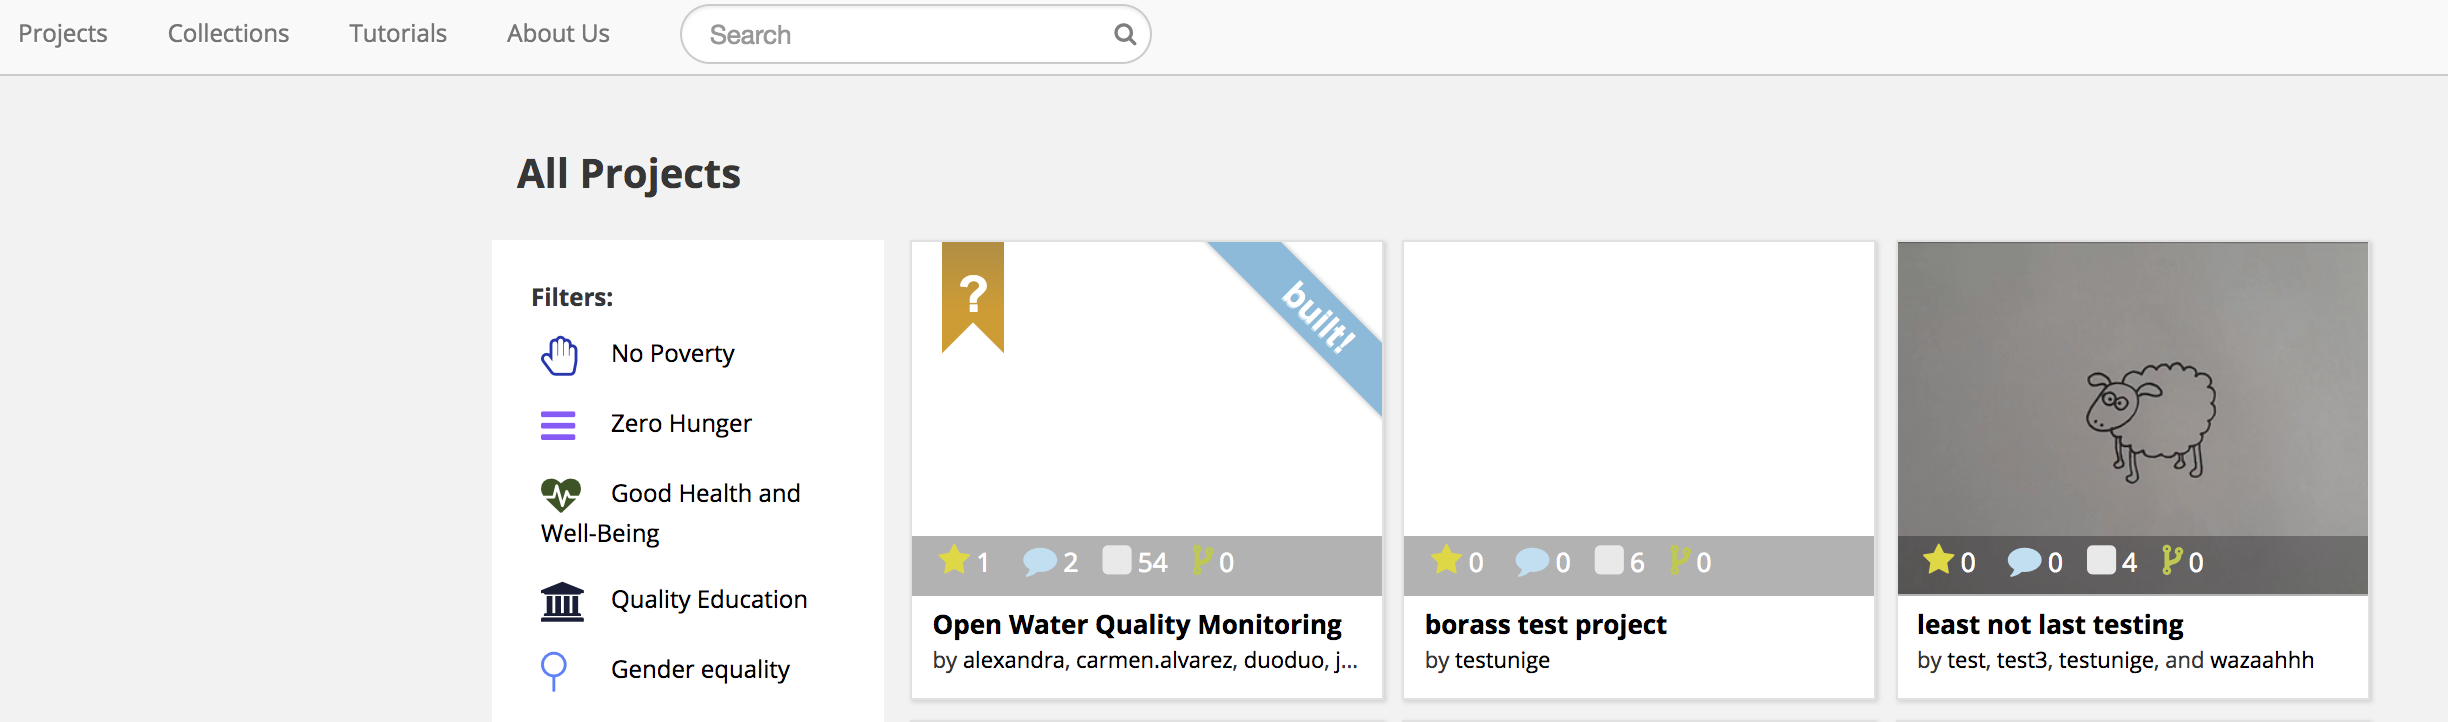
\includegraphics[width=.5\textheight]{./images/img-sdginprogressproject.png}
	\caption{overall project page view, [\url{https://sdginprogress.com/projects/81/steps}]} 
	\label{img-sdginprogressproject}
\end{figure}
In the process map, users can create a step, a label for one or more step, drag \& drop  to rearrange steps. Steps are organized in a tree-map-like format with sui generis branches, a label is added to a branch and it can be colored to designate a branch; for example orange labels represent that a branch is in progress.

Project are displayed in 3 different mode.  The first is the default mode : tree-map, users can go through all the steps, step-by-step and discover more about it as shown in figure \ref{img-viewtreemode1}.
\begin{figure}[H]
	\centering
	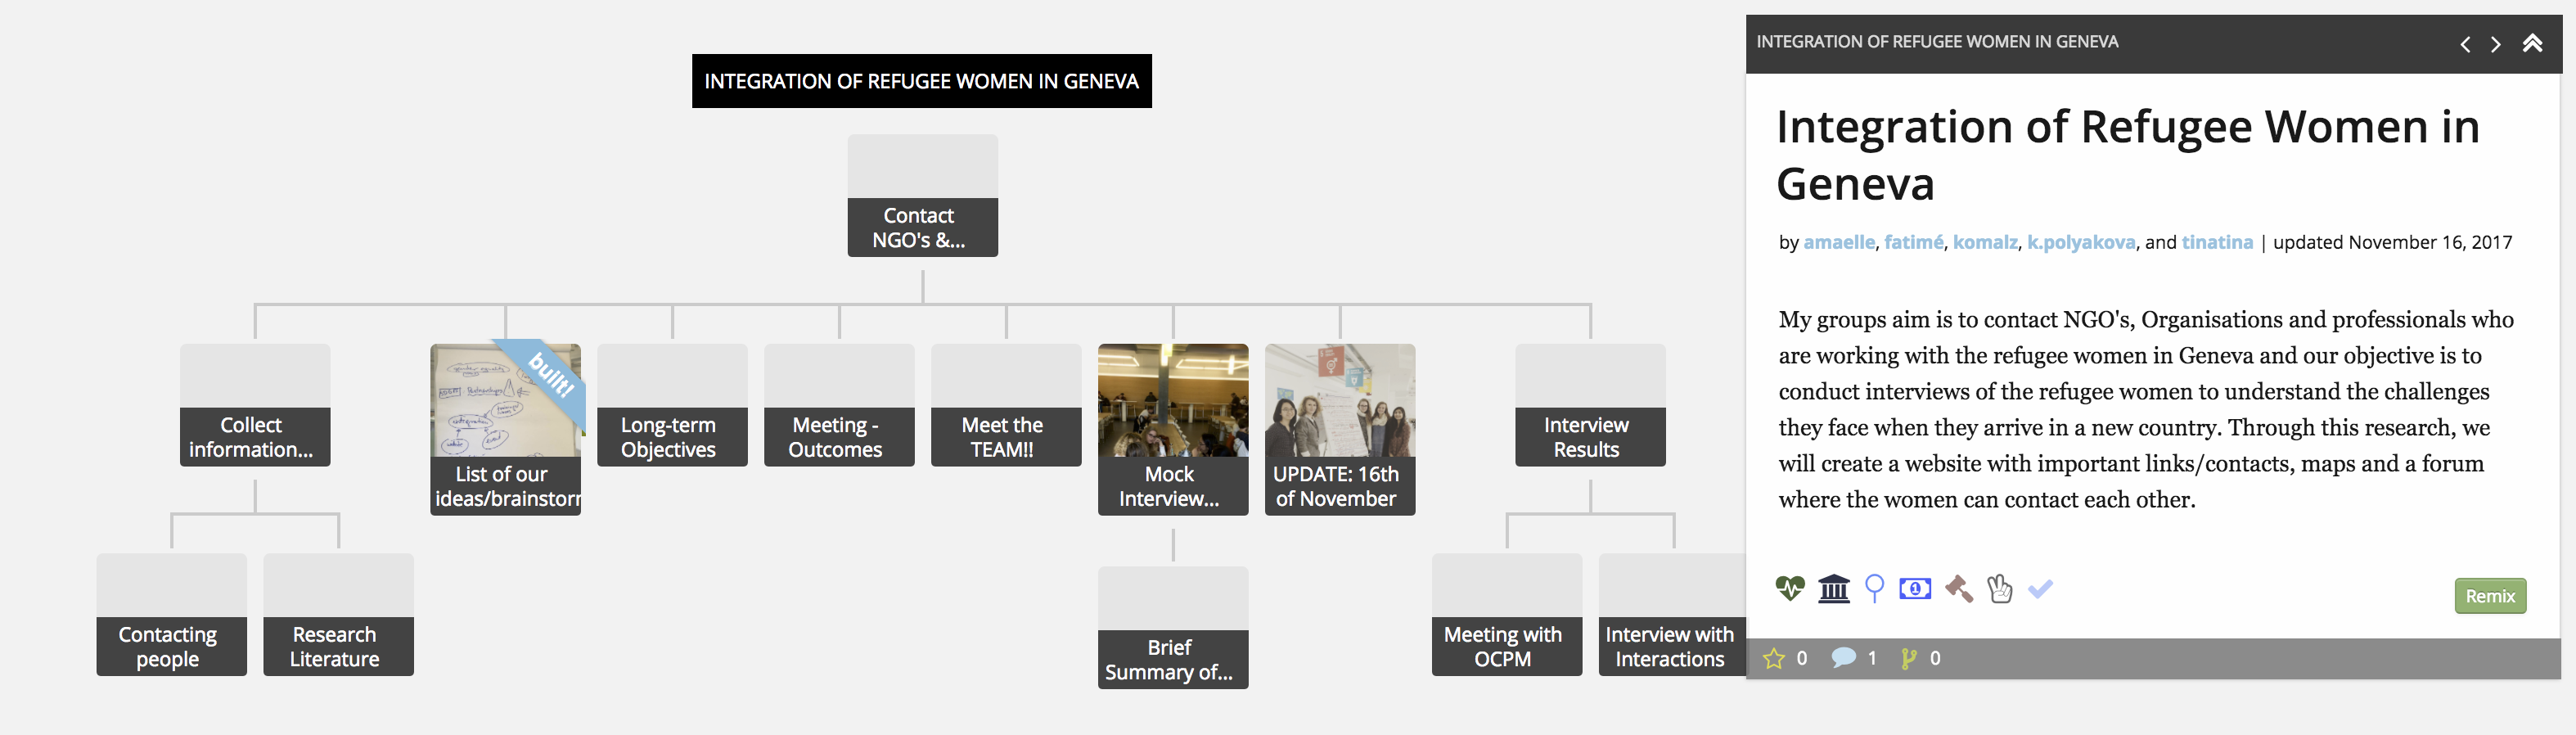
\includegraphics[scale=.25]{./images/img-refugeeintegration.png}
	\caption{tree-map view of the project} 
	\label{img-viewtreemode1}
\end{figure}

The second is Gallery mode \ref{img-viewgallerymode3} and finally  the  blog mode : users can scroll down and an index of steps will be displayed on their left side of the page (figure \ref{img-viewgallerymode3}).

\begin{figure}[H]
	\centering
	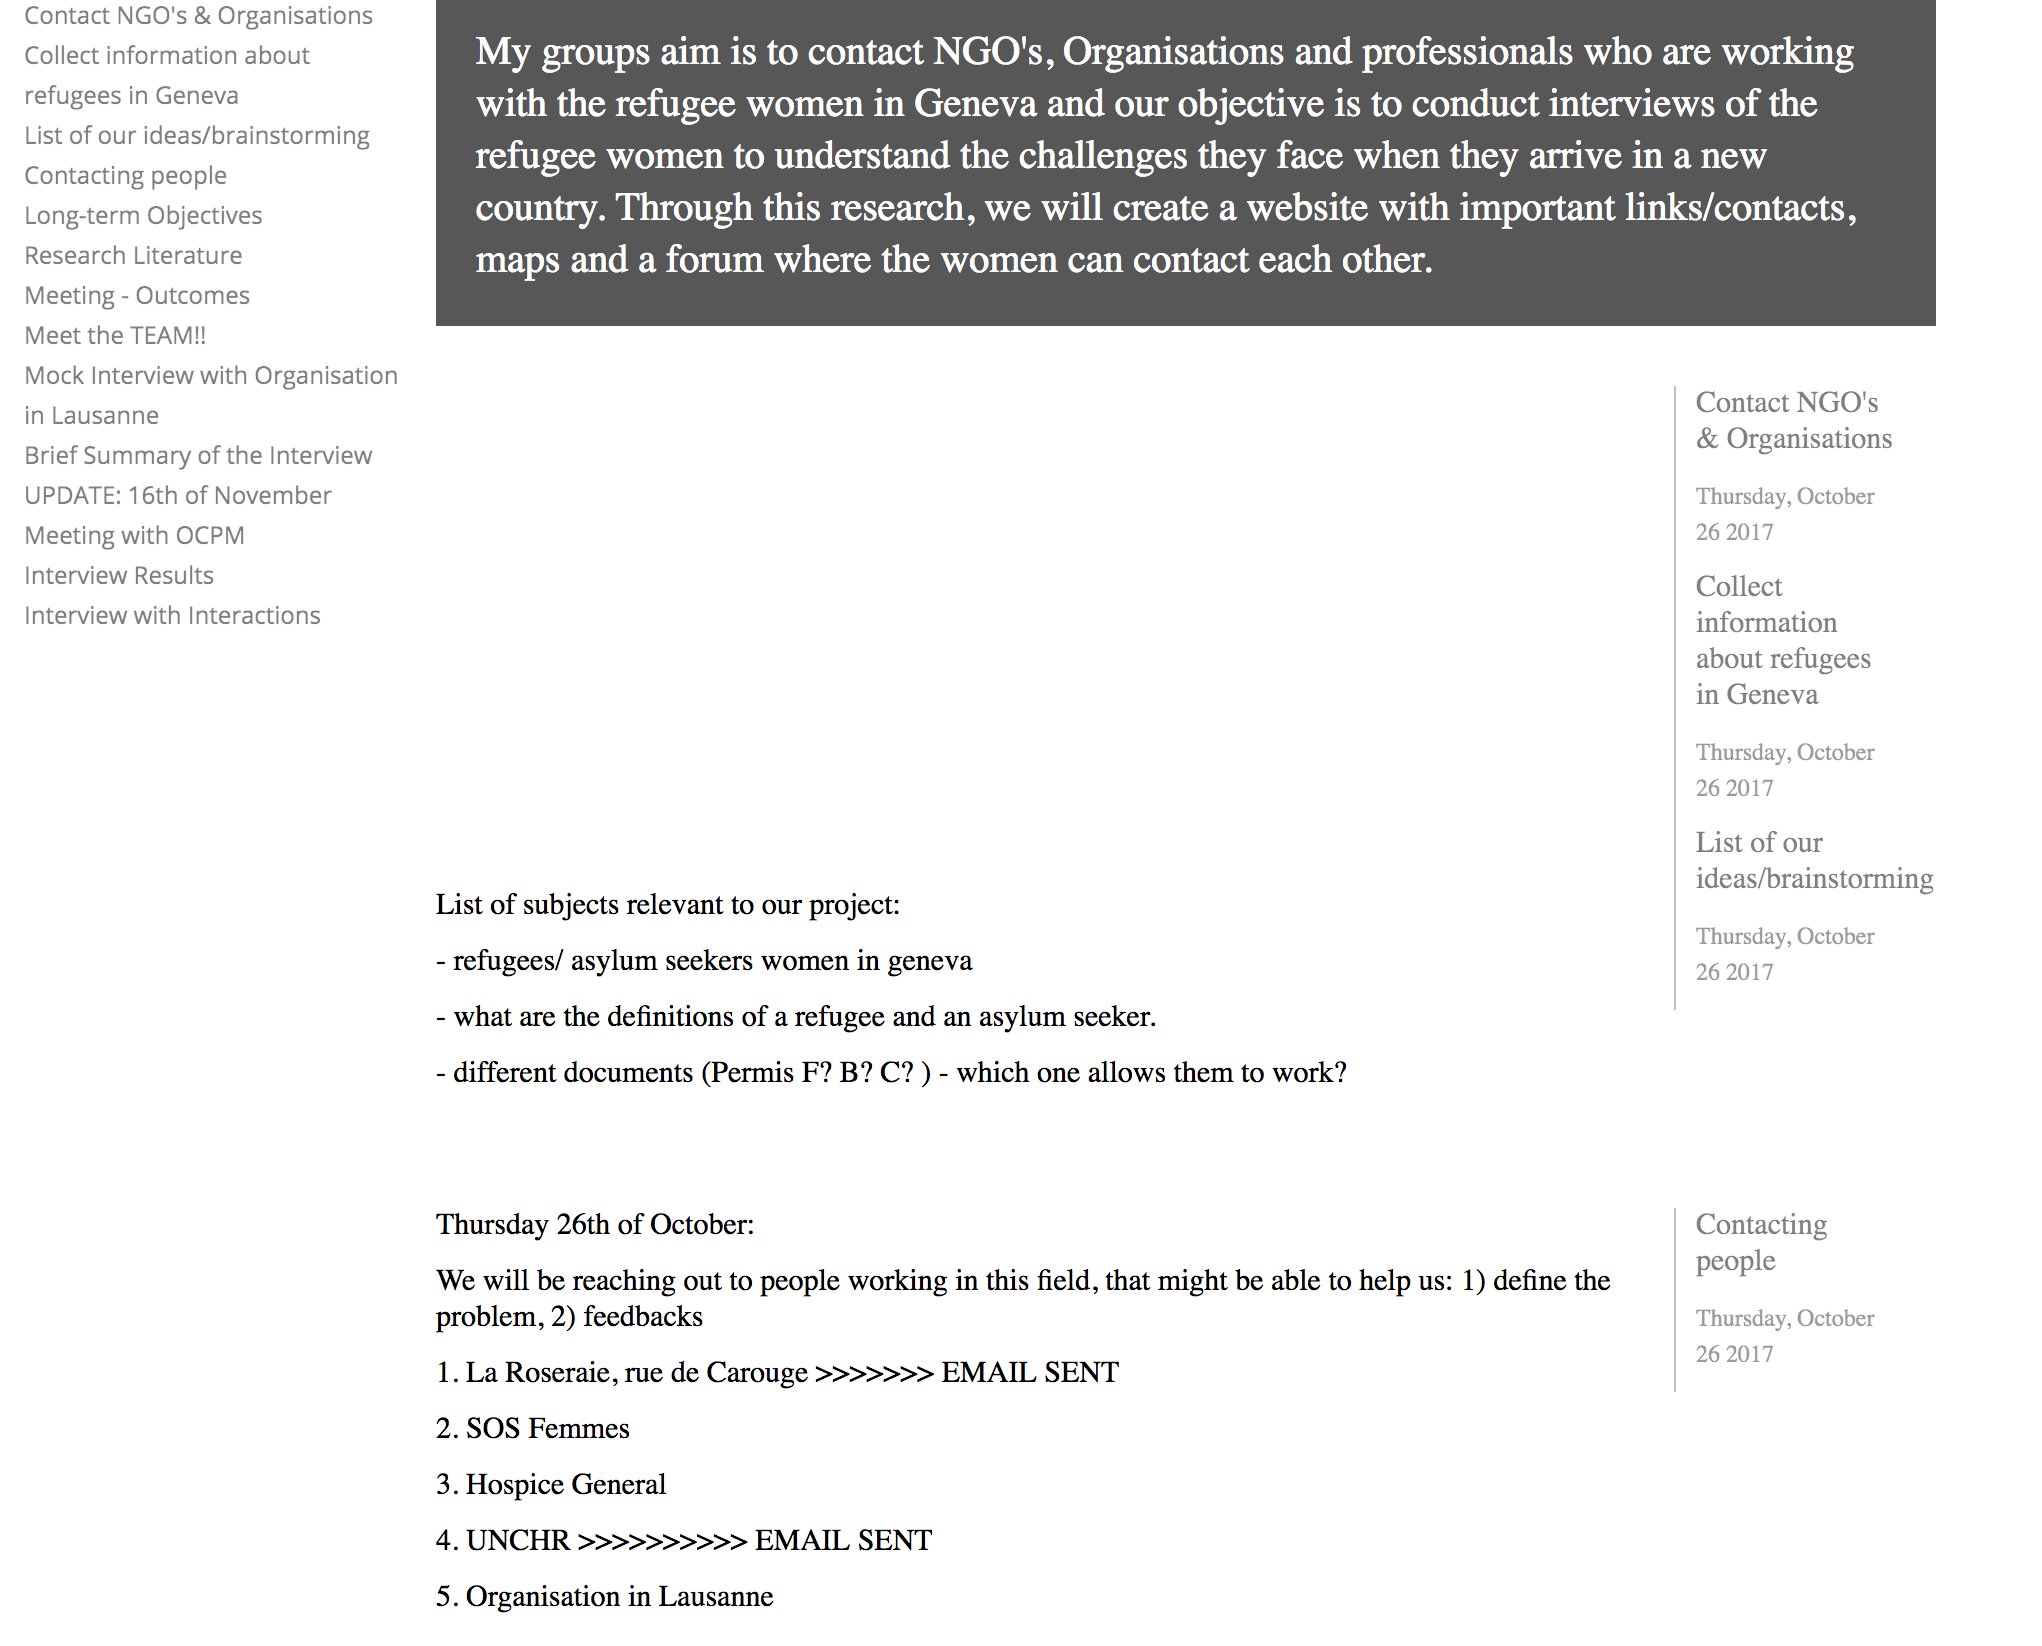
\includegraphics[scale=.3]{./images/img-refugeeintegrationblogmode.png}
	\caption{Gallery view of the project} 
	\label{img-viewgallerymode3}
\end{figure}

%\begin{figure}[H]
%	\centering
%	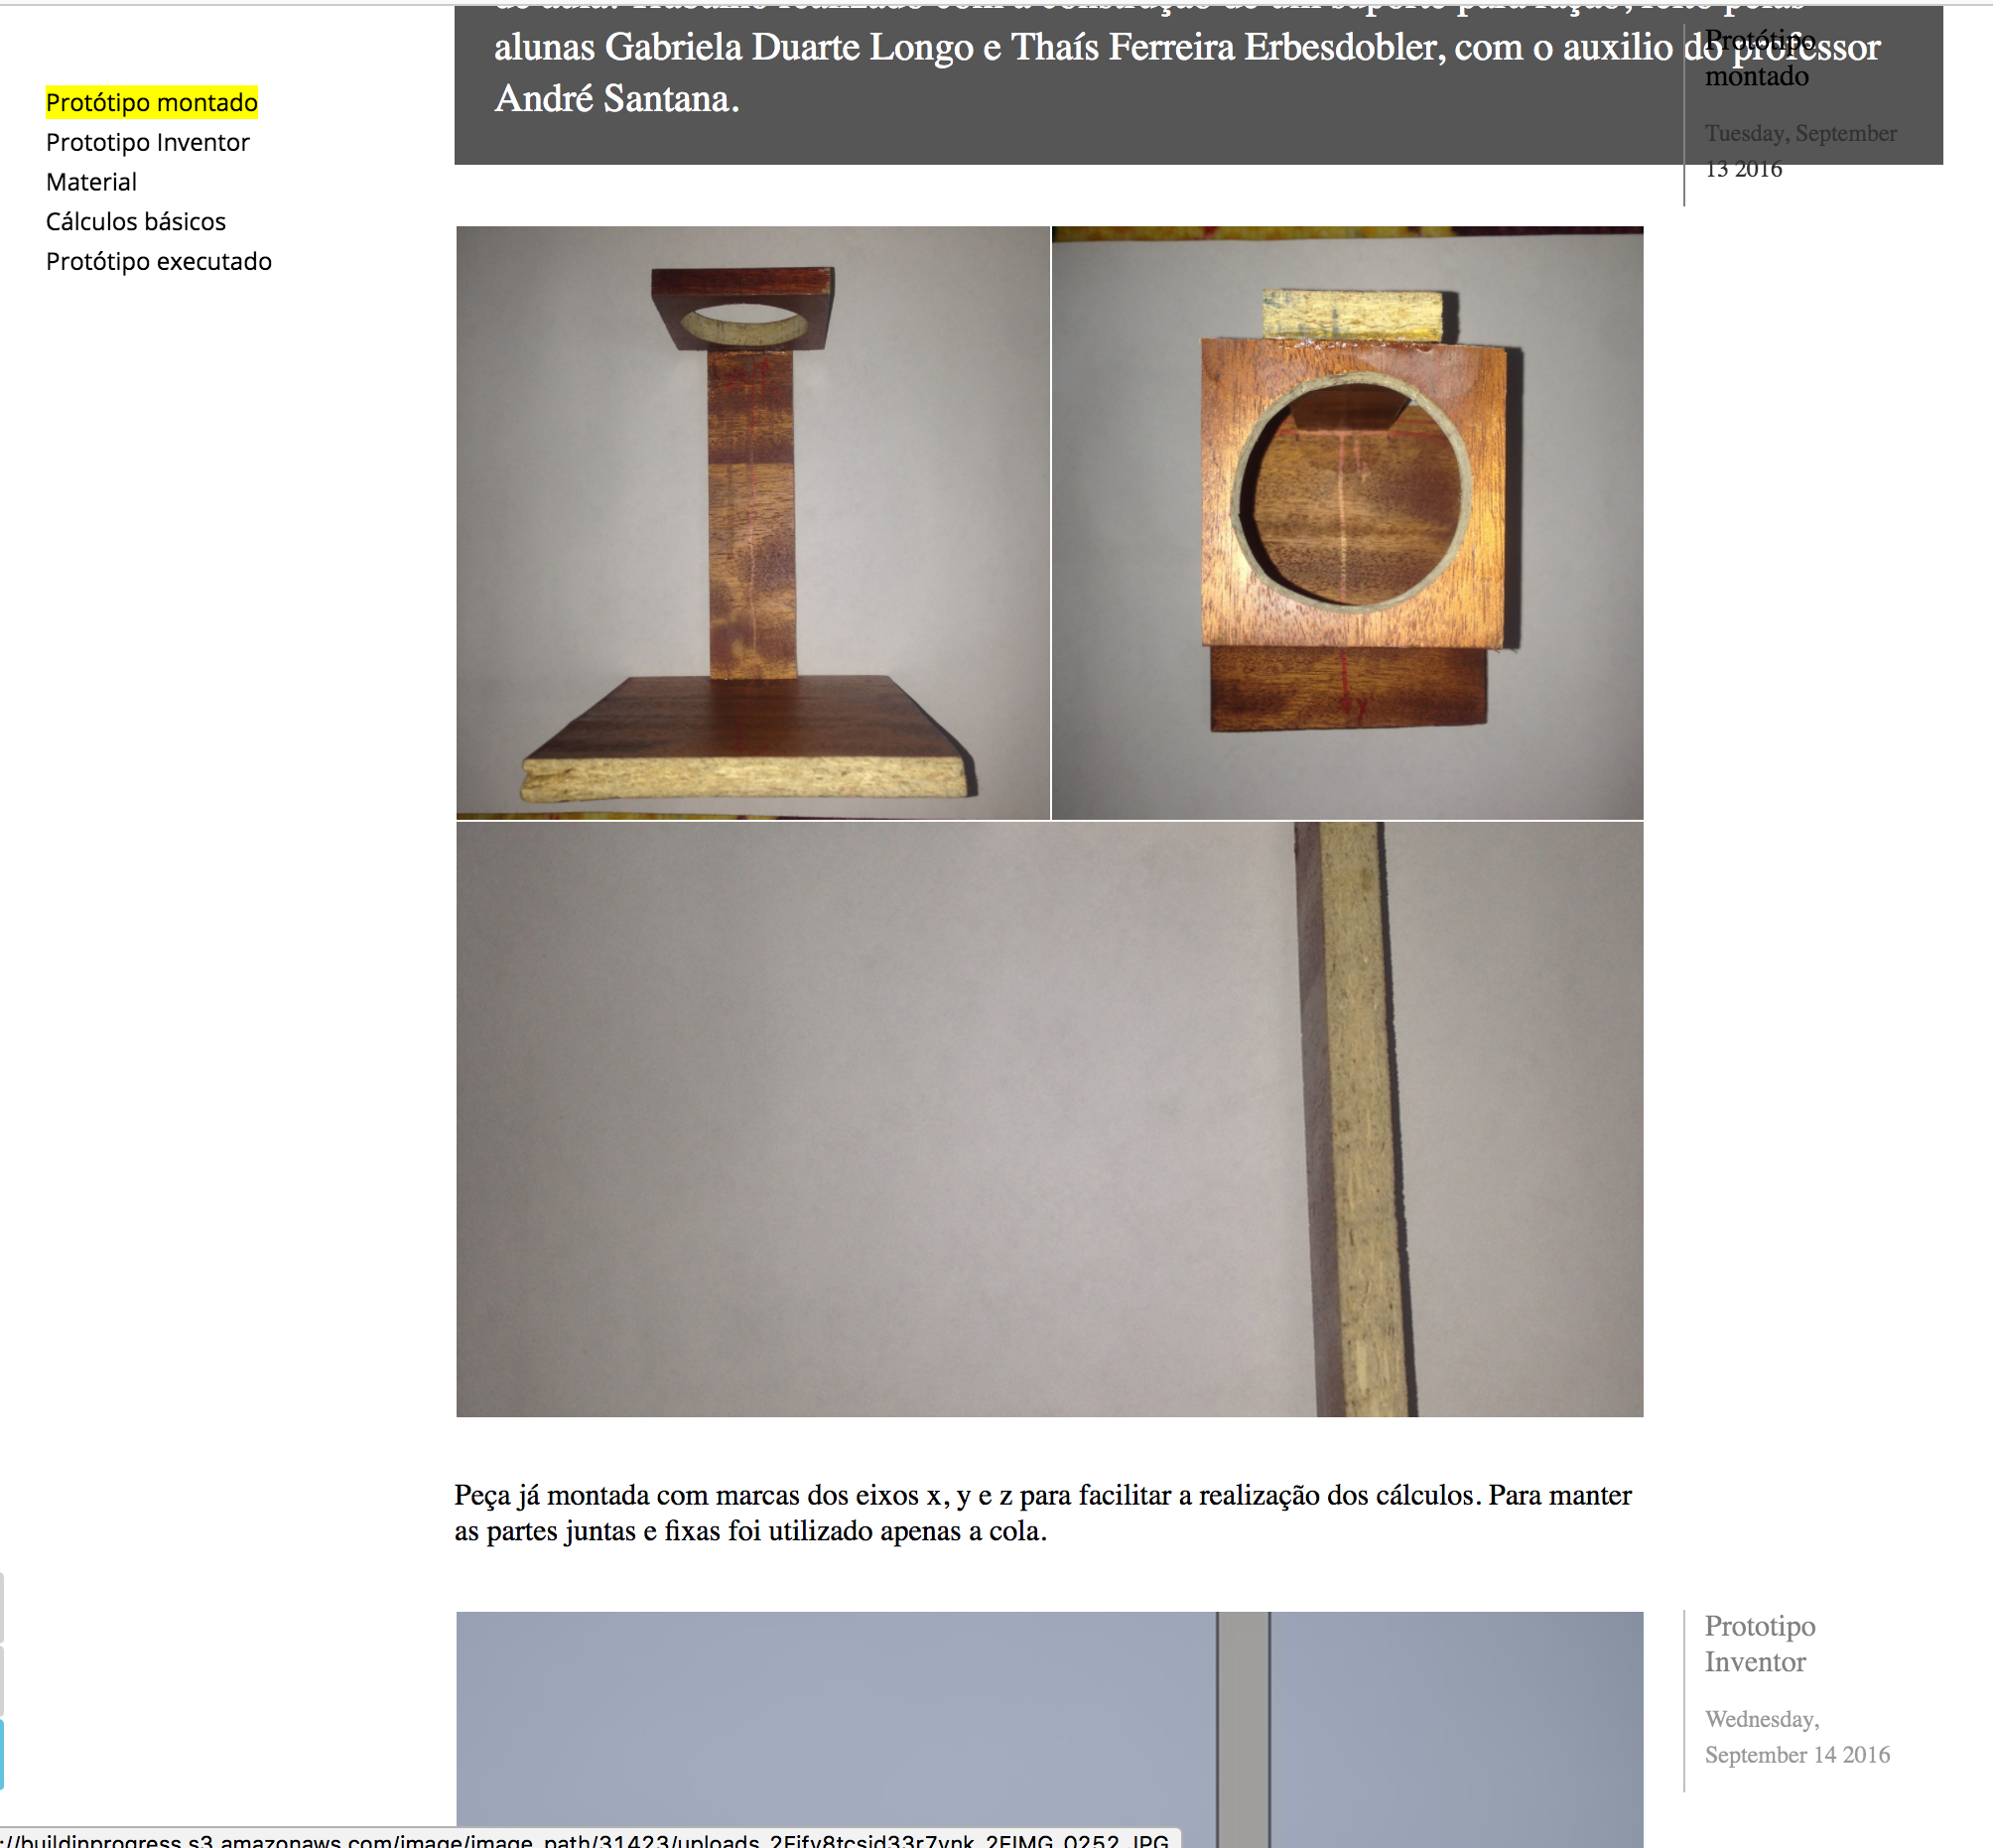
\includegraphics[scale=.3]{./images/img-mode3.png}
%	\caption{Blog like mode} 
%	\label{img-mode3}
%\end{figure}

In \textit{Details of step} users can upload photos or videos, add text description, ask others a question that will appear in the homepage of the platform, upload resources or files in different formats; e.g. .PDF, .PPT, a given example is shown in the figure \ref{img-stepdetails1} .
\begin{figure}[H]
	\centering
	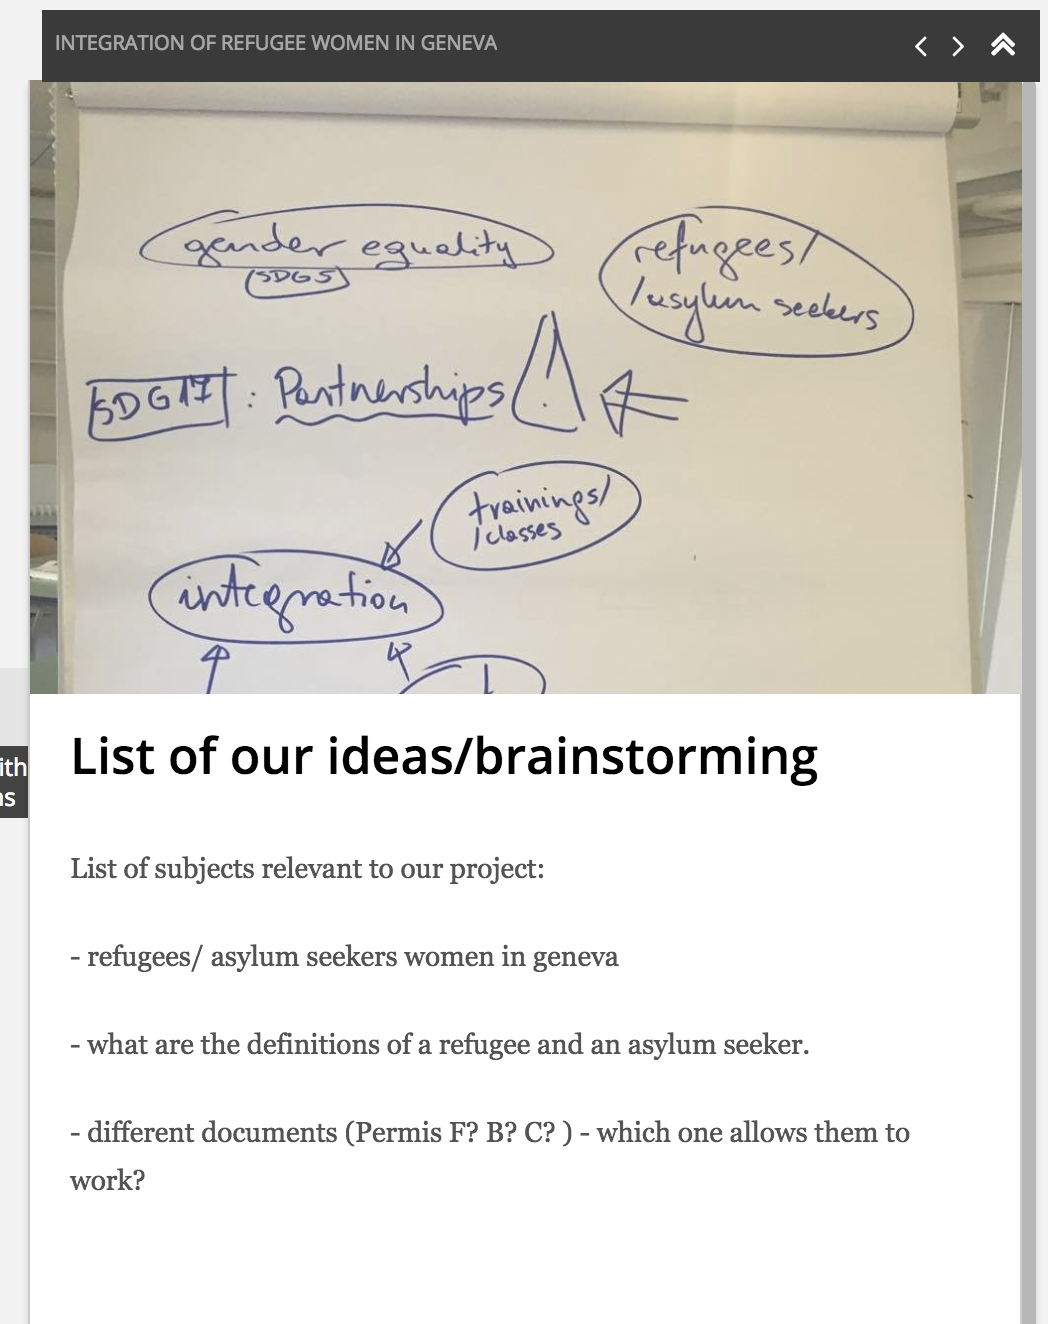
\includegraphics[scale=.3]{./images/img-stepdetails1.png}
	\caption{Details steps view} 
	\label{img-stepdetails1}
\end{figure}

The online platform incorporate many features that keep the SDGinProgress community more socialized and connected. Users can follow a project, see recent activity on the homepage and they will receive notification once an author add a step or ask a question.
\begin{figure}[H]
	\centering
	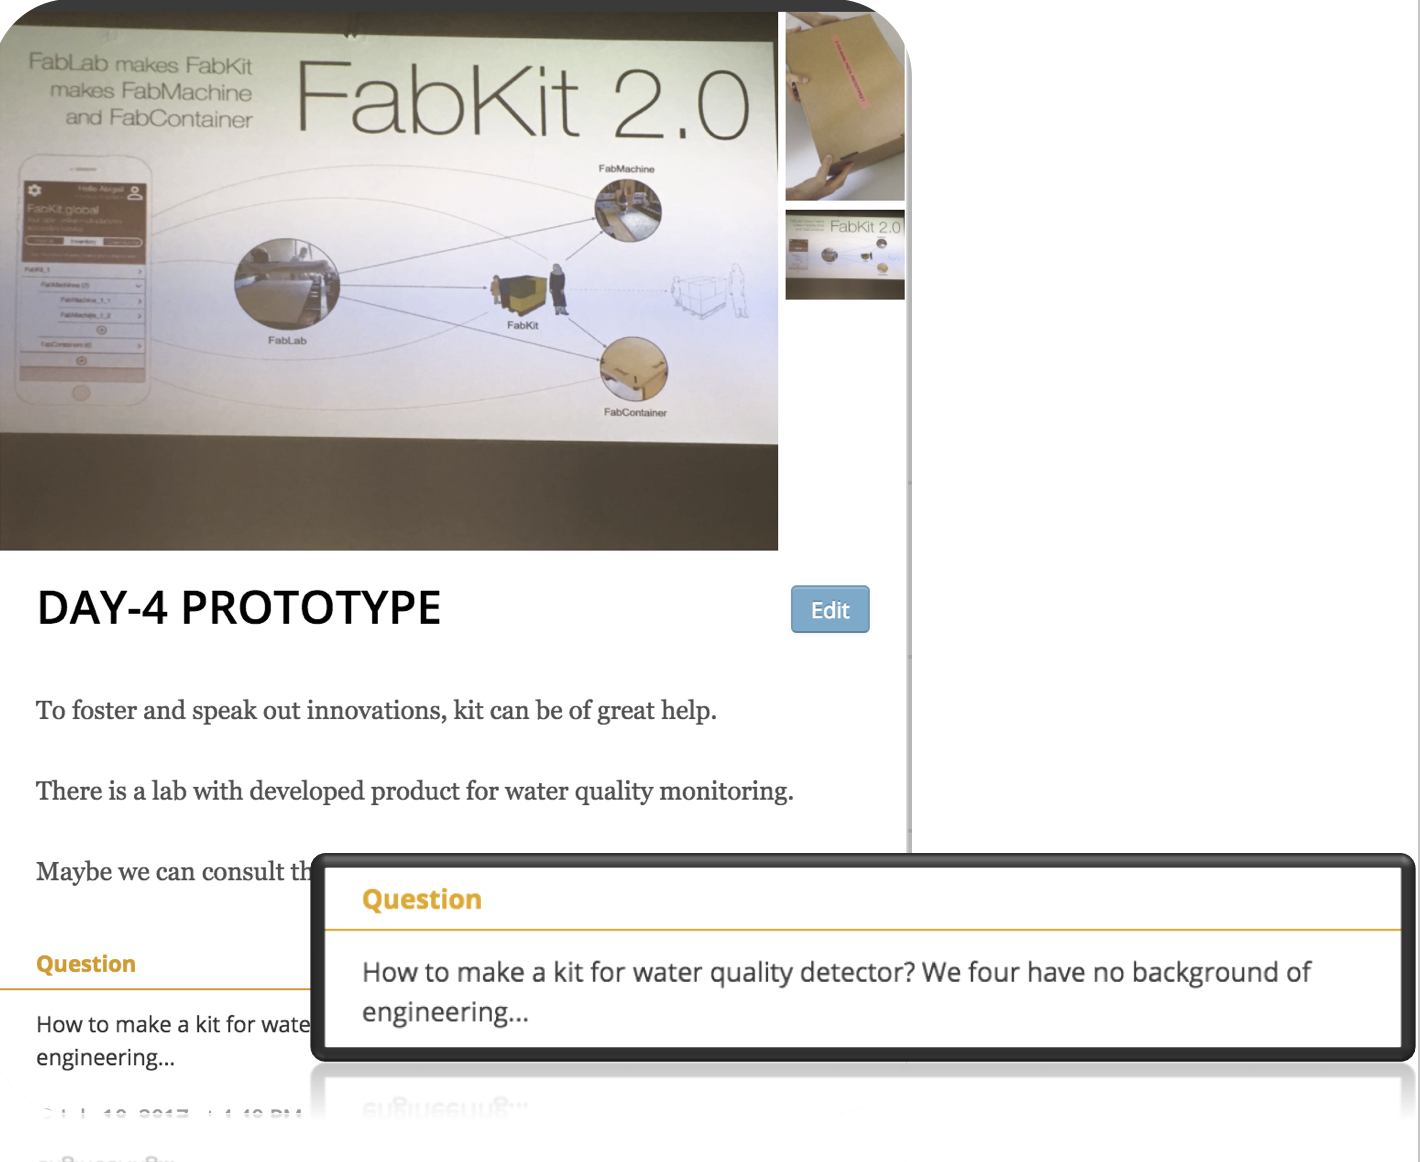
\includegraphics[scale=.4]{./images/img-commentquestion1.png}
	\caption{Question featured in the home page} 
	\label{img-commentquestion}
\end{figure}

Moreover, users can leave a text on any step and they will receive a notification when a comment is left. Authors can ask for feedback or help by embedding a question that will be added to the Community Activity section of the homepage, see figure \ref{img-commentquestion}.
\subsubsection{Mobile application}
A mobile application has been created to make documentation more efficient in which users upload images and videos to their projects directly from their devices instead of taking picture from their devices then transfer it to a computer and upload it (figure \ref{img-mobileapp}). But in our experience with the summer school we didn't used it.
\begin{figure}[H]
	\centering
	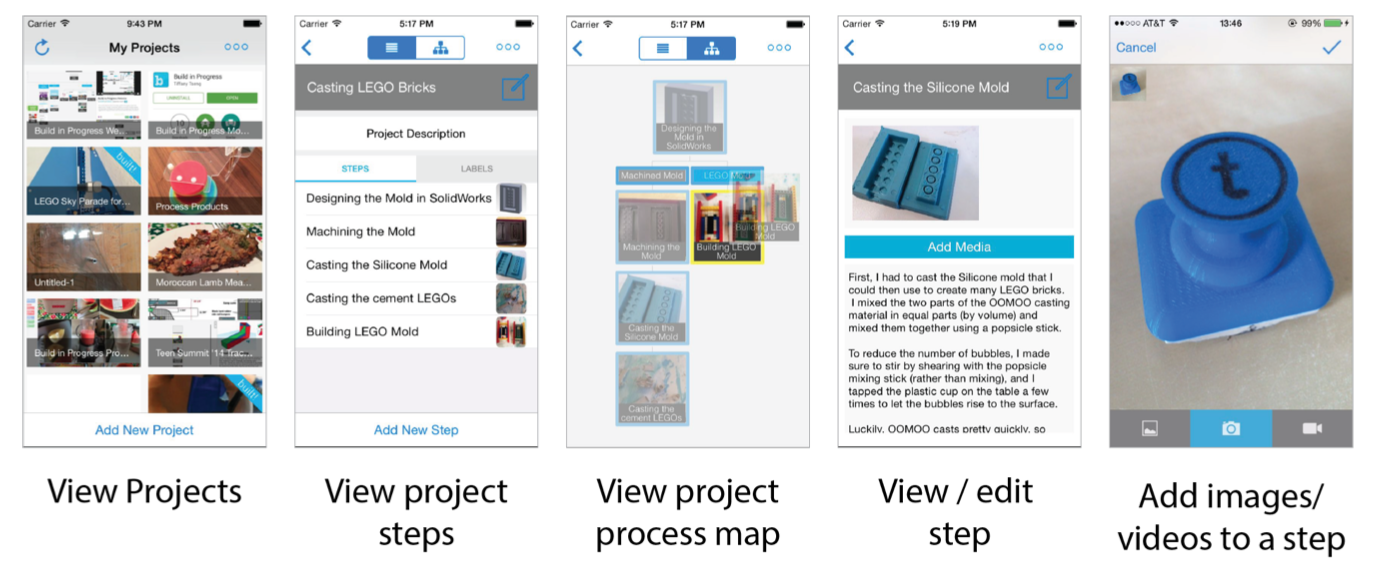
\includegraphics[scale=.5]{./images/img-mobileapp.png}
	\caption{Mobile application interface, [Tseng, 2016]} 
	\label{img-mobileapp}
\end{figure}


\section{Use of SDG}
\todo[inline]{How many teams used it, what they usd it for}
\todo[inline]{Quote some feedback if it is written or recorded}

\subsection{User interaction}
SDGinProgress has been used in summer-school programs and in after-summer-school by students who work on their own project. Teenagers and one adult facilitator have been interviewed and a weekly interview has been done to all teams to get an estimation about their weekly hours work.

The results of the interviews and surveys showed that users get motivated to share their project at the beginning as it facilitate getting a feedback of what they have done, create and show their portfolio projects, get engaged to document and to help others. Users were divided into two opinions, one part of the students found that SDGinProgress support meaningful documentation practices and the second part of the students found that it doesn't support their project the latter are typically software development project or policy making. Many strategies were identified depending on the type of project, the duration of a project and the age of makers who are using it.

\subsection{Summary}

The study of SDGnProgress showed that it support authors and readers but it has some limitation. The documentation help students to create a design process for their project by learning from the many iterations they did over time and SDGnProgress motivates reflective practice on making, design process, and values and identity. Users get engaged, get feedback, and help others. SDGinProgress support all capturing way written and visual. \textcolor{red}{In our experiments} The platform SDGinProgress helped students to document their project and it gaves them the opportunity to win visibility and get feedback from others, for example, as we see in the picture below. 
\begin{figure}[ht!]
	\centering
	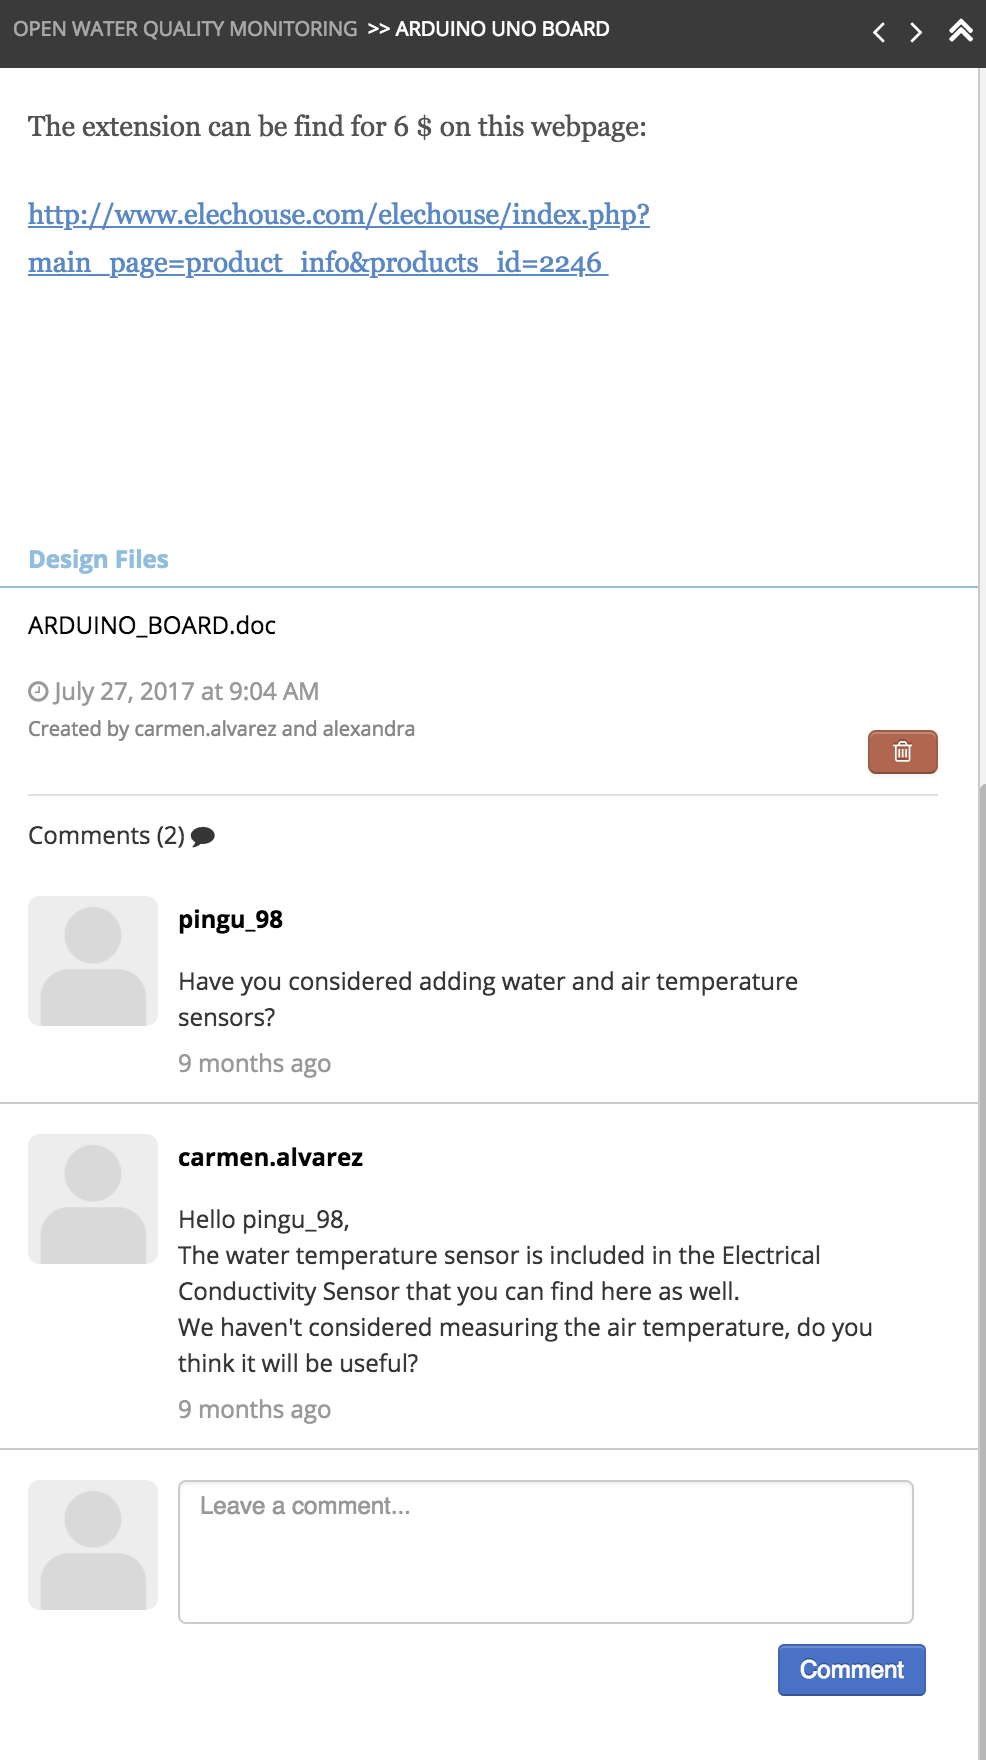
\includegraphics[width=.3\textheight]{./images/img-cmtsdgip.png}
	\caption{Comments and feedbacks on a hardware ste, \cite[\url{https://sdginprogress.com/projects/47/steps?comment_id=4&notification_id=442&step=214}]{SDGdinP1}} 
	\label{img-cmtsdgip}
\end{figure}
An engineer from CERN is giving them a comment about their hardware, others were asking question to the public to get some ideas. so the use of the platform overall is good for documentation but there is a lack of incentive for writing. Student tend to postpone documentation then forget what they want to document, which lead to weak documentation that give the big outline about a project and it doesn't really help if someone else want to copy the project






\section{Discussion}

\textit{SDGinProgress} and \textit{Instructables} didn't bring a new fundamental way in which users can share their captured media publicly or in private. Design parameters can be adjusted to support different type of users-interactions and goals.  Instructables enable users to personalize through substitution and modification of a step and any missing step mean that authors should re-create their documentation while BiP focus more on the  design process where users can iterate their project by creating new branches and forget about the unsuccessful branches.

The mix between capturing and text-based-description features in SDGinProgress enables teenagers to document. The ease of use for creating a branch, drag \& drop simplify the job for younger audience especially readers who are new to the community of \textit{DIY} as they can go through steps, iterate on their work, modify a step or re-arrange some steps.  Instructables has both features but there is no friendly structure where authors get their documentation organized and if an author has a limited background in documentation or he doesn't like it, he will probably abandon the documentation of a project after the first type a user find that it is not possible to re-arrage the documented steps.

Sharing a project is not enough for authors. Users in Instructables found that they cannot share their thought or it is limited as the only way to express what they think is via a comment. SDGinProgress offers a text-based option where both authors and readers could ask a question or leave a comment, also, both can receive a notifications for a reply from the community or any other news concerning any modification in the project.

The process of sharing the effort in progress enable users to communicate more in BiP, they helped each other, they showed their effort, they get featured and receive feedback as described in section \ref{sec:feature}. Balancing the ease of use of automated documentation systems with the powerful feature, a mobile application, encourage more users to upload pictures or videos and enable them to be physically free so they can move around to document their project for example without having the problem of taking a photo, remember which step it is, transfer it then upload it to the platform as in Instructables.
\chapter{Hackathons}
% We're going to need an extra theorem-like environment for this
% chapter
\theoremstyle{plain}
\theoremsymbol{}
\newtheorem{Rule}[theorem]{Rule}

\begin{comment}
%%  A structure to follow in each section

% Abstract
\section{Abstract}

% Introduction
\section{Introduction}

%% Central Report Section
% Methodology
\section{Methodology (what you did/used)}

% RESULTS
\section{RESULTS (what you found/saw)}

% DISCUSSION/CONCLUSION
\section{DISCUSSION/CONCLUSION}

\renewcommand{\labelenumii}{\Roman{enumii}}
\begin{enumerate}

	\item  

\end{enumerate}
\end{comment}

%% Start Here 

\section{Abstract}
\Rule{What is it ?}
How it works in hackathons with people from different backgrounds, how ideas get generated and how people document their hackathons ?
\section{Introduction}

\section{Methodology (what you did/used)}

\section{RESULTS (what you found/saw)}

\section{DISCUSSION/CONCLUSION}

\renewcommand{\labelenumii}{\Roman{enumii}}
\begin{enumerate}

	\item Summarize experience of hackathons / personal point of view
	\item Write about this experience and what you came out with
		\item Write about this experience and what you came out with, and how the hackathons shaped the innovation

\end{enumerate}
\textit{How the follow up works ? how team continues to work ? how ideas progress over time ? how participants connect ?}


%%% Local Variables:
%%% mode: latex
%%% TeX-master: "thesis"
%%% End:
\textcolor{red}{\chapter{Summer School}

\section{Summer school projects}
\label{sec:scprojects}


\section{Summer school teams}
\label{sec:scteams}


\section{Summer school documentation}
\label{sec:scdocumentation}}

%\chapter{SDG in Progress}
What motivate people to document or write ..

\section{What is it ?}

\section{Technical installation}

\section{Adapting SDG in Progress}

\section{Why use of SDG in Progress}
Characteristic of SDG in Progress
\section{Comparision with other platforms}

%%% Local Variables:
%%% mode: latex
%%% TeX-master: "thesis"
%%% End:

%\chapter{RoboDoc}

\section{The concept of the robot Assistant}
\label{sec:robotassistant}

bla bla bla

\section{How it work}
Put a conception model of it

do we need it ?

Why we need it ?

Put a conception model of it
\subsection{Experience 1 }

\subsubsection{Results of Experience 1}

\begin{description}
	\item[First step ] bla bla bla
	\item[Second ]  
	
\end{description}

\subsection{Experience 2 }
\begin{description}
	\item[First step ] bla bla bla
	\item[Second ]  
	
\end{description}
\subsubsection{Results of Experience 2}


\subsection{findings}
Here goes the conclusion of this experiments
%\chapter{Intencive of writing}
What motivate people to document or write ..

\section{Why documenting ?}

\section{Why it is important ?}

\section{How to motivate people to write ?}
%%% Local Variables:
%%% mode: latex
%%% TeX-master: "thesis"
%%% End:

\chapter{Conclusion}
%\chapter{Shape of a research article or thesis}
%%  A structure to follow in each section

% Abstract
\section{Abstract}

% Introduction
\section{Introduction}

%% Central Report Section
% Methodology
\section{Methodology (what you did/used)}

% RESULTS
\section{RESULTS (what you found/saw)}

% DISCUSSION/CONCLUSION
\section{DISCUSSION/CONCLUSION}

\begin{center}
	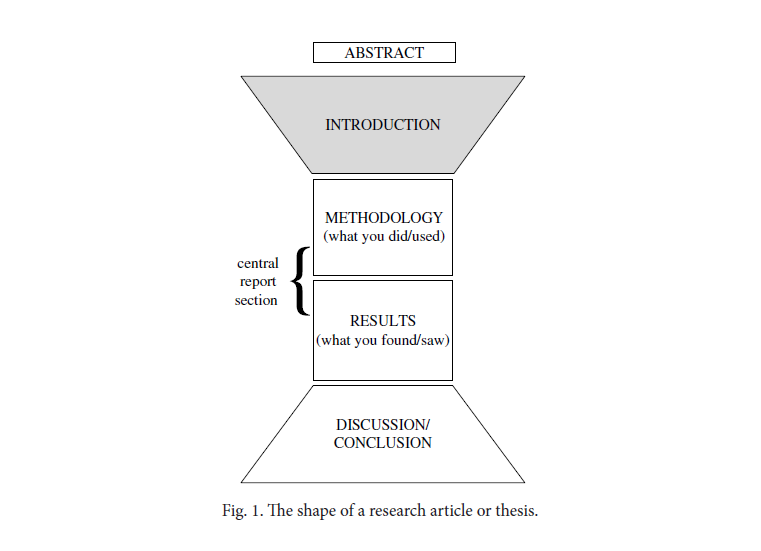
\includegraphics[scale=0.9]{./images/shapeofresartorthesis.png}
\end{center}
%% \chapter{Example Chapter}

Dummy text.

\section{Example Section}

Dummy text.

\subsection{Example Subsection}

Dummy text.

\subsubsection{Example Subsubsection}

Dummy text.

\paragraph{Example Paragraph}

Dummy text.

\subparagraph{Example Subparagraph}

Dummy text.


\appendix

%\chapter{Dummy Appendix}

You can defer lengthy calculations that would otherwise only interrupt
the flow of your thesis to an appendix.


\backmatter

\bibliographystyle{plain}
\bibliography{refs}

%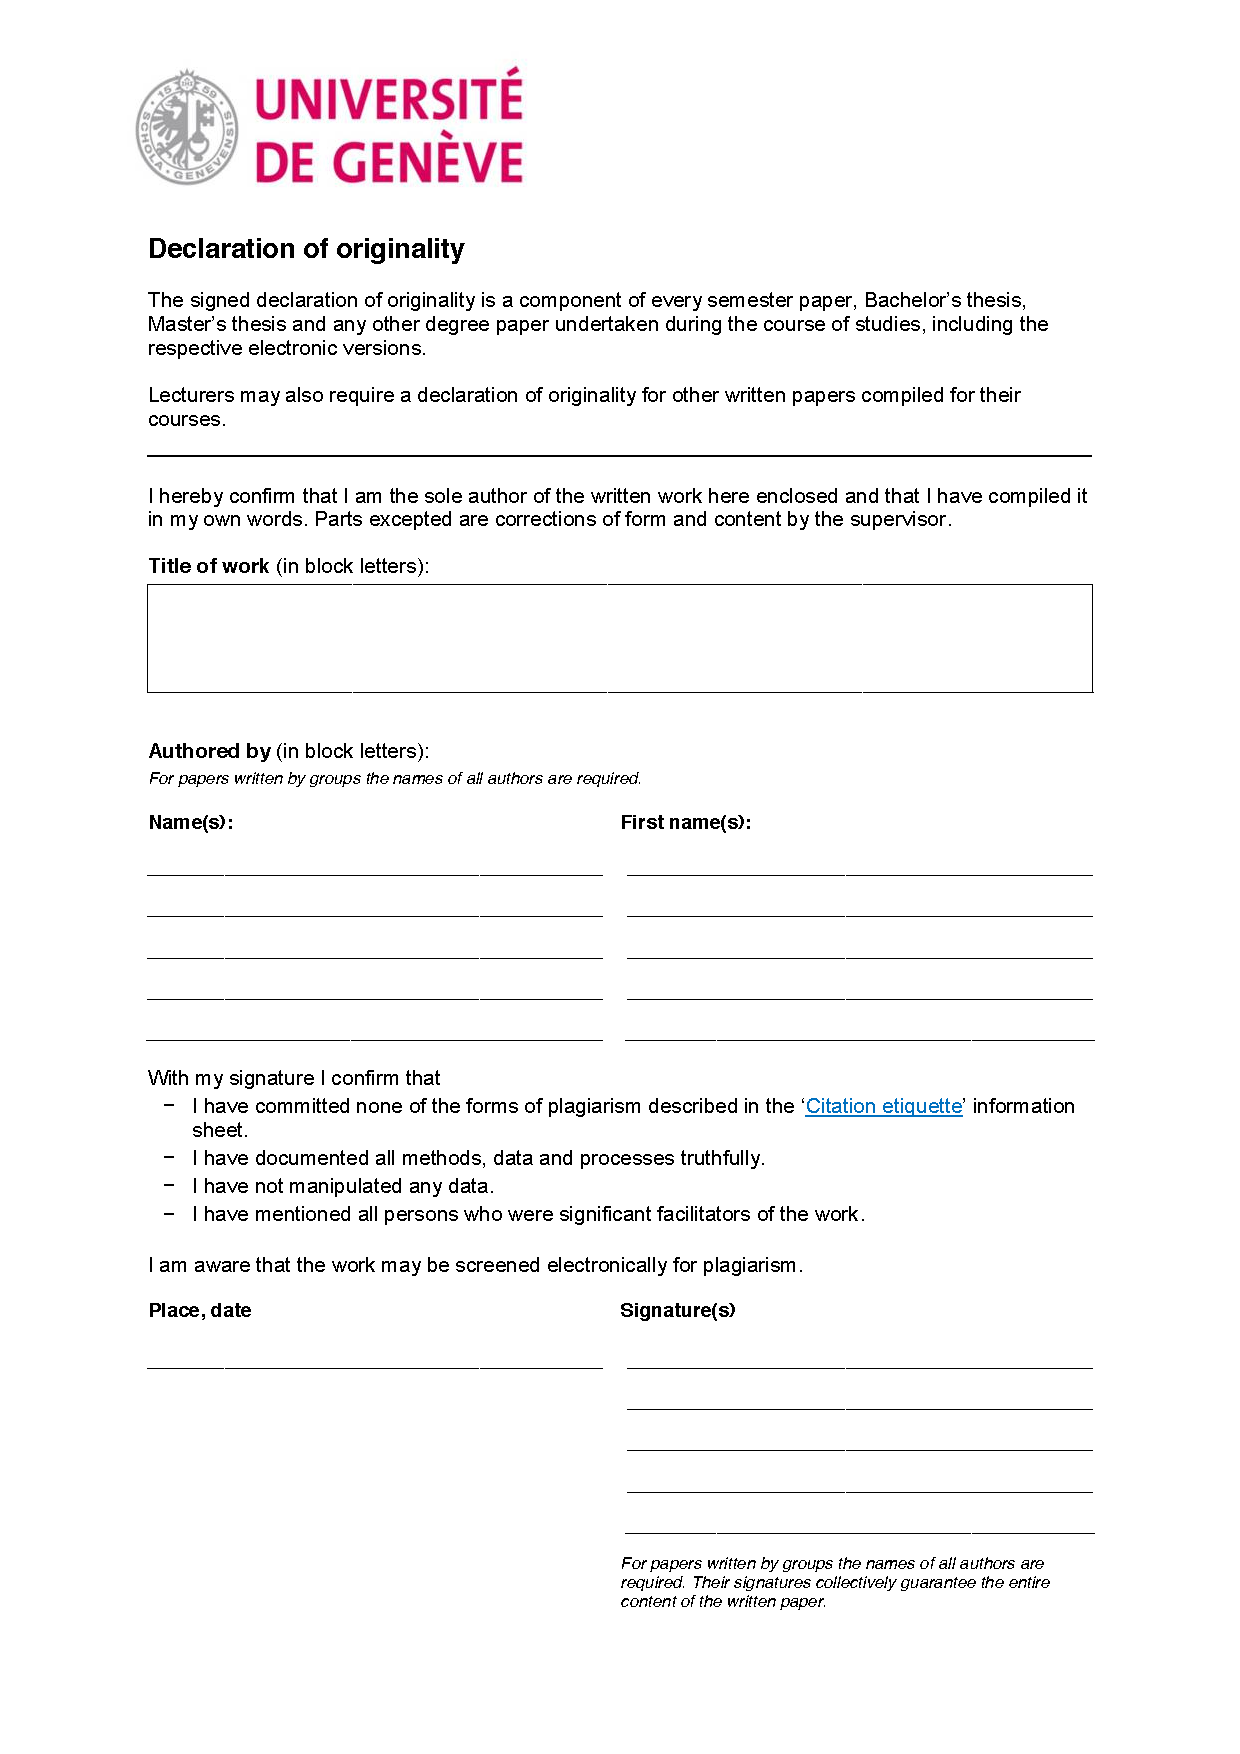
\includepdf[pages={-}]{declaration-originality.pdf}
\end{document}
